\documentclass[12pt,letterpaper,openany]{report} % openany evita páginas en blanco entre capítulos

% ===== Paquetes =====
\usepackage[spanish]{babel}
\usepackage[utf8]{inputenc}
\usepackage[T1]{fontenc}
\usepackage{setspace}
\usepackage{graphicx}
\usepackage{enumitem}
\usepackage{pifont}
\usepackage{times}
\usepackage{float}
\usepackage{array} 
\usepackage{longtable}
\usepackage{subcaption}
\usepackage{booktabs}
\usepackage{tocloft}
\usepackage[letterpaper,left=3cm,right=2.5cm,top=3cm,bottom=2.5cm]{geometry}
\usepackage{fancyhdr}
\usepackage{tabularx}
\usepackage{adjustbox}
\usepackage{ulem}

% Bibliografía (orden correcto)
\usepackage[natbibapa]{apacite} % <<< Formato APA
\usepackage{hyperref}           % <<< Siempre después de apacite

% ===== Encabezado con número arriba a la derecha =====
\pagestyle{fancy}
\fancyhf{}
\fancyhead[R]{\thepage}
\renewcommand{\headrulewidth}{0pt}

\fancypagestyle{plain}{%
  \fancyhf{}
  \fancyhead[R]{\thepage}
  \renewcommand{\headrulewidth}{0pt}
}

% === Estilo uniforme para títulos de capítulo ===
\usepackage{titlesec}
\titleformat{\chapter}[block]
  {\normalfont\bfseries\filcenter} % mismo estilo que resumen/abstract
  {} % sin número
  {0pt} % sin espacio extra antes del título
  {\normalsize} % tamaño igual a texto normal
\titlespacing*{\chapter}{0pt}{0pt}{1\baselineskip} % espacio antes y después

\doublespacing

\begin{document}
\let\origcleardoublepage\cleardoublepage
\let\cleardoublepage\relax

% ====== Portada y contraportada ======
\pagenumbering{gobble} % sin numeración
% Portada con marco y márgenes ajustados
\thispagestyle{empty} % sin número ni encabezado

\newgeometry{left=3cm,right=2.5cm,top=3cm,bottom=2.5cm}
\setlength{\fboxsep}{5pt} % padding interno del marco

\noindent\makebox[\linewidth]{%
\fbox{%
\begin{minipage}[t][\textheight][t]{\dimexpr\linewidth-2\fboxsep-2\fboxrule}%
\centering

\fontsize{12}{14}\selectfont
Universidad Central\\[0.3cm]
Facultad de Ingeniería y Ciencias Básicas\\[0.3cm]
Maestría en Analítica de Datos\\[1.2cm]

%[insertar imagen del logo de la universidad]

\includegraphics[width=6.5cm]{Imagenes/01_logo-ucentral.png}\\[1.5cm]

Predicción de variables meteorológicas usando una PINN basada en las ecuaciones de Navies-Stokes\\[1.2cm]

Tesis de Maestría\\[1.2cm]

S. Alejandro Gómez Ardila\\[1.2cm]
% Ricardo Luis Villegas Martínez\\[1.2cm]

Trabajo de grado como requisito para optar el título de:\\
Magister en analítica de datos\\[1.2cm]

Bogotá, Colombia\\
2026

\end{minipage}%
}%
}

\restoregeometry
\newpage % aquí cerramos la página nosotros

\clearpage
% Contraportada
\thispagestyle{empty} % sin número de página
\newgeometry{left=3cm,right=2.5cm,top=3cm,bottom=2.5cm}

\begin{center}
\fontsize{12}{14}\selectfont
Universidad Central\\[0.3cm]
Facultad de Ingeniería y Ciencias Básicas\\[0.3cm]
Maestría en Analítica de Datos\\[1.2cm]

% [insertar imagen del logo de la universidad]

\includegraphics[width=6.5cm]{Imagenes/01_logo-ucentral.png}\\[1.5cm]

\\[1.2cm]

Tesis de Maestría\\[1.2cm]

S. Alejandro Gómez Ardila\\[0.8cm]
% Ricardo Luis Villegas Martínez\\[0.8cm]
\\[1.2cm]

Director\\[0.5cm]
Dr. Diego Roldán\\[2cm]

Bogotá, Colombia\\
2026
\end{center}

\restoregeometry
\newpage

\clearpage

% ====== Aprobación y preliminares ======
\pagenumbering{arabic}
\setcounter{page}{3} % primera página numerada

\thispagestyle{empty} % sin número en esta página

\begin{center}
Aprobación
\end{center}

\vspace{1cm}

% ========== Director y Codirector ==========
\noindent
\begin{minipage}[t]{0.48\textwidth}
\raggedright
Director(a) de Tesis\\[1.0cm]
\rule{7cm}{0.4pt}\\
Firma\\
Nombres Completos\\
Títulos
\end{minipage}
\hfill
\begin{minipage}[t]{0.48\textwidth}
\raggedright
Codirector(a) de Tesis\\[1.0cm]
\rule{7cm}{0.4pt}\\
Firma\\
Nombres Completos\\
Títulos
\end{minipage}

\vspace{1.2cm}

% ========== Jurados ==========
\begin{center}
Jurados de la Tesis
\end{center}

\vspace{0.8cm}

\noindent
\begin{minipage}[t]{0.48\textwidth}
\raggedright
Jurado\\[1.0cm]
\rule{7cm}{0.4pt}\\
Firma\\
Nombres Completos\\
Títulos
\end{minipage}
\hfill
\begin{minipage}[t]{0.48\textwidth}
\raggedright
Jurado\\[1.0cm]
\rule{7cm}{0.4pt}\\
Firma\\
Nombres Completos\\
Títulos
\end{minipage}

\vspace{1.0cm}

\noindent
\begin{minipage}[t]{0.48\textwidth}
\raggedright
Jurado\\[1.0cm]
\rule{7cm}{0.4pt}\\
Firma\\
Nombres Completos\\
Títulos
\end{minipage}

% ========== Fecha de sustentación al fondo ==========
\vfill
\begin{center}
[Fecha de sustentación]
\end{center}

\clearpage
\begin{center}
\textbf{Dedicatoria}
\end{center}
% Contenido de la sección Dedicatoria

\begin{itemize}[label=\ding{51}] % 51 = ✔
    \item Se sugiere escribir en letra \textit{cursiva}
    \item El autor de este trabajo lo dedica en forma especial a personas o escribir citas célebres
\end{itemize}

\vspace{10pt}

\begin{flushright}
A mis padres
\end{flushright}

\begin{flushright}
\textit{'Hay q'} \\
\textit{Anónimo}
\end{flushright}


\clearpage
\begin{center}
\textbf{Agradecimientos}
\end{center}
% Contenido de la sección Agradecimientos

\begin{itemize}[label=\ding{51}] % 51 = ✔
    \item Esta sección es opcional.
    \item El autor agradece a las personas o instituciones que colaboraron en la realización del trabajo.
    \item Si se incluye esta sección, deben aparecer los nombres completos, los cargos y su aporte al trabajo.
\end{itemize}




\clearpage
% --------- Resumen ----------
\begin{flushleft} % Asegura alineación izquierda para todo
\begin{center}
\textbf{Resumen}
\end{center}
\vspace{0.8\baselineskip}

% Este resumen contiene:
% \begin{itemize}
%     \item Una introducción de la importancia del trabajo.
%     \item La descripción del problema y su alcance.
%     \item Los objetivos generales y específicos.
%     \item Los métodos.
%     \item Los resultados.
%     \item Las conclusiones de lo encontrado en el trabajo de investigación.
% \end{itemize}

% Se debe tener en cuenta:
% \begin{itemize}
%     \item Usar una extensión máxima de 500 palabras.
%     \item Que el resumen sea analítico, es decir, con información cuantitativa y cualitativa.
%     \item Al final del resumen se deben usar palabras claves tomadas del texto, las cuales permiten la % recuperación de la información.
% \end{itemize}

Este proyecto desarrolla y evalúa una Red Neuronal Físicamente Informada (Physics-Informed Neural Network, PINN) para predecir componentes del viento ($u_x$, $u_y$) y presión atmosférica ($p$) en el litoral Caribe colombiano durante diciembre de 2025. El dominio se construyó con datos horarios de estaciones meteorológicas de Datos Abiertos Colombia. El problema abordado consiste en estimar un campo continuo espacio-temporal a partir de observaciones puntuales, incorporando de manera explícita restricciones físicas de las ecuaciones de Navier-Stokes invíscidas en la función de pérdida.
\vspace{0.5em}

La metodología comprendió la carga y depuración de datos con exclusión de cuatro estaciones por criterios de calidad, proyección cartesiana y normalización adimensional, construcción de una malla de colocación para imponer las restricciones físicas en el dominio, entrenamiento de la arquitectura de red neuronal de 12 capas ocultas y 1200 neuronas por capa durante 2000 épocas, y un barrido sistemático de hiperparámetros de resolución de malla y peso físico de las ecuaciones, más una corrida final con la totalidad de los datos disponibles. Se evaluaron 13 experimentos en total.

Los resultados consolidados identifican como mejor configuración global la corrida con cobertura completa de datos (13.392 registros), con error observacional promedio $\bar{MSE}_{obs}=0{,}76$ y residual de Navier-Stokes $0{,}01$. En el subconjunto de 300 registros por estación, la mejor configuración alcanzó $\bar{MSE}_{obs}=0{,}85$. El estudio evidenció una tensión entre ajuste observacional y cumplimiento físico, y mostró que aumentar la cobertura temporal de datos mejora simultáneamente ambos criterios.

\vspace{1em}
\textbf{Palabras clave:} [Redes Neuronales Físicamente Informadas, PINN, Navier-Stokes, predicción meteorológica, Caribe colombiano, aprendizaje profundo]
\end{flushleft}

% mínimo 5 y máximo 7 palabras, use lenguaje técnico-científico



\clearpage
% --------- Abstract ----------
\begin{flushleft} % Asegura alineación izquierda para todo
\begin{center}
\textbf{Abstract}
\end{center}
\vspace{0.8\baselineskip}

This project develops and evaluates a Physics-Informed Neural Network (PINN) to predict wind components ($u_x$, $u_y$) and atmospheric pressure ($p$) over the Colombian Caribbean coast during December 2025. The study addresses the reconstruction of a continuous spatio-temporal field from sparse station observations while enforcing physical consistency through inviscid Navier-Stokes constraints.
\vspace{0.5em}

The workflow included data loading and cleaning (with four stations excluded for quality issues), Cartesian projection and dimensionless normalization, collocation mesh construction, and training of a 12-hidden-layer architecture with 1200 neurons per layer for 2000 epochs. A systematic hyperparameter sweep over mesh resolution and physics-loss weight was executed, followed by a final run using all available records. In total, 13 experiments were evaluated.

The best global configuration, trained with 13,392 records, achieved an average observational error of $\bar{MSE}_{obs}=0.76$ and a Navier-Stokes residual of $0.01$. Within the 300-records-per-station subset, the best configuration reached $\bar{MSE}_{obs}=0.85$. Results show a trade-off between observational fit and physical compliance, and indicate that increasing temporal data coverage simultaneously improves both criteria.

\vspace{1em}
\textbf{Keywords:} [Physics-Informed Neural Networks, PINN, Navier-Stokes, weather prediction, Colombian Caribbean, deep learning]
\end{flushleft}

\clearpage

% ====== Índice general ======
\clearpage
\tableofcontents
\clearpage

% ====== Lista de figuras ======
\clearpage
\listoffigures
\clearpage

% ====== Lista de tablas ======
\clearpage
\listoftables
\clearpage

% ====== Lista de siglas ======
\clearpage
% === Lista de siglas y abreviaturas ===
\chapter*{Lista de siglas y abreviaturas}
\addcontentsline{toc}{chapter}{Lista de siglas y abreviaturas} % opcional

\begin{table}[H]
\centering
\renewcommand{\arraystretch}{1.3} % más espacio entre filas
\setlength{\tabcolsep}{6pt}       % menos espacio horizontal entre columnas
\begin{tabularx}{\textwidth}{|c|X|X|}
\hline
\textbf{Sigla} & \textbf{Inglés} & \textbf{Español} \\ \hline
PINN   & Physics-Informed Neural Network & Red neuronal informada por la física \\ \hline
EDP    & Partial Differential Equation & Ecuación diferencial parcial \\ \hline
NWP    & Numerical Weather Prediction & Predicción numérica del tiempo \\ \hline
WRF    & Weather Research and Forecasting & Modelo de investigación y pronóstico del tiempo \\ \hline
RMSE   & Root Mean Square Error & Raíz del error cuadrático medio \\ \hline
MAE    & Mean Absolute Error & Error absoluto medio \\ \hline
LSTM   & Long Short-Term Memory & Memoria a largo y corto plazo \\ \hline
RNN    & Recurrent Neural Network & Red neuronal recurrente \\ \hline
CPU    & Central Processing Unit & Unidad central de procesamiento \\ \hline
GPU    & Graphics Processing Unit & Unidad de procesamiento gráfico \\ \hline
\end{tabularx}
\caption{Lista de siglas y abreviaturas utilizadas en el documento.}
\end{table}



\clearpage

% ====== Lista de anexos ======
\clearpage
% === Lista de siglas y abreviaturas ===
\chapter*{Lista de anexos}
\addcontentsline{toc}{chapter}{Lista de anexos}

\noindent Anexo 1. Encuesta \dotfill 45 \\
\noindent Anexo 2. Código fuente del modelo de clasificación \dotfill 50 \\
\\



\clearpage

% ====== Cuerpo del trabajo ======
\chapter*{Introducción} % sin número
\addcontentsline{toc}{chapter}{Introducción}

El estudio del clima ha sido una preocupación constante a lo largo de la historia de la humanidad. Desde las antiguas civilizaciones, que basaban sus predicciones en la observación empírica de fenómenos naturales —como la formación de nubes, los patrones de viento o los cambios de temperatura \citep{ossendrijver2021babylonian}—, hasta los científicos contemporáneos que emplean sofisticados modelos físico-matemáticos para describir el comportamiento atmosférico \citep{lorenz1963deterministic}, la necesidad de anticipar las condiciones climáticas ha persistido como un desafío fundamental.

En la actualidad, la capacidad de predecir variables meteorológicas con precisión es vital para la planificación urbana, la agricultura, la gestión de recursos hídricos, la aviación, la generación de energía eólica y la prevención de desastres naturales, como tormentas o inundaciones \citep{wmo2023state}. No obstante, la atmósfera es un sistema caótico gobernado por ecuaciones no lineales, lo que ocasiona que pequeñas variaciones en las condiciones iniciales generen divergencias significativas en las predicciones; este fenómeno es conocido como el “efecto mariposa” \citep{lorenz1972predictability}. Esta complejidad inherente convierte la reconstrucción y proyección de estados climáticos en una tarea computacional y teóricamente exigente.

Con el desarrollo de sistemas de computación de alto rendimiento, la recolección de datos meteorológicos ha experimentado una revolución. Estaciones terrestres, boyas oceánicas, radares Doppler y satélites de observación —como los programas ERA5 del ECMWF o GOES de la NASA/NOAA \citep{aragao2022cyclonic}— proporcionan flujos masivos de información en tiempo real, capturando variables como temperatura, presión atmosférica, velocidad y dirección del viento, humedad y radiación solar \citep{hasler1989automatic}.

Sin embargo, los métodos tradicionales para procesar estos datos, basados en simulaciones numéricas como los Modelos de Circulación General (GCMs) \citep{guilyardi2009coupled} o el Weather Research and Forecasting Model (WRF) \citep{skamarock2001wrf}, enfrentan dos limitaciones principales:
\begin{enumerate}
    \item Alto costo computacional: La necesidad de resolver ecuaciones diferenciales complejas, como las de Navier-Stokes, en una malla tridimensional con alta resolución espacial y temporal.

    \item Dependencia de parametrizaciones empíricas: Muchos procesos físicos, como la formación de nubes o la turbulencia, ocurren a escalas menores que la resolución de la malla del modelo. Esto obliga a realizar aproximaciones mediante parametrizaciones basadas en relaciones simplificadas, lo que introduce incertidumbre en los resultados.
\end{enumerate}

En este escenario destaca el potencial de las Redes Neuronales Físicamente Informadas (PINNs), una rama de la inteligencia artificial que busca cerrar la brecha entre los modelos basados exclusivamente en datos y las leyes físicas fundamentales. Las PINNs son arquitecturas que incorporan ecuaciones diferenciales parciales (EDPs), como las de Navier-Stokes para fluidos o la de conservación de la energía, directamente en su función de pérdida durante el entrenamiento \citep{cai2021physics}.

A diferencia de las redes neuronales tradicionales, las PINNs no solo aprenden correlaciones estadísticas, sino que garantizan la consistencia con las leyes físicas. Esto permite realizar entrenamientos sin necesidad de volúmenes masivos de datos, ya que el conocimiento físico actúa como un regularizador. Además, resultan sumamente eficaces para resolver problemas inversos, permitiendo inferir parámetros ocultos a partir de observaciones dispersas.

Aunque se ha probado su eficacia en la predicción de flujos turbulentos y la asimilación de datos heterogéneos, su aplicación a escalas locales para la reconstrucción de campos de viento y presión a partir de estaciones meteorológicas dispersas sigue siendo un área poco explorada. Moreno Soto et al. \cite{morenosoto2024pinns} presentaron una de las primeras aplicaciones de PINNs a la reconstrucción meteorológica de alta resolución a partir de estaciones dispersas, sirviendo como referencia metodológica para este trabajo. En este proyecto, el caso de estudio corresponde a la región Caribe de Colombia, a partir de registros de estaciones del IDEAM disponibles en el portal de Datos Abiertos Colombia. Los datos cubren el mes de diciembre de 2025 e incluyen posición geográfica, tiempo, velocidad y dirección del viento, presión y temperatura. A partir de estas observaciones, se plantea una PINN que recibe como entrada dos coordenadas espaciales y una variable temporal $(x, y, t)$, y predice la presión y las componentes cartesianas del viento $(vel_x, vel_y)$ sobre una malla espacio-temporal, con el fin de estimar condiciones atmosféricas en puntos no instrumentados.
\clearpage
\chapter*{Planteamiento}

Las estaciones meteorológicas ofrecen mediciones confiables de variables atmosféricas, pero su distribución espacial suele ser irregular y limitada a puntos discretos del territorio. En consecuencia, cuando se requiere analizar el comportamiento del viento y la presión sobre una región completa, aparecen vacíos de información en zonas donde no existe instrumentación. Esta limitación es especialmente relevante cuando se pretende construir mapas continuos de condiciones atmosféricas o realizar predicciones locales con resolución espacio-temporal fina.

En el caso de estudio considerado en este proyecto, se dispone de registros de estaciones meteorológicas ubicadas en la región Caribe de Colombia, obtenidos del portal de Datos Abiertos Colombia (\url{https://www.datos.gov.co/}). Los datos corresponden al mes de diciembre de 2025 y provienen de estaciones del IDEAM distribuidas en los departamentos de Atlántico, Bolívar, Magdalena, Sucre y Córdoba. Cada registro contiene coordenadas geográficas, tiempo, velocidad del viento, dirección del viento, presión y temperatura. Sin embargo, estos datos no describen por sí solos el estado atmosférico continuo del dominio, ya que solo representan observaciones puntuales y no una malla completa del fenómeno.

De esta situación surge la siguiente pregunta de investigación:

\begin{quote}
¿Cómo construir un modelo basado en PINNs que, a partir de registros meteorológicos dispersos y de las ecuaciones de Navier-Stokes, permita estimar la presión y las componentes del viento sobre una malla espacio-temporal en puntos donde no existen estaciones de medición?
\end{quote}

\textbf{Justificación}

La región Caribe colombiana presenta una marcada variabilidad climática impulsada por la migración de la Zona de Convergencia Intertropical (ZCIT) y la actividad de la corriente de bajo nivel del Caribe (\textit{Caribbean Low-Level Jet}, CLLJ), localizada entre los 13° y 15°\,N con núcleo por debajo de los 900\,hPa, que registra velocidades máximas del orden de 12\,m/s durante la época seca (diciembre--marzo) y el verano boreal (junio--agosto) \citep{perez2018seabreeze}. Precisamente durante la época seca, los vientos alisios del noreste alcanzan su mayor intensidad sobre la franja costera \citep{ideam2005atlas}, lo que confiere especial relevancia climática al periodo de diciembre de 2025 considerado en este trabajo. Adicionalmente, las fases del ENOS modulan el régimen regional: durante El Niño se registra déficit de precipitación en el Caribe colombiano, en tanto que La Niña induce la respuesta contraria \citep{pabon2017fenomenos}. No obstante esta relevancia, la red de monitoreo del IDEAM en los cinco departamentos del área de estudio (Atlántico, Bolívar, Magdalena, Sucre y Córdoba) cuenta únicamente con 18 estaciones válidas distribuidas sobre un dominio de 404,7\,km (norte--sur) por 252,2\,km (este--oeste), lo que equivale a una densidad aproximada de 1,8 estaciones por cada 10.000\,km², insuficiente para caracterizar la variabilidad espacial continua del campo de viento y presión, como se ilustra en la Figura~\ref{fig:mapa_estaciones}.

La relevancia del problema radica en que una estimación continua del campo de viento y presión mejora la interpretación de fenómenos atmosféricos locales y sirve como soporte para tareas de monitoreo, planeación urbana y análisis ambiental. Desde el punto de vista computacional, una PINN ofrece la ventaja de combinar observaciones reales con conocimiento físico, evitando depender exclusivamente de interpolaciones estadísticas o de simulaciones numéricas de alto costo.

Adicionalmente, la descomposición de la velocidad y la dirección del viento en componentes cartesianas permite representar el flujo de forma más adecuada para el aprendizaje del modelo, mientras que la incorporación explícita del tiempo hace posible estudiar la evolución del sistema sobre una malla espacio-temporal. Por ello, el proyecto se justifica como un aporte metodológico para reconstruir condiciones atmosféricas locales con coherencia física en zonas parcialmente observadas.



\clearpage
\chapter{Objetivos}
% Contenido de la sección Objetivos

\textbf{Objetivo General}

Desarrollar un modelo de Redes Neuronales Físicamente Informadas (PINNs) basado en las ecuaciones de Navier-Stokes y en registros de estaciones meteorológicas del litoral Caribe colombiano, con el fin de estimar sobre una malla espacio-temporal la presión atmosférica y las componentes del viento en puntos donde no existen mediciones directas.

\vspace{25pt}

\textbf{Objetivos Específicos}

\begin{enumerate}
    \item Organizar y preprocesar los registros de las estaciones meteorológicas del litoral Caribe colombiano, incluyendo coordenadas geográficas, series de tiempo, velocidad y dirección del viento, presión atmosférica y temperatura, para construir un conjunto de entrenamiento coherente y representativo del dominio espacio-temporal de estudio.

    \item Diseñar y entrenar una Red Neuronal Físicamente Informada (PINN) que incorpore las restricciones de las ecuaciones de Navier-Stokes en su función de pérdida, con el fin de estimar las componentes del viento y la presión atmosférica sobre una malla espacio-temporal que incluya ubicaciones sin medición directa.

    \item Evaluar cuantitativamente el desempeño del modelo mediante métricas de error estándar calculadas sobre datos de prueba retenidos, con el fin de determinar la capacidad de generalización espacial y temporal de la red entrenada.

\end{enumerate}



\clearpage
\chapter{Antecedentes}
% Contenido de la sección Antecedentes

\section{Modelos numéricos basados en ecuaciones diferenciales parciales.}

El núcleo de los Modelos de Predicción Numérica del Tiempo (NWP, por sus siglas en inglés) reside en sistemas de ecuaciones diferenciales parciales (EDP) no lineales, como las ecuaciones de Navier-Stokes. Estas gobiernan la dinámica de los fluidos atmosféricos mediante el acoplamiento con ecuaciones de conservación de masa, energía y humedad. Si bien las EDP capturan la física fundamental de la atmósfera, su resolución exacta enfrenta dos obstáculos críticos: la no linealidad intrínseca (por ejemplo, el término convectivo $\mathbf{u} \cdot \nabla \mathbf{u}$) y la sensibilidad caótica a las condiciones iniciales. En este último caso, errores mínimos ($\approx 0.1\%$ en las mediciones de presión) crecen exponencialmente, lo que limita la ventana de predicción a un máximo de $\approx 10$ días \citep{lorenz1963deterministic}.

Además, la discretización espaciotemporal mediante métodos de elementos o volúmenes finitos exige mallas con una resolución extremadamente alta (llegando a micras en las capas límite), lo que conlleva costos computacionales prohibitivos. Por ejemplo, el modelo del European Centre for Medium-Range Weather Forecasts (ECMWF) opera a resoluciones de $\approx 9$ km, consumiendo 2.5 millones de horas de CPU diarias \citep{ecmwf2023}. Para mitigar estos desafíos, han surgido alternativas eficientes como los esquemas Lagrange-Galerkin (LG). Estos enfoques discretizan la derivada material a lo largo de las trayectorias del flujo, transformando el problema no lineal en un sistema lineal de Stokes en cada paso de tiempo. Esto permite reducir los costos computacionales hasta en un $40\%$ en comparación con los métodos implícitos convencionales \citep{bermejo2016lagrange}.

Sin embargo, su implementación en mallas no estructuradas —fundamentales para los modelos atmosféricos regionales— requiere algoritmos especializados para calcular integrales de alto orden y localizar puntos en elementos de la malla. Estos procesos pueden consumir hasta el $60\%$ del tiempo de simulación \citep{bermejo2016lagrange}. Adicionalmente, los fenómenos de subescala (como la turbulencia y la convección) se modelan mediante parametrizaciones empíricas. Por ejemplo, el modelo WRF utiliza esquemas de convección como el de Kain-Fritsch para aproximar movimientos verticales en escalas inferiores a la resolución de la malla, lo que introduce una incertidumbre sistémica de $\approx 15\%$ en los pronósticos de precipitación \citep{skamarock2019wrf}.

Aunque estos métodos preservan las leyes físicas fundamentales, su escalabilidad está limitada por la necesidad de condiciones iniciales altamente precisas y recursos computacionales masivos, lo que motiva la continua búsqueda de enfoques alternativos.

\section{Métodos Estadísticos Clásicos.}
\subsection{Enfoques Clásicos: ARIMA y Procesos Gaussianos}

Como alternativa a los modelos de Predicción Numérica del Tiempo (NWP), diversas técnicas estadísticas, tales como ARIMA (AutoRegressive Integrated Moving Average) y los Procesos Gaussianos (GP), analizan patrones históricos para extrapolar tendencias meteorológicas. Entre sus principales ventajas se destacan:

\begin{itemize}
    \item ARIMA: Es altamente eficaz en pronósticos de corto plazo (menores a 72 horas), ya que logra capturar la estacionalidad mediante componentes autorregresivos y de diferenciación. Por ejemplo, en la predicción de brisas costeras, este modelo reduce el error cuadrático medio (RMSE) a $1.2 m/s$, frente a los $1.8 m/s$ de los modelos físicos simples \citep{montero2021arima}.
    
    \item Procesos Gaussianos: Permiten un modelado probabilístico de la incertidumbre en escalas subestacionales, lo cual es fundamental para la gestión de energías renovables. En parques eólicos del Mar del Norte, estos procesos predicen rachas de viento con intervalos de confianza del 95\% \citep{hojstrup2020gaussian}.
\end{itemize}

No obstante, la desconexión de estos métodos respecto a las leyes físicas los hace vulnerables ante eventos extremos sin precedentes, como las tormentas árticas en latitudes medias, fenómeno cuya frecuencia ha aumentado debido al cambio climático \citep{ipcc2023synthesis}. Esta limitación contrasta con el desempeño de los esquemas LG, los cuales garantizan la conservación de masa y energía mediante proyecciones de Galerkin; gracias a esta base física, logran un RMSE un 30\% menor en simulaciones de ciclones tropicales en comparación con los métodos puramente estadísticos \citep{bermejo2016lagrange}.

\subsection{Aprendizaje Automático Convencional}

Avances recientes han posicionado a modelos como GraphCast \citep{lam2023graphcast} y FourCastNet \citep{pathak2022fourcastnet} como competidores directos de los sistemas de Predicción Numérica del Tiempo (NWP, por sus siglas en inglés). Al ser entrenados con décadas de datos de reanálisis (como el conjunto ERA5), estos modelos omiten la integración paso a paso de Ecuaciones Diferenciales Parciales (EDP), lo que reduce los tiempos de computación de horas a escasos minutos. Un caso notable es FourCastNet, capaz de predecir trayectorias de huracanes con tres días de antelación y un margen de error de $\sim 50$ km, un rendimiento equiparable al modelo IFS del ECMWF \citep{pathak2022fourcastnet}.

No obstante, su naturaleza de 'caja negra' introduce desafíos críticos: se han observado inconsistencias físicas, tales como perfiles de presión no hidrostáticos o violaciones en la conservación de la energía de aproximadamente un $5\%$ en las capas altas de la atmósfera \citep{pathak2022fourcastnet}. Asimismo, su dependencia masiva de registros históricos ($\sim 5$ PB para un entrenamiento global) restringe su validez en escenarios climáticos sin precedentes, como el umbral de calentamiento global de $+2^\circ$C.

\subsection{Paradigmas Híbridos}

Para cerrar esta brecha, se han desarrollado enfoques híbridos que combinan la celeridad del aprendizaje automático (machine learning o ML) con el rigor físico de las ecuaciones en derivadas parciales (EDP). Un ejemplo destacado son los métodos Lagrange-Galerkin (LG) estabilizados, los cuales incorporan términos de proyección local para gestionar números de Reynolds elevados \citep{bermejo2016lagrange}. En simulaciones de flujos sobre turbinas eólicas, estos esquemas reducen las oscilaciones espurias en un 40 \% en comparación con los métodos no estabilizados. Paralelamente, las redes neuronales físicamente informadas (PINN) codifican las ecuaciones de Navier-Stokes directamente en sus funciones de pérdida; este enfoque logra un 30 \% más de precisión que los modelos de predicción numérica del tiempo (NWP) en pronósticos de intensificación rápida de huracanes \citep{yang2023physics}.
\clearpage
\chapter{Metodologia}

La metodología propuesta se organiza en cuatro etapas principales: adquisición y preparación de datos, formulación y entrenamiento de la PINN, diseño experimental de hiperparámetros, y evaluación del modelo entrenado. El propósito central es combinar observaciones dispersas de estaciones meteorológicas con restricciones físicas derivadas de las ecuaciones de Navier-Stokes para estimar variables atmosféricas en puntos no medidos sobre la región Caribe de Colombia.

\section{Datos de entrada}

Los datos provienen del portal de Datos Abiertos Colombia (\url{https://www.datos.gov.co/}), que publica registros históricos del IDEAM. Se utilizó el conjunto de registros de estaciones meteorológicas de la región Caribe correspondientes al mes de diciembre de 2025, cubriendo los departamentos de Atlántico, Bolívar, Magdalena, Sucre y Córdoba. El archivo consolidado contiene 16.368 registros horarios distribuidos en aproximadamente 22 estaciones.

La extensión geográfica del dominio de estudio fue calculada a partir de las coordenadas de las 18 estaciones que integran el conjunto de entrenamiento, una vez aplicados los criterios de exclusión descritos en la sección de preprocesamiento. La latitud varía entre $7{,}4750^{\circ}$\,N y $11{,}1150^{\circ}$\,N, y la longitud entre $76{,}2240^{\circ}$\,O y $73{,}9260^{\circ}$\,O. Aplicando la fórmula de Haversine, la extensión norte–sur es de aproximadamente 404{,}7\,km y la extensión este–oeste de 252{,}2\,km, con una diagonal total del dominio de 476{,}9\,km. La Tabla~\ref{tab:dominio_geografico} resume estas dimensiones.

\begin{table}[H]
\centering
\caption{Extensión geográfica del dominio de estudio}
\label{tab:dominio_geografico}
\begin{tabular}{ll}
\hline
Dimensión & Valor \\
\hline
Latitud mínima & $7{,}4750^{\circ}$ N \\
Latitud máxima & $11{,}1150^{\circ}$ N \\
Longitud mínima & $76{,}2240^{\circ}$ O \\
Longitud máxima & $73{,}9260^{\circ}$ O \\
Extensión N--S & 404{,}7 km \\
Extensión E--O & 252{,}2 km \\
Diagonal del dominio & 476{,}9 km \\
Resolución de malla (barrido) & $R = 0{,}1^{\circ}$ ($\approx$ 11{,}1 km) \\
Latitud media del centroide & $9{,}295^{\circ}$ N \\
\hline
\end{tabular}
\end{table}

Las estaciones se concentran en la franja costera de los cinco departamentos analizados; la extensión este–oeste (252{,}2\,km) es notablemente menor que la extensión norte–sur (404{,}7\,km), lo que refleja la distribución lineal de la red de observación a lo largo del litoral. Las zonas del interior continental y la franja marítima carecen de cobertura directa, lo que refuerza la motivación del enfoque propuesto.

Cada observación incluye las siguientes variables:

\begin{itemize}
	\item Identificador y posición geográfica de la estación (latitud, longitud, altitud).
	\item Marca temporal expresada en segundos desde el inicio del periodo.
	\item Velocidad del viento (m/s) y dirección del viento (grados).
	\item Presión atmosférica (mbar).
	\item Temperatura del aire (°C).
\end{itemize}

\subsection{Caracterizacion descriptiva inicial del conjunto}

Como apoyo a la descripcion de los datos de entrada, la Figura~\ref{fig:serie_temporal_datos_caribe} resume el comportamiento temporal de las variables registradas durante el periodo de estudio. Esta evidencia visual permite identificar variabilidad intraperiodo y cambios de escala entre variables, aspectos que motivan las etapas de preprocesamiento y escalamiento descritas en las subsecciones siguientes.

% IMAGEN PENDIENTE: docs/descripcion_datos/em_caribe_time_series.png
% \begin{figure}[H]
% \centering
% 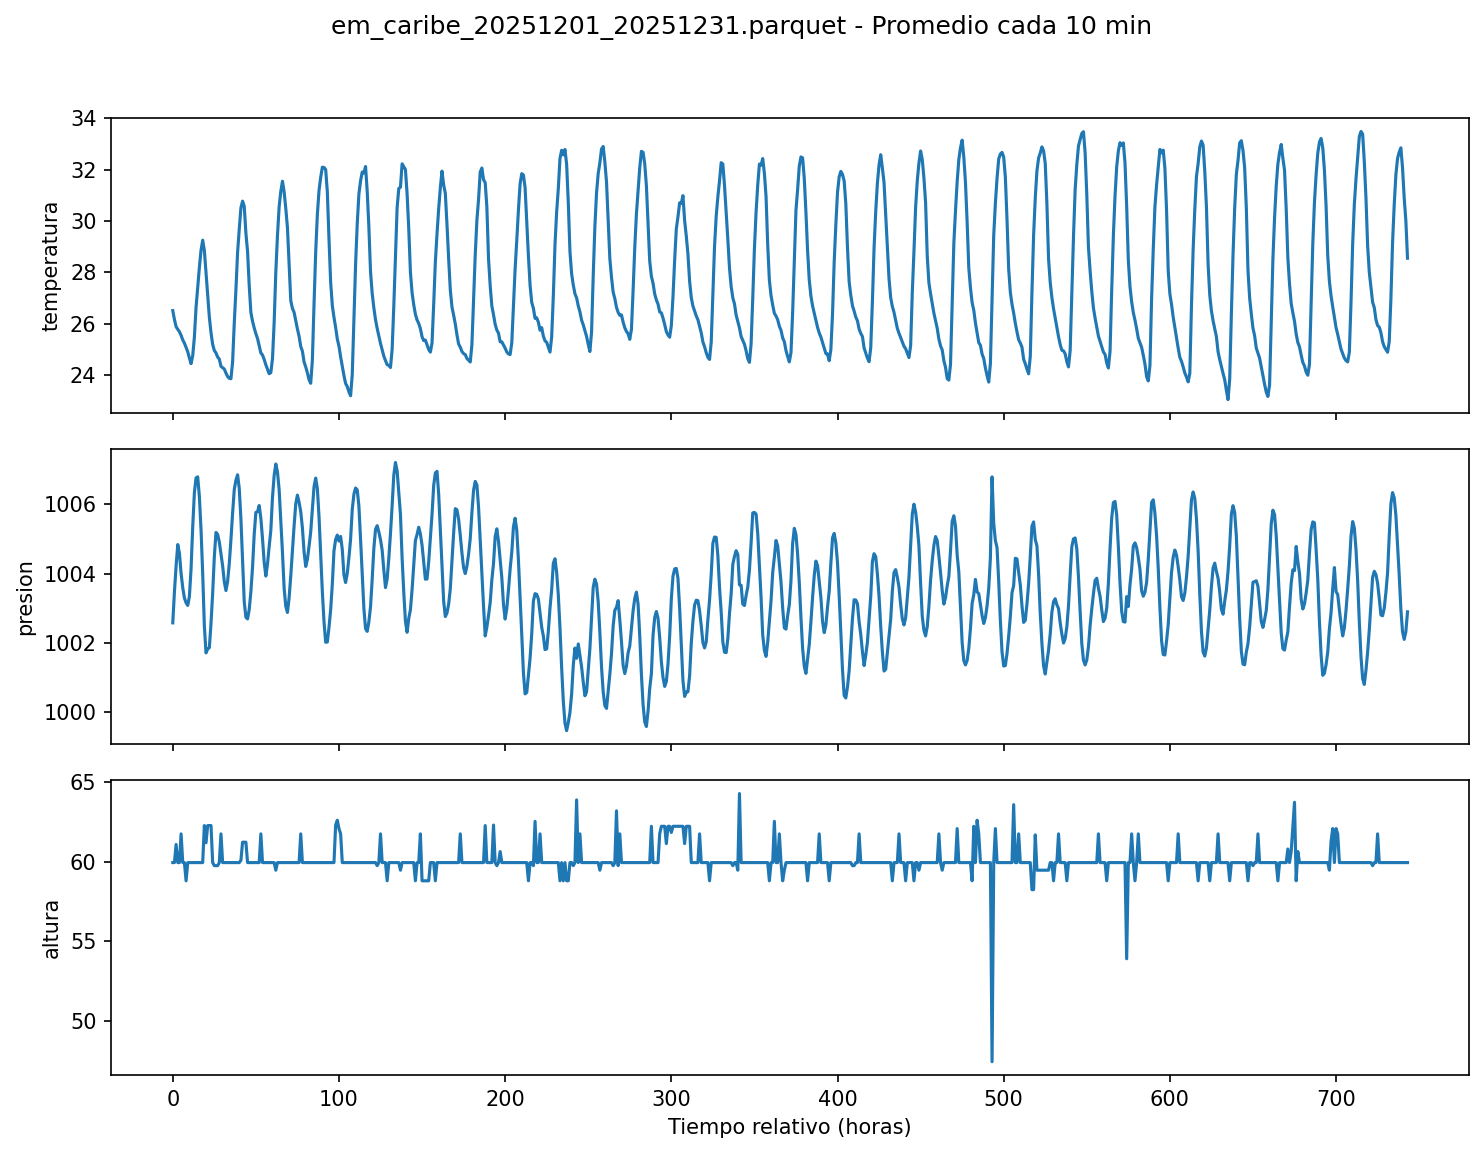
\includegraphics[width=0.95\textwidth]{docs/descripcion_datos/em_caribe_time_series.png}
% \caption{Serie temporal descriptiva de variables meteorologicas del conjunto Caribe para diciembre de 2025. La figura se incorpora como evidencia exploratoria del comportamiento temporal previo al entrenamiento de la PINN.}
% \label{fig:serie_temporal_datos_caribe}
% \end{figure}

\section{Preprocesamiento de la información}

El pipeline de preprocesamiento ejecuta las siguientes etapas en secuencia:

\subsection{Selección y exclusión de estaciones}

Se excluyen cuatro estaciones que presentan anomalías críticas en presión o en las componentes de viento. La Tabla~\ref{tab:estaciones_excluidas} detalla los criterios de exclusión aplicados. Tras la exclusión, se retienen 18 estaciones válidas, distribuidas geográficamente a lo largo de los cinco departamentos del área de estudio, como se ilustra en la Figura~\ref{fig:mapa_estaciones}.

\begin{table}[H]
\centering
\caption{Estaciones excluidas y criterio de exclusión aplicado}
\label{tab:estaciones_excluidas}
\begin{tabular}{lll}
\hline
Código de estación & Anomalía detectada        & Variable afectada \\\\
\hline
0025025380         & Presión anómalamente alta & $p$               \\\\
0025025030         & Error elevado             & $u_x$             \\\\
0025025190         & Error elevado             & $u_x$             \\\\
0015015100         & Error elevado             & $u_x$             \\\\
\hline
\end{tabular}
\end{table}

En el barrido de hiperparámetros se seleccionan los primeros 300 registros por estación, ordenados cronológicamente, lo que produce un subconjunto rectangular de $18 \times 300 = 5\,400$ registros. Una corrida adicional posterior utilizó la totalidad de los registros disponibles ($18 \times 744 = 13\,392$ registros) con la configuración óptima.

\begin{figure}[H]
\centering
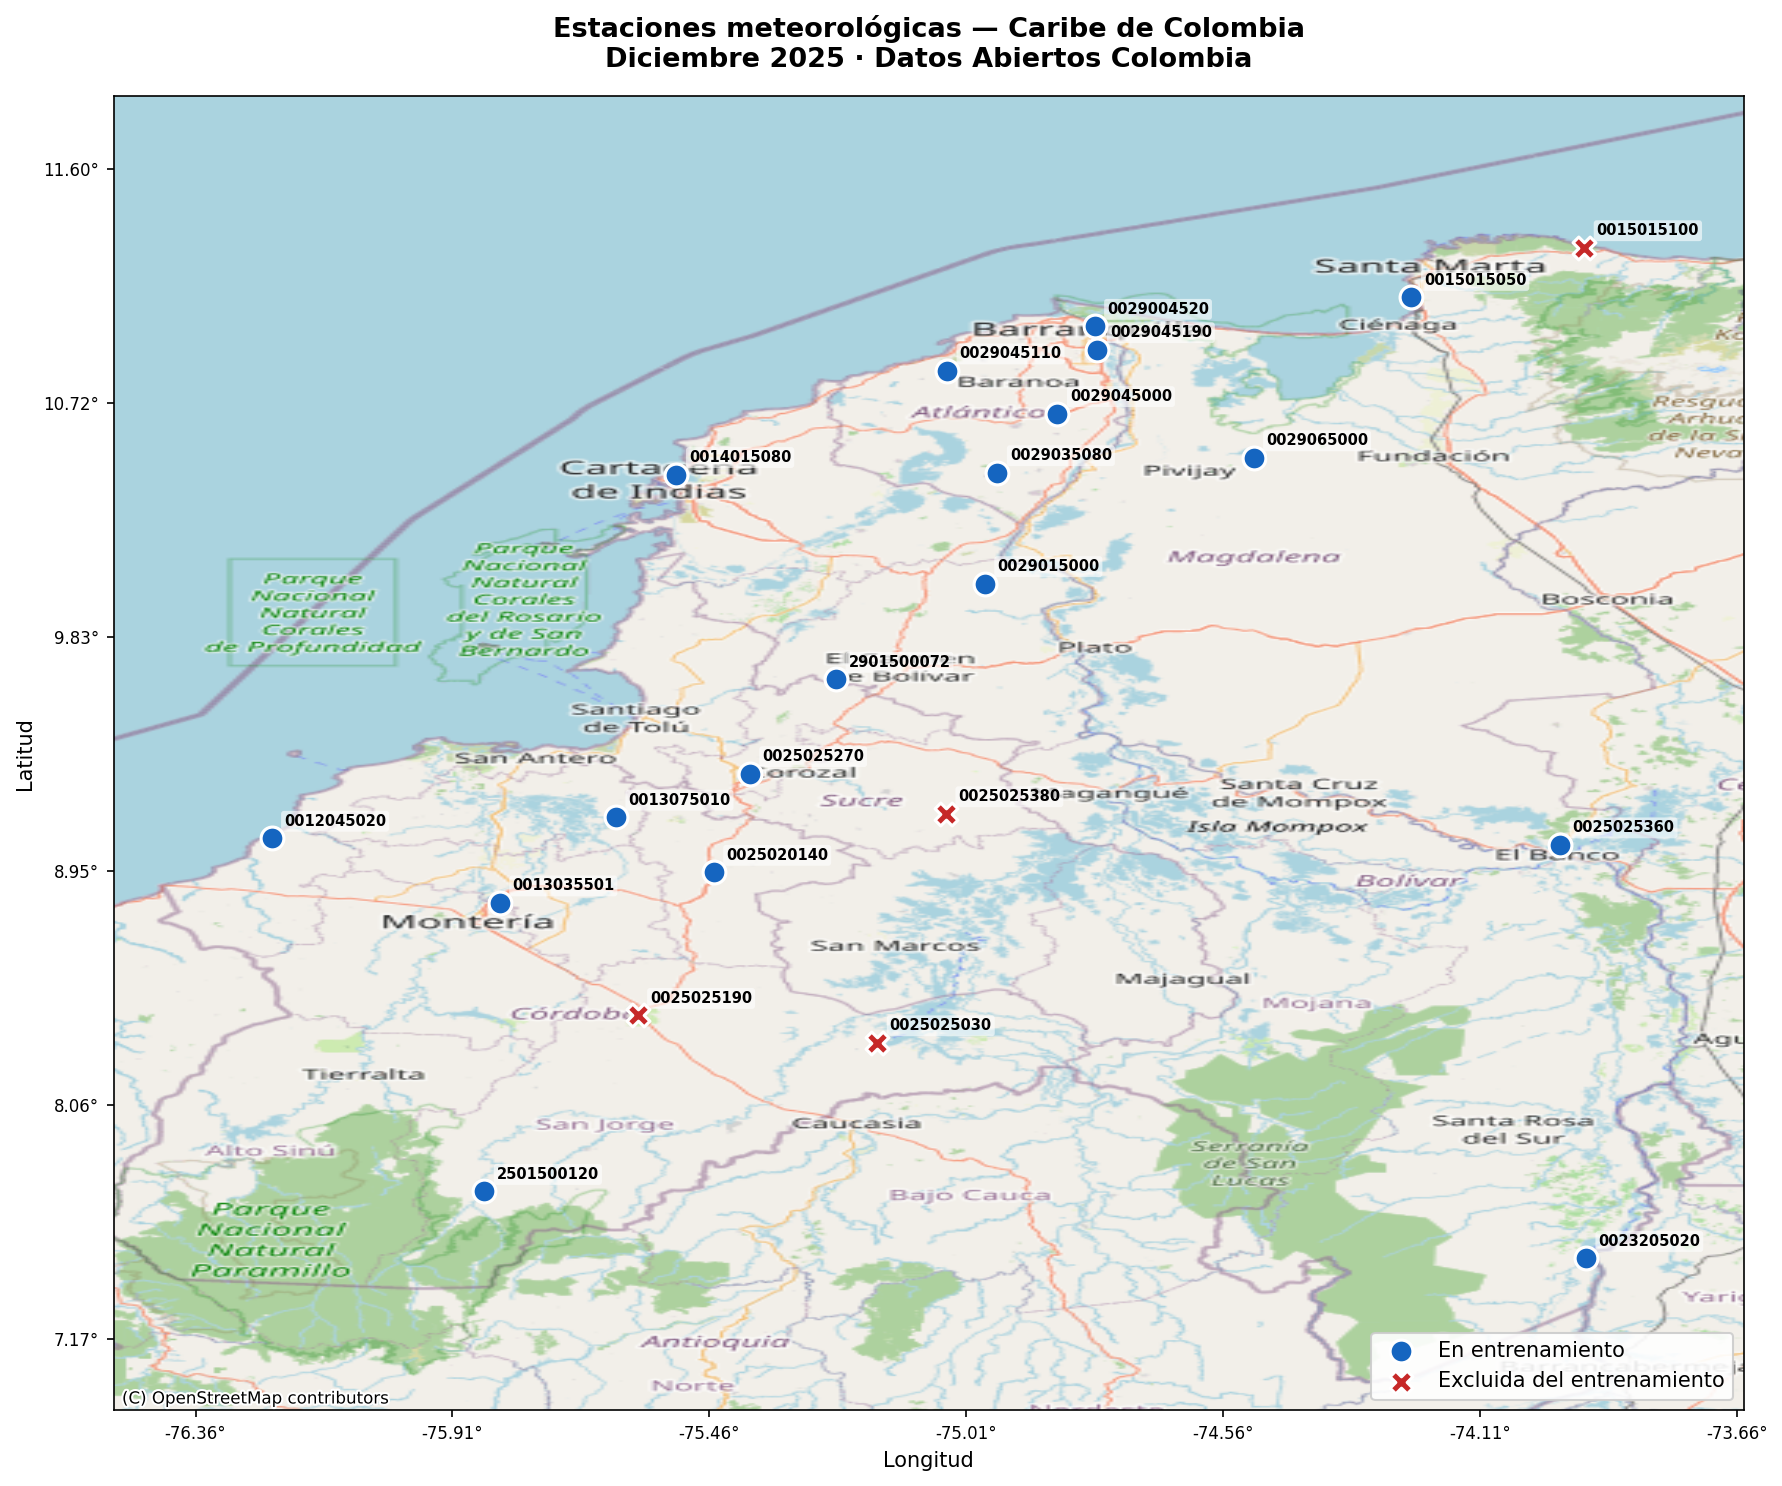
\includegraphics[width=0.85\textwidth]{Imagenes/mapa_estaciones_caribe.png}
\caption{Distribución geográfica de las estaciones meteorológicas del IDEAM en la región Caribe de Colombia. Los marcadores azules corresponden a las 18 estaciones válidas incluidas en el entrenamiento; los marcadores rojos identifican las 4 estaciones excluidas por anomalías en presión o en las componentes de viento.}
\label{fig:mapa_estaciones}
\end{figure}

\subsection{Descomposición del viento y proyección cartesiana}

La velocidad y la dirección del viento se descomponen en componentes cartesianas $u_x$ (componente Este–Oeste) y $u_y$ (componente Norte–Sur). Las coordenadas geográficas (latitud $\varphi$, longitud $\lambda$) se convierten a distancias en metros mediante aproximación de arco de círculo con radio terrestre $R_T = 6\,378\,000\,\text{m}$. Sea $(x_c, y_c)$ el centroide geográfico del dominio; entonces:

\[
x_i = R_T \cdot \sin\left(\frac{\pi}{180}\,\Delta\lambda_i\right), \qquad y_i = R_T \cdot \sin\left(\frac{\pi}{180}\,\Delta\varphi_i\right)
\]

donde $\Delta\lambda_i$ y $\Delta\varphi_i$ son los desplazamientos angulares respecto al centroide. Esta transformación produce un dominio cartesiano localizado en la región Caribe, con origen en el centroide. Las unidades resultantes son metros.

\subsection{Corrección de presión al nivel del mar}

La presión medida en cada estación se corrige al nivel del mar usando el modelo de atmósfera estándar internacional (ISA):

\[
P_{\text{corr}} = P \cdot \left(1 - \frac{0{,}0065 \cdot Z}{T + 273{,}15 + 0{,}0065 \cdot Z}\right)^{-5{,}257}
\]

donde $Z$ es la altitud de la estación en metros y $T$ es la temperatura en °C.

\subsection{Adimensionalización}

Todas las variables se adimensionalizan antes del entrenamiento para que la red opere con magnitudes comparables. Las escalas de referencia se calculan a partir de los propios datos:

\begin{itemize}
	\item $L$: rango máximo entre desplazamientos en $x$ o $y$ (escala de longitud).
	\item $W$: escala de velocidad observada, calculada a partir de los datos de viento.
	\item $\rho W^2$: presión dinámica de referencia (escala de presión).
	\item $T$: horizonte temporal total del período de estudio ($T = N_{\text{DIAS}} \cdot 86\,400\,\text{s}$).
\end{itemize}

Las transformaciones aplicadas son:

\[
x_{\text{norm}} = \frac{x}{L}, \quad y_{\text{norm}} = \frac{y}{L}, \quad t_{\text{norm}} = \frac{t}{T}
\]
\[
u_{\text{norm}} = \frac{u_x}{W}, \quad v_{\text{norm}} = \frac{u_y}{W}, \quad p_{\text{norm}} = \frac{p}{\rho W^2}
\]

El reescalado de presión por su desviación estándar ($\sigma_p = 1{,}9656$) representa una corrección adicional para equilibrar el rango de la presión normalizada con el de las velocidades, reduciendo asimetría numérica en la función de pérdida combinada.

\section{Definición de entradas y salidas del modelo}

La PINN recibe tres variables de entrada:
\[
(x, y, t)
\]
donde $x$ e $y$ representan la posición espacial normalizada y $t$ el tiempo normalizado. A partir de estas entradas, la red produce tres salidas:
\[
(vel_u,\ vel_v,\ p)
\]
correspondientes a las componentes cartesianas del viento y la presión, todas en escala adimensional.

\section{Arquitectura de la red}

La red neuronal implementa la capa \texttt{GammaBiasLayer}, una extensión de la capa lineal estándar que incorpora \textit{Weight Normalization} desacoplada y parámetros $\gamma$ (escalado) y $\beta$ (desplazamiento) entrenables. La transformación de cada capa es:

\[
y = \gamma \cdot \left(\hat{W}\,x\right) + \beta, \qquad \hat{W} = \frac{W}{\|W\|}
\]

La estructura completa de la red es:

\begin{table}[H]
\centering
\begin{tabular}{lllll}
\hline
Capa & Tipo & Activación & Dim. entrada & Dim. salida \\
\hline
Entrada & GammaBiasLayer & Tanh & 3 & 1.200 \\
Ocultas 1–7 & GammaBiasLayer & Tanh & 1.200 & 1.200 \\
Ocultas 8–11 & GammaBiasLayer & Lineal & 1.200 & 1.200 \\
Salida & GammaBiasLayer & — & 1.200 & 3 \\
\hline
\end{tabular}
\caption{Estructura de la red PINN para predicción meteorológica en el Caribe. Total de parámetros entrenables: 15.890.409.}
\label{tab:arquitectura_pinn}
\end{table}

La arquitectura seleccionada consta de 12 capas con 1.200 neuronas por capa, totalizando aproximadamente 15{,}89 millones de parámetros entrenables para 13.392 puntos de entrenamiento (ratio $\approx$ 1.186:1). Esta elección se sustenta en dos consideraciones. En primer lugar, las PINNs de alta capacidad expresiva han mostrado ventajas en problemas de predicción de campos continuos con restricciones diferenciales \citep{raissi2019physics}, donde la red debe aproximar funciones suaves sobre todo el dominio y no únicamente en los puntos de observación. En segundo lugar, la pérdida física evaluada sobre los 226.176 puntos de colocación actúa como regularizador implícito, reduciendo el riesgo de sobreajuste que normalmente se asocia con redes sobredimensionadas en el aprendizaje supervisado puro. Nótese que el trabajo original de PINNs \citep{raissi2019physics} utilizó redes de 4--8 capas con 20--100 neuronas, significativamente más pequeñas; la escala del dominio meteorológico estudiado aquí justifica una red de mayor capacidad, aunque la evaluación de configuraciones reducidas queda propuesta como experimento de ablación en trabajos futuros.

La combinación de capas Tanh (primeras 8 capas) y capas lineales finales (últimas 4 capas) actúa como mecanismo de regularización implícita por construcción, facilitando la convergencia del modelo hacia soluciones suaves y físicamente consistentes.

\section{Ecuaciones físicas: Navier-Stokes invíscido}

El residual físico se calcula mediante diferenciación automática sobre las predicciones de la red. Se implementan las ecuaciones de Euler incompresible bidimensionales en dominio adimensionalizado:

\textbf{Ecuación de continuidad:}
\[
\frac{\partial u_x}{\partial x} + \frac{\partial u_y}{\partial y} = 0
\]

\textbf{Momento en $x$:}
\[
\frac{\partial u_x}{\partial t} + u_x \frac{\partial u_x}{\partial x} + u_y \frac{\partial u_x}{\partial y} + \frac{\partial p}{\partial x} = 0
\]

\textbf{Momento en $y$:}
\[
\frac{\partial u_y}{\partial t} + u_x \frac{\partial u_y}{\partial x} + u_y \frac{\partial u_y}{\partial y} + \frac{\partial p}{\partial y} = 0
\]
\subsection{Justificación de la omisión del término de Coriolis}

Las ecuaciones implementadas no incluyen el término de Coriolis $(-f \times \mathbf{u})$, donde $f = 2\Omega\sin(\varphi)$ es el parámetro de Coriolis, $\Omega = 7{,}2921 \times 10^{-5}\,\text{rad/s}$ es la velocidad angular de rotación terrestre y $\varphi$ es la latitud. Para la latitud media del dominio ($\varphi_{\text{medio}} = 9{,}295^{\circ}\,\text{N}$), este parámetro toma el valor $f = 2{,}3556 \times 10^{-5}\,\text{s}^{-1}$.

La relevancia relativa del término de Coriolis frente a las fuerzas de inercia se cuantifica mediante el número de Rossby:
\[
Ro = \frac{W}{f \cdot L}
\]
donde $W$ es la velocidad característica del flujo y $L$ la escala de longitud del dominio. Con $W = 10{,}80\,\text{m/s}$ (velocidad de referencia de normalización del modelo) y $L = 476{,}9\,\text{km}$ (diagonal del dominio, Tabla~\ref{tab:dominio_geografico}), se obtiene $Ro = 0{,}96$.

Un número de Rossby cercano a la unidad indica que los efectos de inercia y los efectos de Coriolis son comparables en magnitud, lo que corresponde a un régimen de transición geostrófica. Esto implica que la omisión del término de Coriolis en las ecuaciones implementadas constituye una simplificación metodológica significativa: a la escala del Caribe colombiano (diagonal $\approx$ 477\,km), el balance geostrófico entre el gradiente de presión y la fuerza de Coriolis es un mecanismo dinámico relevante. La omisión de este término tiende a subestimar la curvatura de las trayectorias del viento y el acoplamiento entre el campo de presiones y el campo de velocidades a escala sinóptica. Esta limitación se declara explícitamente y su incorporación se propone como extensión del modelo en trabajos futuros.
El residual de Navier-Stokes se evalúa tanto en los puntos de las estaciones como en los puntos de la malla de colocación, garantizando la satisfacción de la física en todo el dominio, incluyendo zonas sin observaciones.

\section{Formulación de la función de pérdida}

La red se entrena mediante una función de pérdida compuesta por cuatro términos:

\[
\mathcal{L}_{\text{total}} = \lambda \cdot \mathcal{L}_{\text{NS}}^2 + \mathcal{L}_{u_x}^2 + \mathcal{L}_{u_y}^2 + \mathcal{L}_p^2
\]

donde cada término es el error cuadrático medio sobre el batch correspondiente:

\[
\mathcal{L}_{u_x} = \frac{1}{N}\sum_{i=1}^N \left(\hat{u}_{x,i} - u_{x,i}^{\text{obs}}\right)^2
\]

El término $\mathcal{L}_{\text{NS}}$ incorpora el residuo de las ecuaciones de Euler, evaluado sobre los puntos de colocación:

\[
\mathcal{L}_{\text{NS}} = \text{MSE}(e_{\text{cont}}, 0) + \text{MSE}(e_{\text{mom}_x}, 0) + \text{MSE}(e_{\text{mom}_y}, 0)
\]

El hiperparámetro $\lambda$ controla el balance entre fidelidad a las observaciones (los tres primeros términos) y cumplimiento de las restricciones físicas (el término ponderado por $\lambda$).

Como extension metodologica posterior al barrido base, se implemento una variante de la funcion de perdida con restriccion suave de rango para controlar predicciones fisicamente inverosimiles en zonas sin observacion directa. En esta variante se calcularon limites robustos por variable a partir de los cuantiles $Q_{0.01}$ y $Q_{0.99}$ del conjunto de entrenamiento, y se penalizaron las salidas fuera de ese intervalo mediante una funcion softplus diferenciable.

Para una variable $k \in \{u_x, u_y, p\}$, los limites de rango se definieron como:

\[
l_k^- = Q_{0.01}(y_k), \qquad l_k^+ = Q_{0.99}(y_k)
\]

La penalizacion elemental para una prediccion $\hat{y}_k$ se expreso como:

\[
\mathcal{P}(\hat{y}_k, \tau) =
\tau \ln\!\left(1 + e^{(\hat{y}_k-l_k^+)/\tau}\right)
+
\tau \ln\!\left(1 + e^{(l_k^- - \hat{y}_k)/\tau}\right)
\]

y la perdida de rango total como:

\[
\mathcal{L}^{\text{rango}} = \lambda_R \left(\mathcal{L}^{\text{rango}}_{u_x} + \mathcal{L}^{\text{rango}}_{u_y} + \mathcal{L}^{\text{rango}}_{p}\right)
\]

En esta extension, el peso $\lambda_R$ no se activo de manera abrupta sino mediante una rampa lineal durante las primeras 300 epocas, hasta alcanzar $\lambda_{R,\max}=0{,}50$. La funcion de perdida extendida se definio como:

\[
\mathcal{L}_{\text{total}}^{\text{ext}} =
\frac{\mathcal{L}_{NS}^2 + \mathcal{L}_{u_x}^2 + \mathcal{L}_{u_y}^2 + \mathcal{L}_{p}^2 + \left(\mathcal{L}^{\text{rango}}\right)^2}
{\mathcal{L}_{NS} + \mathcal{L}_{u_x} + \mathcal{L}_{u_y} + \mathcal{L}_{p} + \mathcal{L}^{\text{rango}} + \varepsilon}
\]

donde $\varepsilon = 10^{-12}$ es un termino de estabilidad numerica. Esta formulacion actua como un normalizador dinamico entre los componentes observacionales, fisicos y de rango.

\section{Construcción de la malla espacio-temporal}

Los puntos de colocación donde se evalúa el residuo físico se generan sobre una malla regular definida por la resolución $R$ en grados geográficos. Cada resolución se convierte a metros mediante:

\[
R_{\text{PINN}} = R_T \cdot \sin\left(\frac{\pi}{180}\,R_{\text{grados}}\right)
\]

La malla se extiende $R_{\text{PINN}}$ más allá de los límites de las estaciones en cada dirección. Las resoluciones evaluadas en el barrido de hiperparámetros fueron:

\begin{table}[H]
\centering
\begin{tabular}{lll}
\hline
$R$ (grados) & $N_{\text{espacial}}$ & $N_{\text{colocación total}}$ \\
\hline
0,1 & 304 & 226.176 (300 pasos temporales) \\
0,4 & 44 & 32.736 (300 pasos temporales) \\
\hline
\end{tabular}
\caption{Configuraciones de malla de colocación evaluadas. La dimensión temporal se fija en 300 pasos para el barrido de hiperparámetros.}
\label{tab:malla_coloc}
\end{table}

Todos los puntos espaciales se replican para cada paso temporal, resultando en $N_{\text{colocación}} = N_{\text{espacial}} \times N_{\text{temporal}}$. Una corrida posterior utilizó la totalidad de los 744 pasos temporales disponibles en diciembre de 2025.

\section{Entrenamiento}

El entrenamiento se realiza durante 2.000 épocas con el optimizador Adam utilizando los siguientes hiperparámetros:

\begin{itemize}
	\item Tasa de aprendizaje inicial: $\eta_0 = 1 \times 10^{-4}$
	\item Scheduler: ReduceLROnPlateau con factor de reducción $\alpha = 0{,}3162$ y paciencia de 50 épocas
	\item Recorte de gradiente (gradient clipping): norma máxima $\|g\|_{\max} = 0{,}5$
	\item Hardware: GPU con CUDA, framework PyTorch
\end{itemize}

Se guardan checkpoints en las épocas 500, 1.000, 1.500 y 2.000. La configuración de entrenamiento fue idéntica para todas las corridas del barrido de hiperparámetros, variando únicamente $\lambda$ y $R$.

\section{Diseño experimental: barrido de hiperparámetros}

Con el fin de estudiar el efecto de la resolución de la malla de colocación y del peso de la restricción física sobre el desempeño del modelo, se ejecutó un barrido sistemático de hiperparámetros. Las variables manipuladas fueron:

\begin{itemize}
	\item \textbf{Resolución de malla:} $R \in \{0{,}1^{\circ},\ 0{,}4^{\circ}\}$
	\item \textbf{Peso de la restricción física:} $\lambda \in \{1,\ 3,\ 5,\ 10\}$ para $R = 0{,}1^{\circ}$ y para $R = 0{,}4^{\circ}$
	\item \textbf{Volumen de datos:} 300 registros por estación (subconjunto rectangular $18 \times 300$)
	\item \textbf{Configuración de entrenamiento:} fija para todas las corridas (Adam, ReduceLROnPlateau, gradient clipping)
\end{itemize}

Cada combinación constituyó una corrida independiente con su propio manifiesto de experimento, registrando los parámetros utilizados, las estaciones incluidas y el subconjunto de datos. La convención de nombres adoptada fue \nolinkurl{PINN_caribe_excl4_300xest_R{R}_L{lambda}}.

Posteriormente, se ejecutó una corrida adicional replicando la configuración óptima identificada en el barrido (R = 0,1°, $\lambda = 5$) pero utilizando la totalidad de los registros disponibles (13.392 registros, aproximadamente 744 registros por estación). Esta corrida se denominó \nolinkurl{PINN_caribe_excl4_todos_R01_L5}.

Como extension metodologica adicional, se ejecuto una corrida sobre esa misma configuracion optima con el mecanismo de restriccion suave de rango activado. Esta corrida se denomino \nolinkurl{PINN_caribe_excl4_todosreg_R01_L5_rangeL05} y utilizo $\lambda_{R,\max}=0{,}50$, rampa lineal de 300 epocas, temperatura $\tau=0{,}05$ y limites robustos de rango definidos por los cuantiles 1\% y 99\%.

\section{Criterios de evaluación}

El desempeño de cada corrida se cuantifica mediante dos grupos de métricas, ambas evaluadas sobre los puntos de estación en la época 2.000:

\begin{itemize}
	\item \textbf{Métricas observacionales:} error cuadrático medio sobre las componentes de viento ($\text{MSE}_{u_x}$, $\text{MSE}_{u_y}$) y sobre la presión ($\text{MSE}_p$), en escala adimensional. El error observacional promedio se define como:
	\[
	\overline{\text{MSE}}_{\text{obs}} = \frac{\text{MSE}_{u_x} + \text{MSE}_{u_y} + \text{MSE}_p}{3}
	\]
	
	\item \textbf{Residuo físico:} valor medio del residuo de las ecuaciones de Navier-Stokes sobre los puntos de colocación, denotado $\mathcal{R}_{\text{NS}}$. Este indicador mide el grado en que las predicciones del modelo satisfacen las ecuaciones de Euler incompresible en zonas sin observaciones directas.

	\item \textbf{Fraccion Fuera de Rango (FOR):} metrica diagnostica calculada para cada variable de salida, definida como la proporcion de predicciones fuera del intervalo robusto $[l_k^-, l_k^+]$:
	\[
	\text{FOR}_k = \frac{1}{N}\sum_{i=1}^{N} \mathbf{1}\!\left[\hat{y}_{k,i} < l_k^- \;\vee\; \hat{y}_{k,i} > l_k^+\right]
	\]
	Esta metrica no participa en el gradiente de entrenamiento y se utiliza unicamente para diagnosticar el comportamiento del mecanismo de restriccion de rango sobre el dominio completo de colocacion.
\end{itemize}

Las métricas se generan automáticamente mediante el script \texttt{evaluar.py} a partir de los checkpoints guardados en las épocas señaladas. Los resultados de todas las corridas se registran en archivos JSON con nomenclatura \texttt{metricas\_PINN\_*\_epoca\_2000.json} para facilitar comparación y reproducibilidad.






\clearpage
\chapter{Resultados}

\section{Datos y configuracion experimental}

El desarrollo experimental consolidado se construyó con datos horarios de diciembre de 2025 para el litoral Caribe colombiano, provenientes del portal de Datos Abiertos Colombia. El conjunto original contiene 16.368 registros de 22 estaciones meteorológicas. Se excluyeron cuatro estaciones por criterios de calidad (presión anómala o errores elevados en componentes de viento), reteniendo 18 estaciones válidas.

La evaluación consolidada reporta 13 experimentos en total, de los cuales 9 corridas completaron 2.000 épocas con métricas reproducibles comparables. Estas corridas corresponden al barrido sistemático en resolución de malla ($R \in \{0{,}1^{\circ},\ 0{,}4^{\circ}\}$) y peso físico ($\lambda \in \{1,\ 3,\ 5,\ 10\}$), más una corrida adicional con todos los datos disponibles.

El barrido de hiperparámetros se ejecutó con configuración común:
\begin{itemize}
	\item Epochs: 2.000
	\item Tasa de aprendizaje inicial: $1 \times 10^{-4}$
	\item Scheduler: ReduceLROnPlateau (factor 0,3162, paciencia 50)
	\item Volumen de datos: 300 registros por estación (5.400 registros totales)
	\item Malla de colocación: 304 puntos espaciales para $R=0{,}1^{\circ}$ (226.176 puntos totales con 744 pasos temporales) y 44 puntos para $R=0{,}4^{\circ}$ (32.736 puntos totales)
	\item Horizonte temporal: 300 pasos para barrido, 744 pasos para corrida final
\end{itemize}

\subsection{Variabilidad temporal y distribucion termica del periodo}

La Figura~\ref{fig:serie_temporal_datos_caribe} muestra la evolucion temporal de las variables de temperatura y presion del conjunto de datos durante diciembre de 2025, ilustrando la variabilidad observada en las estaciones del litoral Caribe colombiano. Esta variabilidad es relevante para contextualizar la capacidad del modelo de capturar patrones temporales durante el entrenamiento.

\begin{figure}[H]
\centering
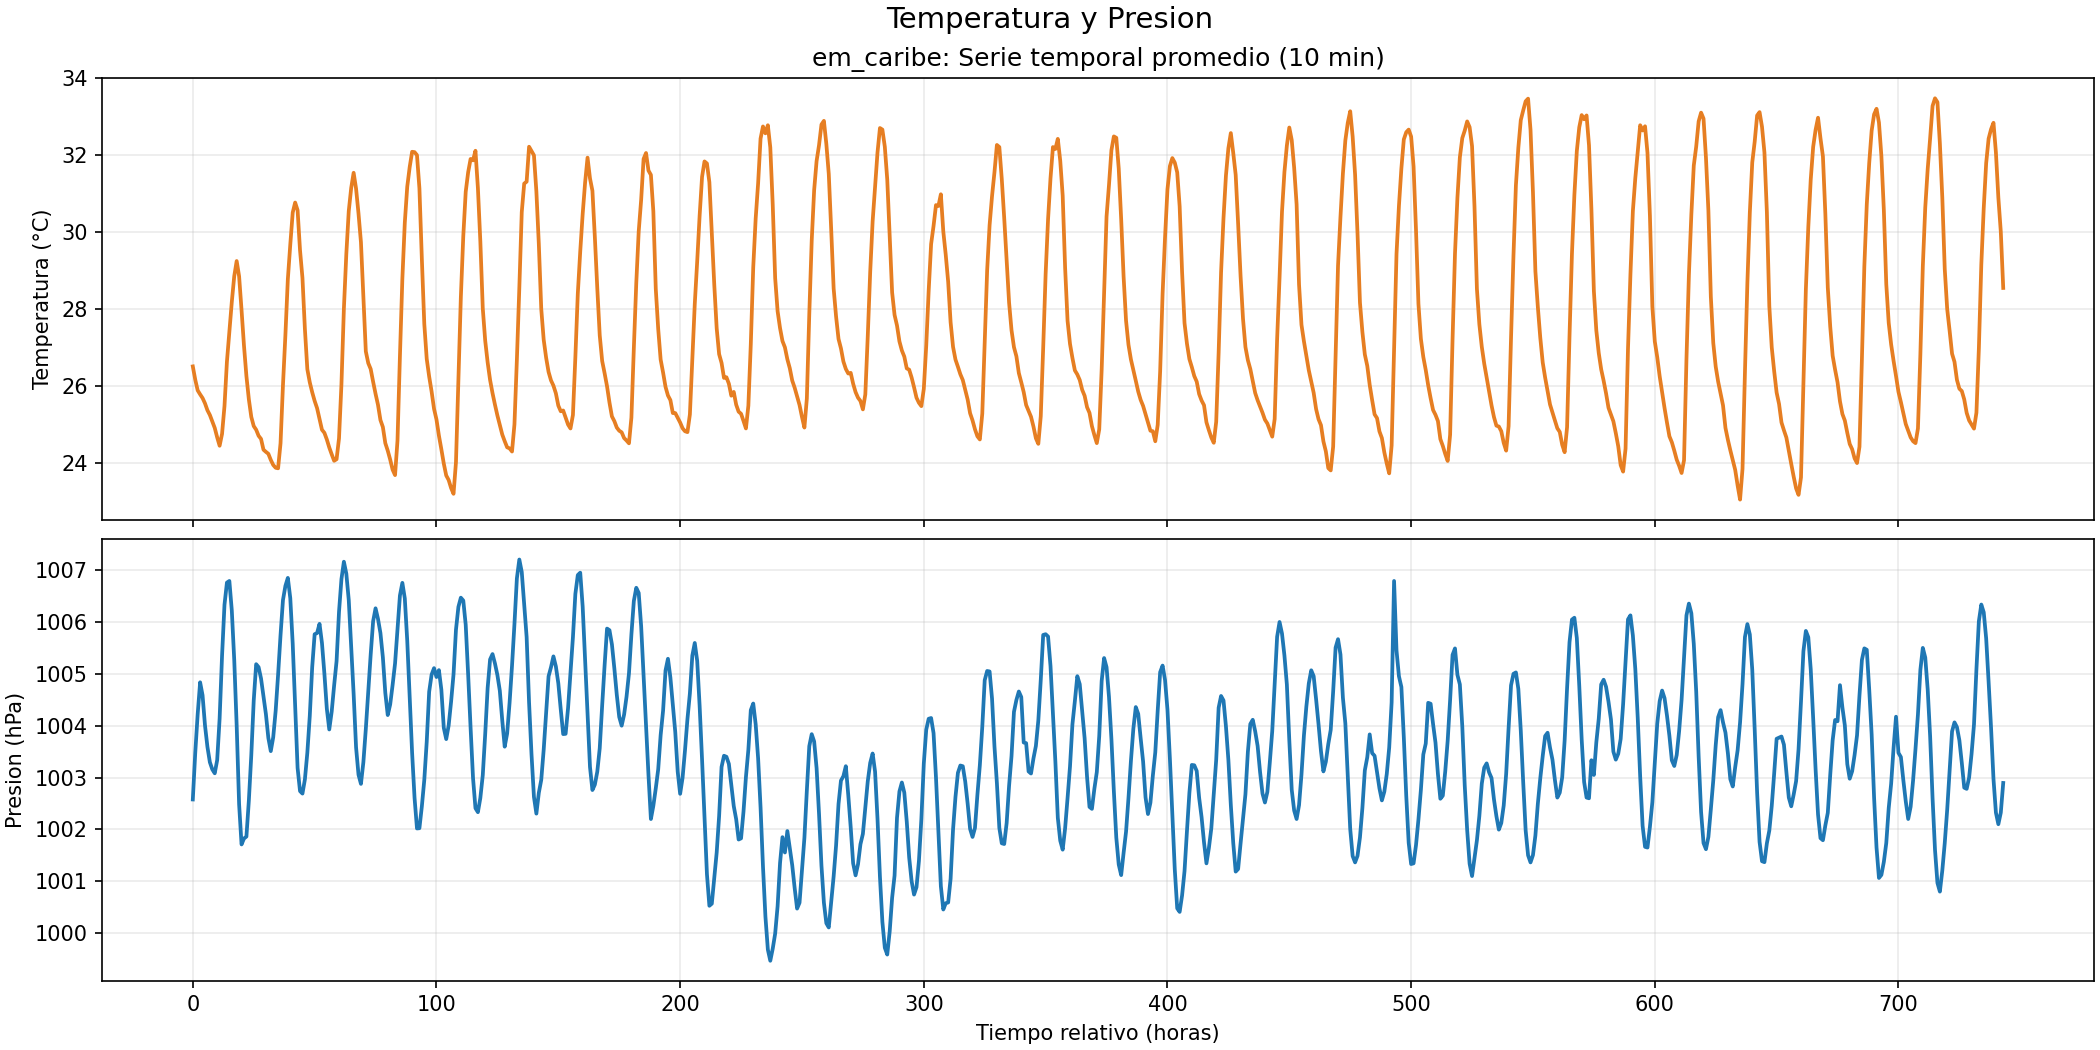
\includegraphics[width=0.80\textwidth]{Imagenes/descripcion_datos/em_caribe_temp_presion_time_series.png}
\caption{Serie temporal de temperatura y presion del conjunto Caribe para diciembre de 2025. Se evidencia variabilidad temporal apreciable en el periodo de entrenamiento.}
\label{fig:serie_temporal_datos_caribe}
\end{figure}

Como complemento de la caracterizacion temporal, la Figura~\ref{fig:serie_temporal_ux_uy_caribe} presenta la evolucion de las componentes del viento $u_x$ y $u_y$ en el periodo analizado. Esta evidencia permite contextualizar la variabilidad dinamica de las variables de salida principales del modelo.

\begin{figure}[H]
\centering
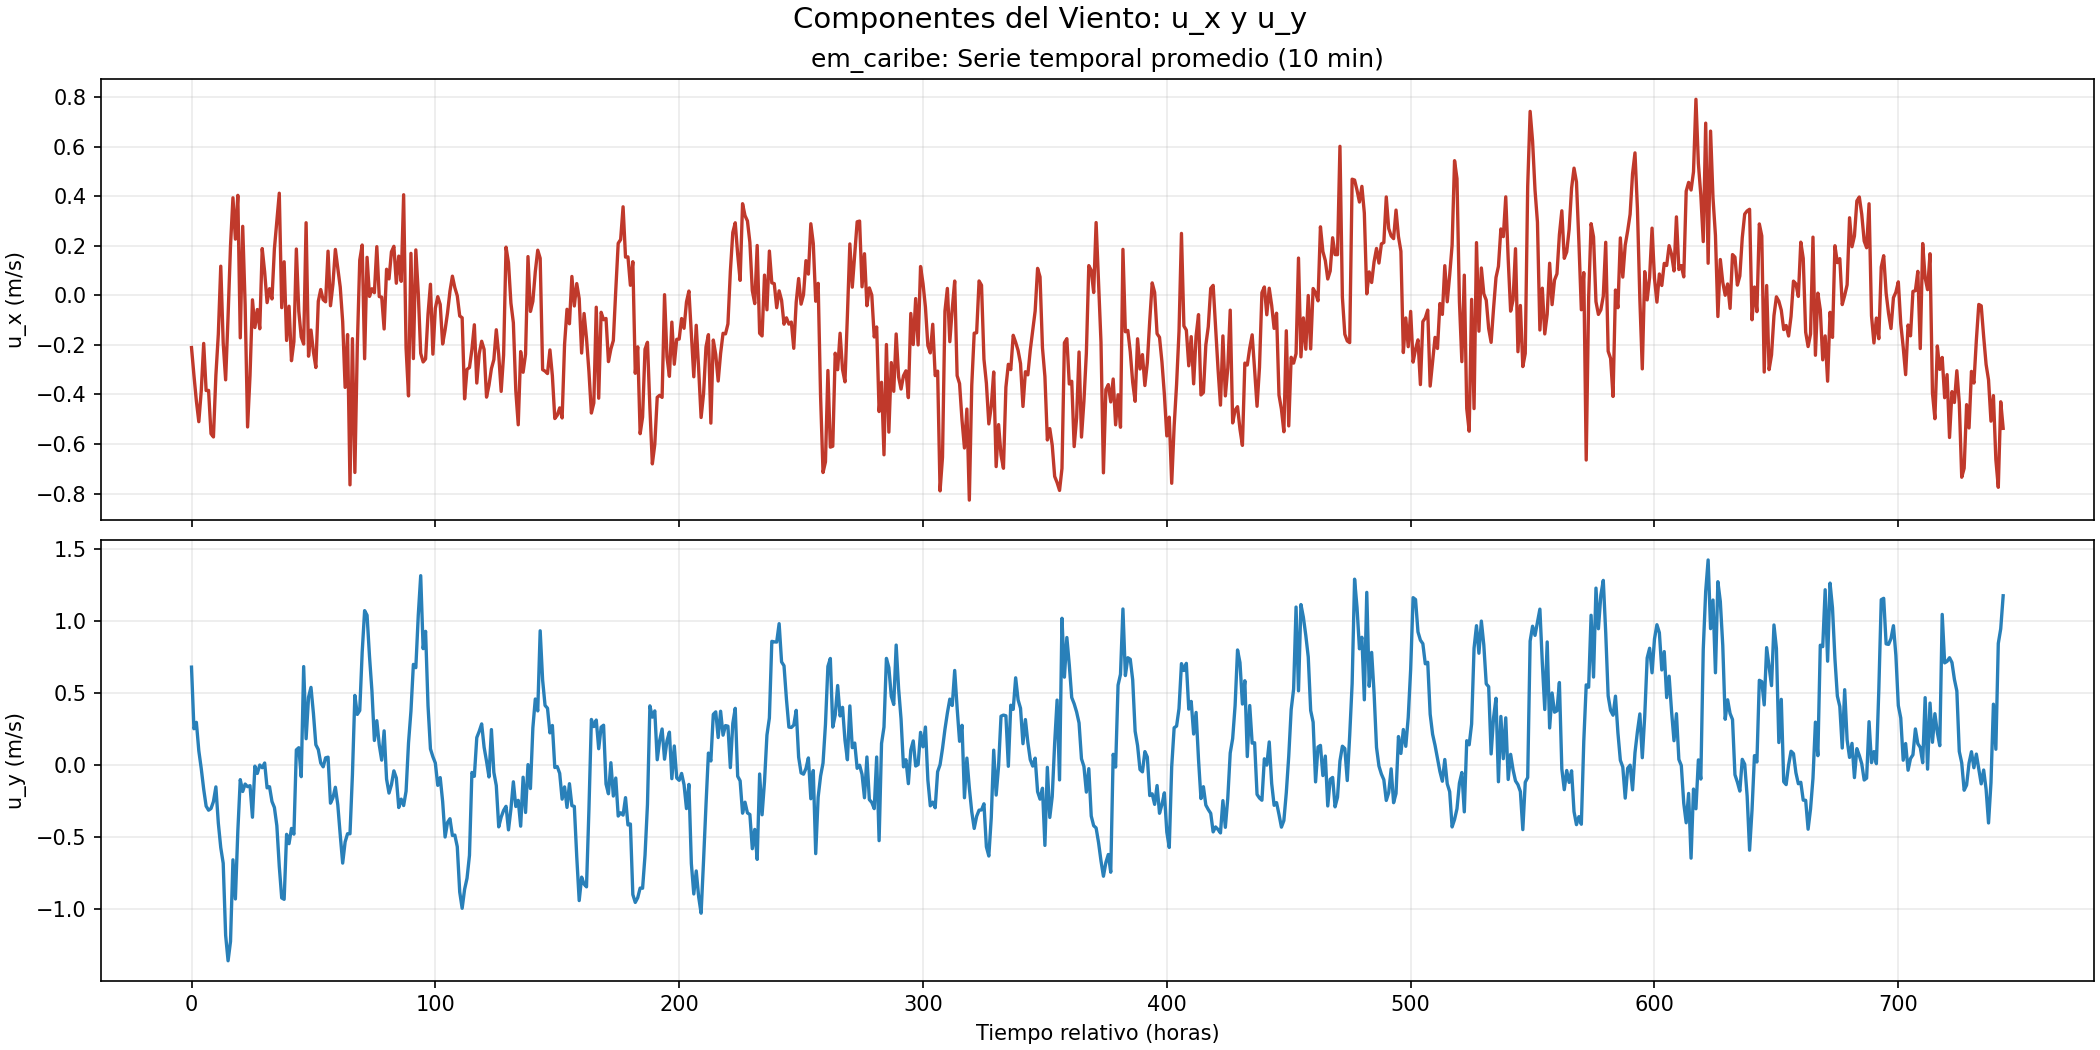
\includegraphics[width=0.90\textwidth]{Imagenes/descripcion_datos/em_caribe_ux_uy_time_series.png}
\caption{Serie temporal promedio de las componentes del viento $u_x$ y $u_y$ para el conjunto Caribe durante diciembre de 2025. La figura complementa la caracterizacion temporal de las variables meteorologicas empleadas en el estudio.}
\label{fig:serie_temporal_ux_uy_caribe}
\end{figure}

La Figura~\ref{fig:hist_temp_caribe} presenta la distribucion de temperatura del conjunto analizado. Este resumen descriptivo complementa la configuracion experimental al mostrar la concentracion de observaciones en un rango principal y la presencia de valores menos frecuentes en los extremos, condicion que es relevante para interpretar el comportamiento de la funcion de perdida durante el entrenamiento.

\begin{figure}[H]
\centering
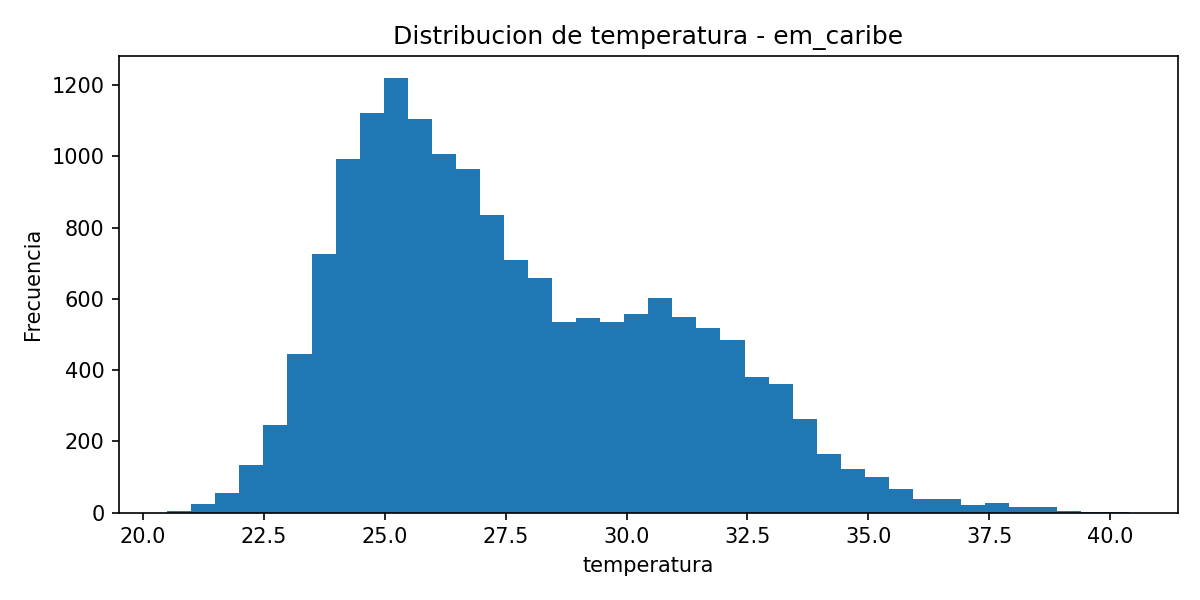
\includegraphics[width=0.80\textwidth]{Imagenes/descripcion_datos/em_caribe_temp_hist.png}
\caption{Histograma de temperatura del conjunto Caribe para diciembre de 2025. La figura se usa como apoyo descriptivo para contextualizar la distribucion de una variable de entrada clave del modelo.}
\label{fig:hist_temp_caribe}
\end{figure}

\section{Tabla maestra de experimentos evaluados}

La Tabla~\ref{tab:maestra_resultados} resume las corridas evaluadas de forma reproducible con métricas de la época 2.000. Cada fila corresponde a una configuración única de $(R, \lambda)$, con sus respectivos errores observacionales y residual físico.

\begin{table}[H]
\centering
\caption{Resultados consolidados de experimentos evaluados a época 2.000}
\label{tab:maestra_resultados}
\begin{tabular}{lcccccccc}
\hline
Modelo & $R$ & $\lambda$ & Reg./est. & Loss final & $\text{MSE}_{u_x}$ & $\text{MSE}_{u_y}$ & $\text{MSE}_{p}$ & $\mathcal{R}_{\text{NS}}$ \\
\hline
\texttt{todos\_R01\_L5} & 0,1 & 5 & $\sim744$ & 0,9261 & 0,4633 & 0,4347 & 1,3688 & \textbf{0,01273} \\
\texttt{300xest\_R01\_L5} & 0,1 & 5 & 300 & 1,1207 & 0,4689 & 0,4647 & 1,6220 & 0,03682 \\
\texttt{300xest\_R04\_L1} & 0,4 & 1 & 300 & 1,0575 & 0,5059 & 0,5085 & 1,5720 & 0,24141 \\
\texttt{300xest\_R01\_L1} & 0,1 & 1 & 300 & 1,1380 & 0,4806 & 0,4756 & 1,6477 & 0,20107 \\
\texttt{300xest\_R04\_L10} & 0,4 & 10 & 300 & 1,0859 & 0,5220 & 0,5224 & 1,6185 & 0,02242 \\
\texttt{300xest\_R01\_L10} & 0,1 & 10 & 300 & 1,1624 & 0,4919 & 0,4966 & 1,6906 & 0,02318 \\
\texttt{300xest\_R04\_L3} & 0,4 & 3 & 300 & 1,2357 & 0,6150 & 0,6274 & 1,8239 & 0,05974 \\
\texttt{300xest\_R01\_L3} & 0,1 & 3 & 300 & 1,6271 & 0,6921 & 0,6847 & 2,3727 & 0,11364 \\
\texttt{300xest\_R04\_L5} & 0,4 & 5 & 300 & 1,6203 & 0,7710 & 0,7817 & 2,4111 & 0,07074 \\
\hline
\end{tabular}
\end{table}

\noindent\textit{Nota:} La corrida extendida con restriccion suave de rango (\texttt{todosreg\_R01\_L5\_rangeL05}) se reporta de forma explicita en la Subseccion de efecto de la restriccion suave de rango, dentro de este mismo capitulo.

El mejor desempeño global se obtuvo con la corrida \texttt{todos\_R01\_L5}, que utiliza la totalidad de los datos disponibles (aproximadamente 744 registros por estación) con resolución de malla R = 0,1° y peso físico $\lambda = 5$. Esta configuración alcanza simultáneamente el menor error observacional promedio (0,7556) y el menor residual de Navier-Stokes (0,01273) entre todos los experimentos evaluados.

\section{Ranking por error observacional promedio}

Se utilizo el criterio:

\[
\bar{MSE}_{obs}=\frac{\text{MSE}_{u_x}+\text{MSE}_{u_y}+\text{MSE}_{p}}{3}
\]

La Tabla~\ref{tab:ranking_obs} presenta el ranking consolidado.

\begin{table}[H]
\centering
\caption{Ranking por error observacional promedio}
\label{tab:ranking_obs}
\begin{tabular}{clcc}
\hline
Pos. & Modelo & $\bar{MSE}_{obs}$ & Residual NS \\
\hline
1 & \texttt{todos\_R01\_L5} & 0,75559 & 0,01273 \\
2 & \texttt{300xest\_R01\_L5} & 0,85185 & 0,03682 \\
3 & \texttt{300xest\_R04\_L1} & 0,86216 & 0,24141 \\
4 & \texttt{300xest\_R01\_L1} & 0,86796 & 0,20107 \\
5 & \texttt{300xest\_R04\_L10} & 0,88765 & 0,02242 \\
6 & \texttt{300xest\_R01\_L10} & 0,89305 & 0,02318 \\
7 & \texttt{300xest\_R04\_L3} & 1,02208 & 0,05974 \\
8 & \texttt{300xest\_R01\_L3} & 1,24982 & 0,11364 \\
9 & \texttt{300xest\_R04\_L5} & 1,32126 & 0,07074 \\
\hline
\end{tabular}
\end{table}

\section{Analisis por factores}

\subsection{Efecto de \texorpdfstring{$\lambda$ en $R=0{,}1^{\circ}$}{lambda en R=0,1 grados} (resolución fina)}

En el bloque de malla fina con 91.200 puntos de colocación, el efecto del peso físico $\lambda$ presenta un comportamiento no monótono:

\begin{table}[H]
\centering
\begin{tabular}{cccc}
\hline
$\lambda$ & $\overline{\text{MSE}}_{\text{obs}}$ & $\mathcal{R}_{\text{NS}}$ & Caracterización \\
\hline
1 & 0,86796 & 0,20107 & Balance moderado, residual alto \\
3 & 1,24982 & 0,11364 & Peor resultado del bloque \\
5 & \textbf{0,85185} & \textbf{0,03682} & \textbf{Mejor equilibrio obs-físico} \\
10 & 0,89305 & 0,02318 & Residual mínimo, velocidades degradadas \\
\hline
\end{tabular}
\caption{Efecto de $\lambda$ en $R=0{,}1^{\circ}$: evolución de error observacional y residual físico.}
\label{tab:lambda_r01}
\end{table}

El valor $\lambda = 5$ emerge como óptimo en este bloque, equilibrando ajuste observacional y satisfacción de las restricciones físicas. Notablemente, $\lambda = 3$ produce degradación sistemática en ambos criterios.

\subsection{Efecto de \texorpdfstring{$\lambda$ en $R=0{,}4^{\circ}$}{lambda en R=0,4 grados} (resolución gruesa)}

En el bloque de malla gruesa \((R=0{,}4^{\circ})\), con 13.200 puntos de colocación, se observa un compromiso claro entre desempeño observacional y cumplimiento físico: $\lambda=1$ logra el mejor ajuste observacional $\left(\overline{\text{MSE}}_{\text{obs}}=0{,}86216\right)$ pero con residual elevado $\left(\mathcal{R}_{\text{NS}}=0{,}24141\right)$, mientras que $\lambda=10$ obtiene el residual mínimo del bloque $\left(\mathcal{R}_{\text{NS}}=0{,}02242\right)$ con una pérdida moderada en el ajuste observacional $\left(\overline{\text{MSE}}_{\text{obs}}=0{,}88765\right)$; por su parte, $\lambda=3$ presenta comportamiento intermedio $\left(\overline{\text{MSE}}_{\text{obs}}=1{,}02208,\ \mathcal{R}_{\text{NS}}=0{,}05974\right)$ y $\lambda=5$ concentra el peor desempeño observacional del bloque $\left(\overline{\text{MSE}}_{\text{obs}}=1{,}32126,\ \mathcal{R}_{\text{NS}}=0{,}07074\right)$, lo que confirma que en esta resolución no existe un valor único dominante para ambos criterios y que el incremento de $\lambda$ favorece la restricción física en detrimento parcial del ajuste a observaciones.

\subsection{Patrón crítico: insuficiencia de \texorpdfstring{$\lambda = 3$}{lambda = 3}}

Un hallazgo metodológico relevante es que $\lambda = 3$ presenta desempeño consistentemente desfavorable en ambas resoluciones de malla. La Tabla~\ref{tab:lambda_r01} y los resultados descritos en la sección anterior muestran que este valor específico genera una tensión desequilibrada entre objetivos observacional y físico, resultando en errores superiores a las alternativas adyacentes ($\lambda = 1$ y $\lambda = 5$).

\subsection{Efecto de la resolucion de malla}

Comparando pares equivalentes con $\lambda$ fijo pero $R$ diferente:

\begin{table}[H]
\centering
\begin{tabular}{ccccc}
\hline
$\lambda$ & $\overline{\text{MSE}}_{\text{obs}}$ R=0,1 & $\overline{\text{MSE}}_{\text{obs}}$ R=0,4 & Diferencia & Mejor R \\
\hline
1 & 0,86796 & 0,86216 & -0,0058 (marginal) & 0,4 \\
3 & 1,24982 & 1,02208 & -0,2277 (marcado) & 0,4 \\
5 & 0,85185 & 1,32126 & +0,4694 (marcado) & \textbf{0,1} \\
10 & 0,89305 & 0,88765 & -0,0054 (marginal) & 0,4 \\
\hline
\end{tabular}
\caption{Comparación de resoluciones: R = 0,4° domina en $\lambda \in \{1, 3, 10\}$, pero R = 0,1° es superior en $\lambda = 5$.}
\label{tab:efecto_resolucion}
\end{table}

Este resultado sugiere que la densidad de puntos de colocación modula la efectividad del peso físico. Una malla más fina (R = 0,1°) requiere un $\lambda$ mayor para controlar el comportamiento sobre los puntos adicionales de colocación; con $\lambda$ bajo, los puntos extras quedan infrautilizados.

\subsection{Efecto del volumen de datos}

La corrida final utilizó la totalidad de los registros disponibles, manteniendo la configuración óptima identificada en el barrido (R = 0,1°, $\lambda = 5$). Con la misma arquitectura y configuración de entrenamiento, el incremento de datos produjo mejoras sustanciales:

\begin{table}[H]
\centering
\begin{tabular}{lccc}
\hline
Configuración & Registros totales & $\overline{\text{MSE}}_{\text{obs}}$ & $\mathcal{R}_{\text{NS}}$ \\
\hline
\texttt{300xest\_R01\_L5} & 5.400 & 0,85185 & 0,03682 \\
\texttt{todos\_R01\_L5} & 13.392 & 0,75559 & 0,01273 \\
\hline
Mejora (reducción \%) & 2,48× más & -11,3\% & -65,4\% \\
\hline
\end{tabular}
\caption{Impacto del volumen de datos: con 744 registros/estación (~13.392 en total) frente a 300 registros/estación (5.400 total), manteniendo R = 0,1° y $\lambda = 5$.}
\label{tab:efecto_volumen}
\end{table}

El incremento de 2,48× en el volumen de datos resultó en reducción del 11,3\% del error observacional promedio y del 65,4\% del residual de Navier-Stokes. Este resultado indica que el modelo PINN aún operaba en régimen de datos limitados durante el barrido, y que la cobertura temporal ampliada es una palanca efectiva de mejora sin cambios arquitecturales.

\subsection{Efecto de la restriccion suave de rango}

Como extension metodologica del estudio, se evaluo una corrida adicional con restriccion suave de rango sobre la configuracion de referencia $R=0{,}1^\circ$, $\lambda=5$, denominada \texttt{todosreg\_R01\_L5\_rangeL05}. Esta variante incorporo cuantiles robustos, penalizacion softplus y una rampa lineal para el peso $\lambda_R$ dentro de la funcion de perdida extendida.

La Tabla~\ref{tab:range_loss_comp} compara tres escenarios con arquitectura comun y la misma pareja $(R,\lambda)=(0{,}1,5)$, diferenciados por volumen de datos y por la activacion del mecanismo de rango.

\begin{table}[H]
\centering
\begin{tabular}{lccc}
\hline
Experimento & Registros totales & Mecanismo de rango & Loss final \\
\hline
\texttt{300xest\_R01\_L5} & 5.400 & No & 1,117 \\
\texttt{todos\_R01\_L5} & 13.392 & No & 0,926 \\
\texttt{todosreg\_R01\_L5\_rangeL05} & 13.392 & Si & \textbf{0,638} \\
\hline
\end{tabular}
\caption{Comparacion de perdida final a epoca 2.000 en escenarios de referencia con y sin restriccion suave de rango.}
\label{tab:range_loss_comp}
\end{table}

Para verificar si la reduccion de la perdida total se traduce en un beneficio genuino sobre el ajuste observacional y no solamente en la satisfaccion del termino de penalizacion de rango, se evaluaron las metricas desagregadas del modelo de referencia frente al modelo con restriccion de rango. La Tabla~\ref{tab:range_metricas_comp} presenta esta comparacion.

\begin{table}[H]
\centering
\caption{Metricas comparativas entre el modelo base y el modelo con restriccion de rango}
\label{tab:range_metricas_comp}
\begin{tabular}{lccc}
\hline
Metrica & \texttt{todos\_R01\_L5} & \texttt{todosreg\_R01\_L5\_rangeL05} & Variacion \\
\hline
$\text{MSE}_{u_x}$ & 0,4633 & 0,3799 & $-18{,}0\%$ \\
$\text{MSE}_{u_y}$ & 0,4347 & 0,3775 & $-13{,}2\%$ \\
$\text{MSE}_{p}$ & 1,3688 & 0,9875 & $-27{,}9\%$ \\
$\mathcal{R}_{\text{NS}}$ & 0,01273 & 0,01534 & $+20{,}5\%$ \\
Loss total & 0,926 & \textbf{0,638} & $-31{,}1\%$ \\
\hline
\end{tabular}
\end{table}

\noindent\textit{Nota: variables en unidades normalizadas. MSE calculado sobre los puntos de las estaciones; $\mathcal{R}_{\text{NS}}$ sobre los puntos de colocacion.}

Los resultados indican que la incorporacion de la restriccion de rango produce una mejora real en el ajuste observacional: el MSE disminuye entre 13\,\% y 28\,\% para las tres variables de salida con respecto al modelo base. Esta mejora no es un artefacto de la funcion de perdida: el termino de penalizacion de rango actua sobre los puntos de la malla, no sobre los puntos de las estaciones donde se calcula el MSE. La reduccion del MSE observacional refleja por tanto una regularizacion implicita del campo de prediccion: al forzar que las predicciones en zonas no observadas permanezcan dentro de rangos plausibles, el modelo evita soluciones patologicas que propaguen errores hacia las regiones con estaciones.

No obstante, la restriccion de rango presenta dos efectos secundarios que deben considerarse. Primero, el residual de Navier-Stokes aumenta levemente ($\mathcal{R}_{\text{NS}}$: 0,01273 $\to$ 0,01534, $+20{,}5$\,\%), lo que indica que la penalizacion de rango compite parcialmente con la restriccion fisica durante el entrenamiento. Segundo, el porcentaje de predicciones fuera de rango en la malla completa permanece elevado para las componentes de velocidad ($\text{FOR}_{u} = 64{,}35$\,\%, $\text{FOR}_{v} = 48{,}09$\,\%), lo que sugiere que la red no alcanza la cobertura completa del rango en las 2.000 epocas evaluadas. La presion, en cambio, logra compliance casi total ($\text{FOR}_{p} = 0{,}28$\,\%). Este comportamiento asimetrico puede deberse a la mayor variabilidad espacial de las componentes de velocidad o a que el valor $\lambda_{R,\max} = 0{,}50$ no es suficiente para reducir FOR en velocidades dentro del horizonte de entrenamiento disponible.

En conjunto, la restriccion de rango mejora el ajuste observacional y reduce la perdida total, pero la elevada FOR en velocidades indica que el experimento no ha convergido completamente hacia el cumplimiento de la restriccion. La optimizacion de $\lambda_{R,\max}$ y del numero de epocas queda como linea de trabajo futuro.

\begin{figure}[H]
\centering
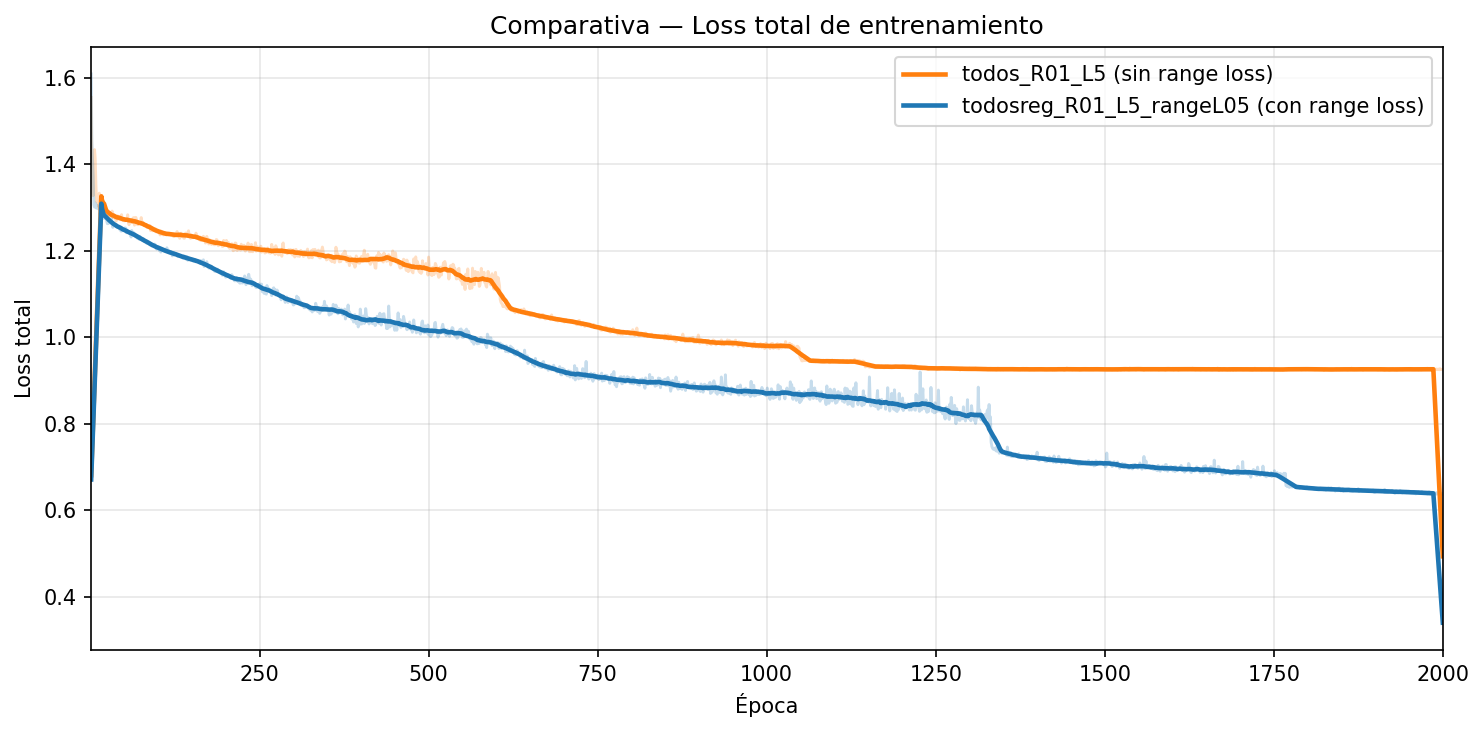
\includegraphics[width=0.92\textwidth]{Imagenes/rango/01_loss_total_comparativa.png}
\caption{Comparacion de la perdida total durante el entrenamiento para escenarios de referencia con y sin restriccion suave de rango.}
\label{fig:range_loss_total_comp}
\end{figure}

Como resultado final del entrenamiento con restriccion suave de rango, las Figuras~\ref{fig:range_campo_u}, \ref{fig:range_campo_v} y \ref{fig:range_campo_p} presentan los campos predichos para las componentes de velocidad y la presion en la corrida \texttt{todosreg\_R01\_L5\_rangeL05}.

\begin{figure}[H]
\centering
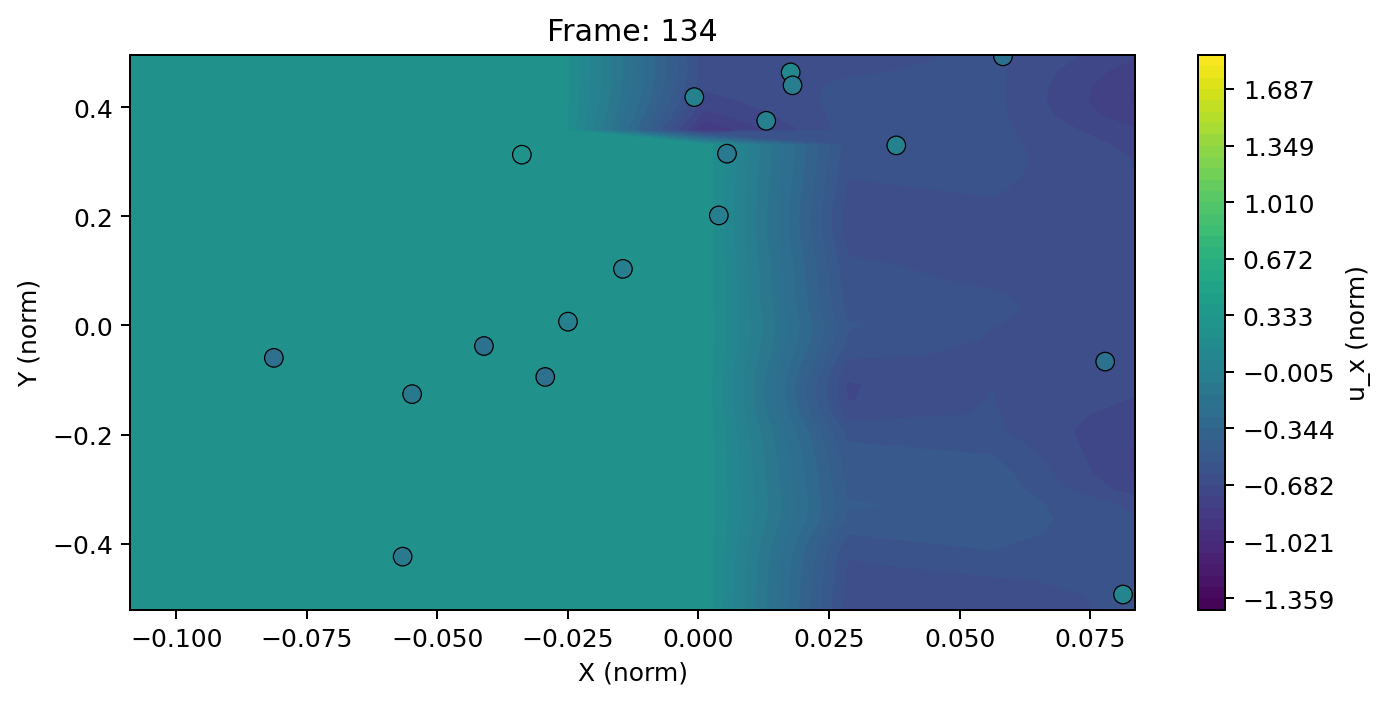
\includegraphics[width=0.92\textwidth]{Imagenes/rango/pinn_caribe_excl4_todosreg_r01_l5_rangel05_epoca_2000_frame_min_loss_general_u_t134.png}
\caption{Campo predicho final de $u$ para la corrida \texttt{todosreg\_R01\_L5\_rangeL05}.}
\label{fig:range_campo_u}
\end{figure}

\begin{figure}[H]
\centering
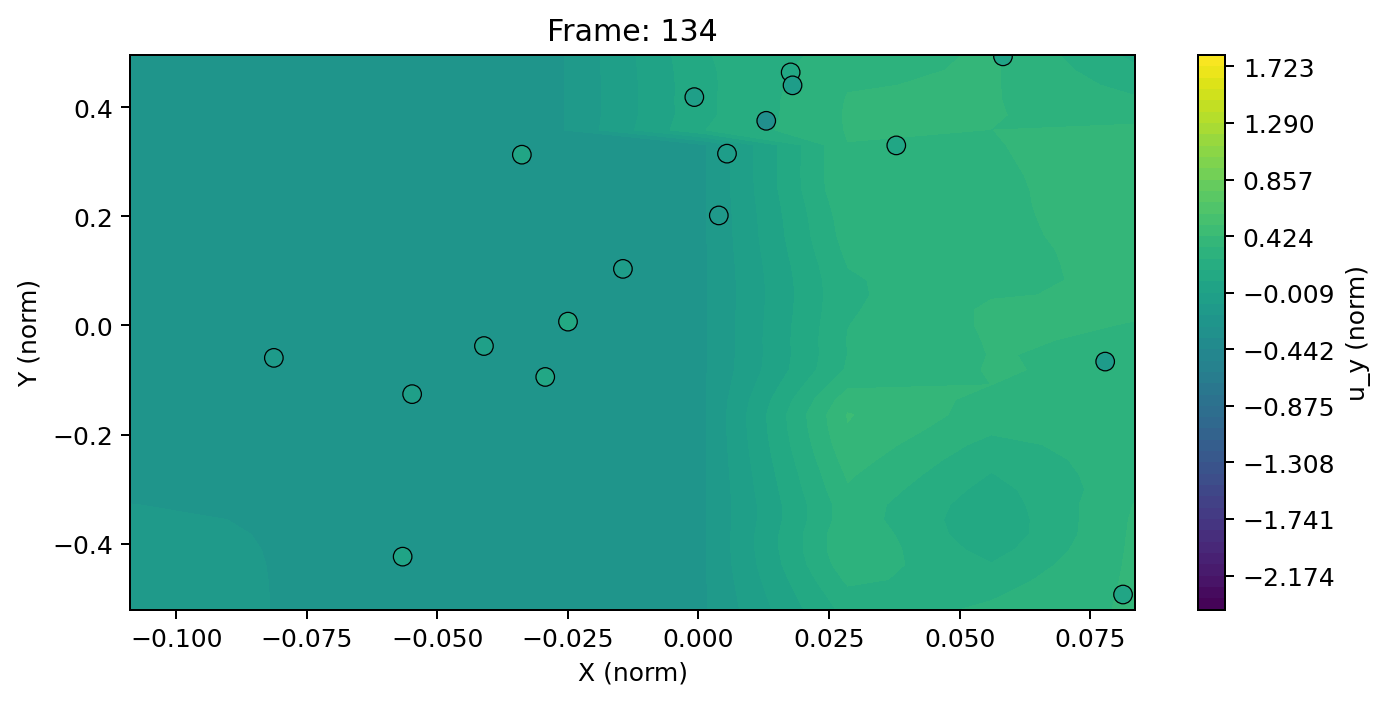
\includegraphics[width=0.92\textwidth]{Imagenes/rango/pinn_caribe_excl4_todosreg_r01_l5_rangel05_epoca_2000_frame_min_loss_general_v_t134.png}
\caption{Campo predicho final de $v$ para la corrida \texttt{todosreg\_R01\_L5\_rangeL05}.}
\label{fig:range_campo_v}
\end{figure}

\begin{figure}[H]
\centering
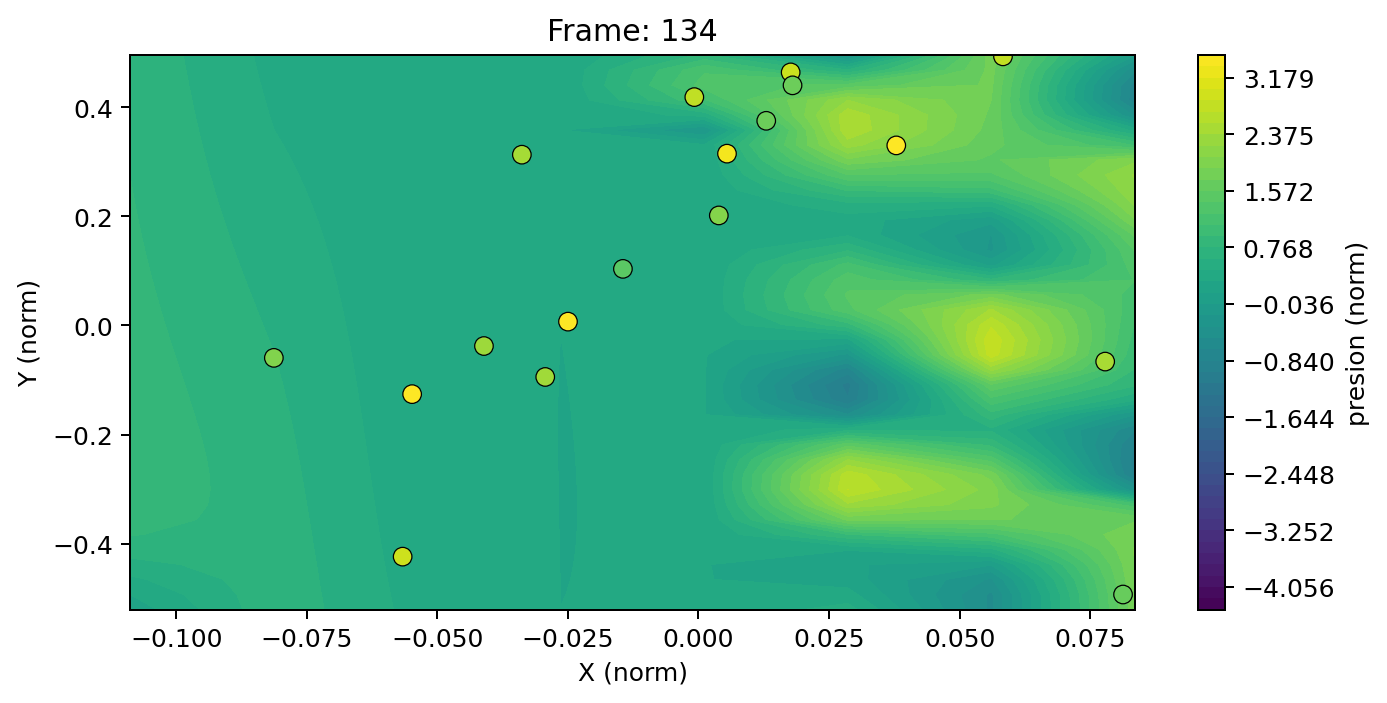
\includegraphics[width=0.92\textwidth]{Imagenes/rango/pinn_caribe_excl4_todosreg_r01_l5_rangel05_epoca_2000_frame_min_loss_general_p_t134.png}
\caption{Campo predicho final de $p$ para la corrida \texttt{todosreg\_R01\_L5\_rangeL05}.}
\label{fig:range_campo_p}
\end{figure}

\begin{figure}[H]
\centering
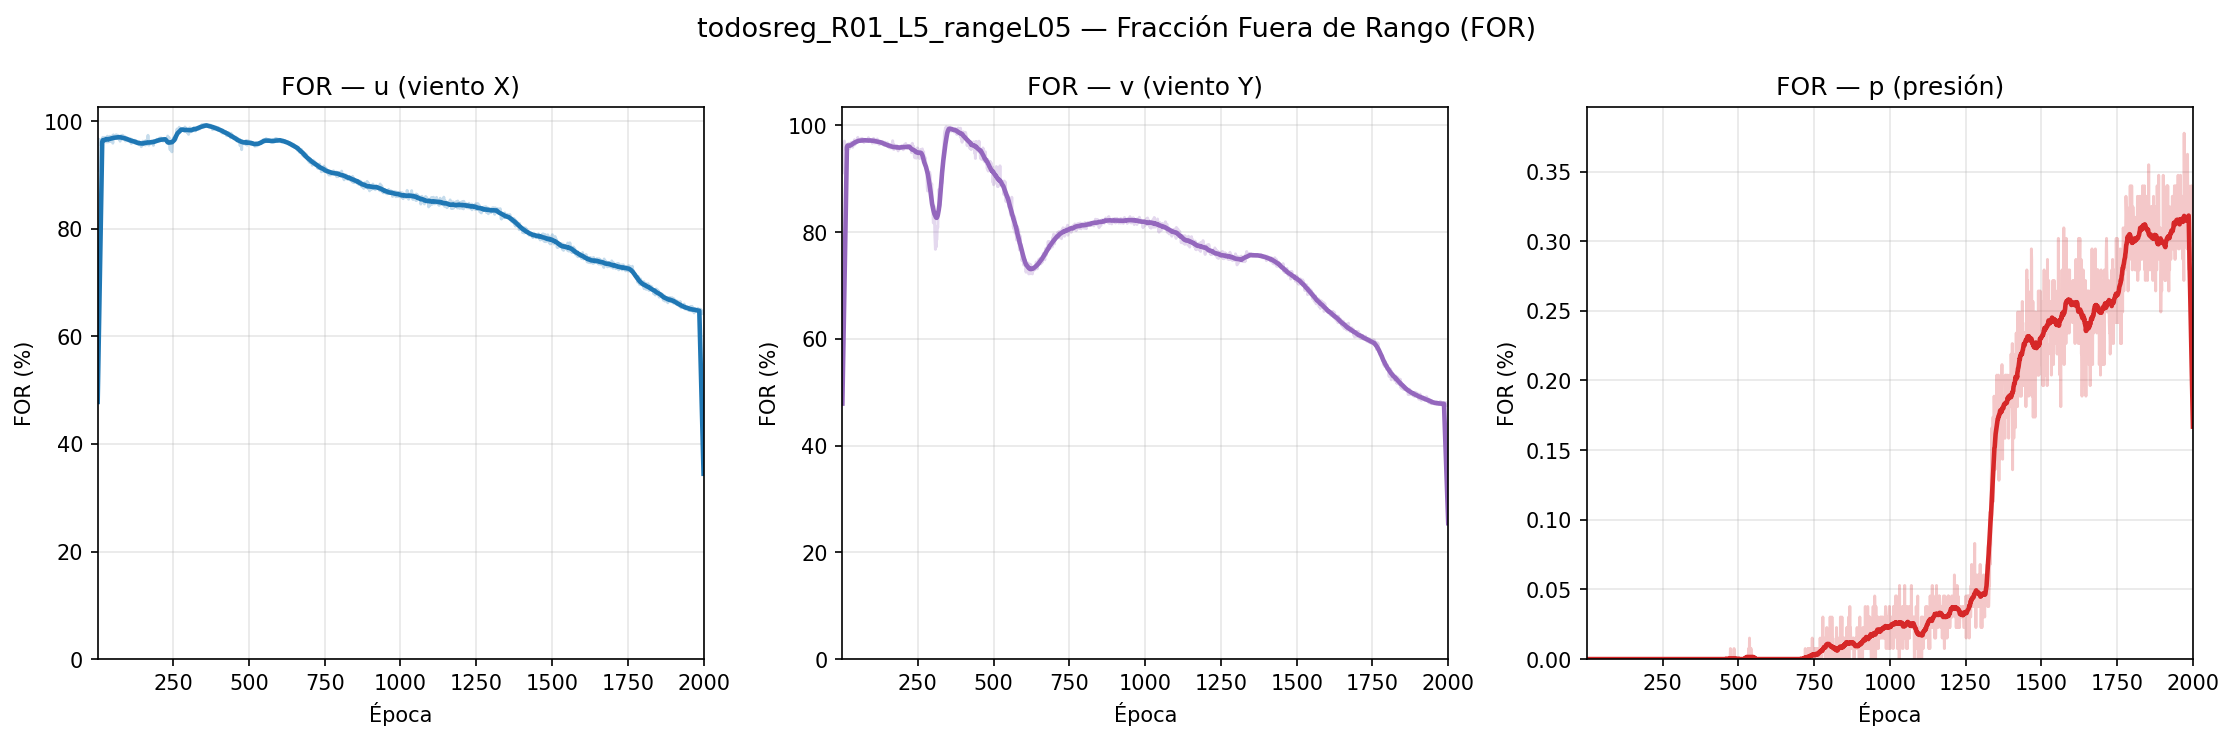
\includegraphics[width=0.92\textwidth]{Imagenes/rango/05_for_metricas.png}
\caption{Evolucion de la metrica FOR para las variables de salida en la corrida con restriccion suave de rango.}
\label{fig:range_for_metricas}
\end{figure}

\section{Validación fuera de muestra: generalización temporal}

Para evaluar la capacidad de generalización del modelo a condiciones temporales no vistas
durante el entrenamiento, se realizó una partición temporal del conjunto de datos:
los días 1 a 20 de diciembre de 2025 (8.574 registros) se utilizaron para el entrenamiento,
y los días 21 a 31 (4.818 registros) constituyeron el conjunto de prueba independiente.
Se entrenó el modelo con la configuración de referencia ($R = 0{,}1^{\circ}$, $\lambda = 5{,}0$,
2.000 épocas, todas las estaciones activas) y se evaluaron las métricas $\text{MSE}_{\text{obs}}$
y $\mathcal{R}_{\text{NS}}$ sobre el conjunto de prueba una vez completado el entrenamiento.
La Tabla~\ref{tab:validacion_prueba} compara las métricas obtenidas en entrenamiento y en prueba.
Los valores de referencia del entrenamiento corresponden al modelo \texttt{todos\_R01\_L5}
(entrenado con los 31 días completos) y se incluyen como referencia de escala para las variables
en unidades normalizadas.

\begin{table}[H]
\centering
\caption{Comparación de métricas entre el conjunto de entrenamiento (días 1–20) y el conjunto de prueba (días 21–31) para el modelo \texttt{PINN\_caribe\_excl4\_todos\_R01\_L5\_train20d}}
\label{tab:validacion_prueba}
\begin{tabular}{lccc}
\hline
Métrica & Entrenamiento (días 1–20) & Prueba (días 21–31) & Diferencia \\
\hline
$\text{MSE}_{u_x}$ & 0{,}4633 & \textbf{0{,}4422} & $-4{,}5$\,\% \\
$\text{MSE}_{u_y}$ & 0{,}4347 & \textbf{0{,}4248} & $-2{,}3$\,\% \\
$\text{MSE}_{p}$   & 1{,}3688 & \textbf{3{,}9116} & $+185{,}8$\,\% \\
$\mathcal{R}_{\text{NS}}$ & 0{,}01273 & \textbf{0{,}03640} & $+186{,}0$\,\% \\
\hline
\end{tabular}
\end{table}

\noindent\textit{Nota: variables en unidades normalizadas. MSE calculado sobre los puntos de las
estaciones; $\mathcal{R}_{\text{NS}}$ sobre los puntos de colocación. Valores de referencia de entrenamiento tomados del modelo
\texttt{todos\_R01\_L5} (31 días completos).}

Los resultados evidencian un comportamiento diferenciado según la variable de salida.
Las componentes de velocidad del viento ($u_x$, $u_y$) muestran métricas de prueba
prácticamente idénticas a las de entrenamiento (diferencias de $-4{,}5$\,\% y $-2{,}3$\,\%
respectivamente), lo que sugiere que la restricción física de Navier-Stokes actúa como
regularizador efectivo para el campo de velocidades y permite una generalización temporal
satisfactoria a los 11 días no vistos durante el entrenamiento.

Sin embargo, el $\text{MSE}$ de presión aumenta de forma significativa en el conjunto de
prueba ($1{,}3688 \to 3{,}9116$, un incremento del $185{,}8$\,\%), indicando sobreajuste en la
variable de presión. Este comportamiento asimétrico es coherente con la naturaleza de los datos:
la presión atmosférica exhibe mayor variabilidad temporal y menor densidad observacional que las
componentes de velocidad, lo que reduce la capacidad del modelo para extrapolar su campo fuera
del período de entrenamiento. El residual de Navier-Stokes también aumenta en prueba
($0{,}01273 \to 0{,}03640$, $+186{,}0$\,\%), confirmando que las restricciones físicas aprendidas
sobre los primeros 20 días no se transfieren plenamente al período de prueba.

En conjunto, estos resultados sugieren que la PINN desarrollada tiene capacidad de
generalización temporal para el campo de viento, pero no para el campo de presión en el período
evaluado. Las predicciones de viento sobre días no vistos pueden considerarse razonablemente
confiables dentro del dominio y período estudiados, mientras que las predicciones de presión
deben interpretarse con cautela fuera del período de entrenamiento. Como líneas de mejora se
proponen: (1)~incorporar datos de presión de mayor resolución temporal, (2)~aumentar el peso
relativo de la pérdida física sobre la presión ($\lambda_p > \lambda_{\text{viento}}$),
o (3)~ampliar el período de entrenamiento a meses adicionales disponibles en el portal de
Datos Abiertos Colombia.

\section{Evidencia visual de configuraciones de referencia}

Las Figuras~\ref{fig:error_r01_l5} y~\ref{fig:mse_r01_l5} presentan el comportamiento temporal del error para \texttt{R01\_L5} (mejor corrida del bloque de 300 registros por estacion en $R=0{,}1^\circ$).

\begin{figure}[H]
\centering
\begin{subfigure}[b]{0.85\textwidth}
  \centering
  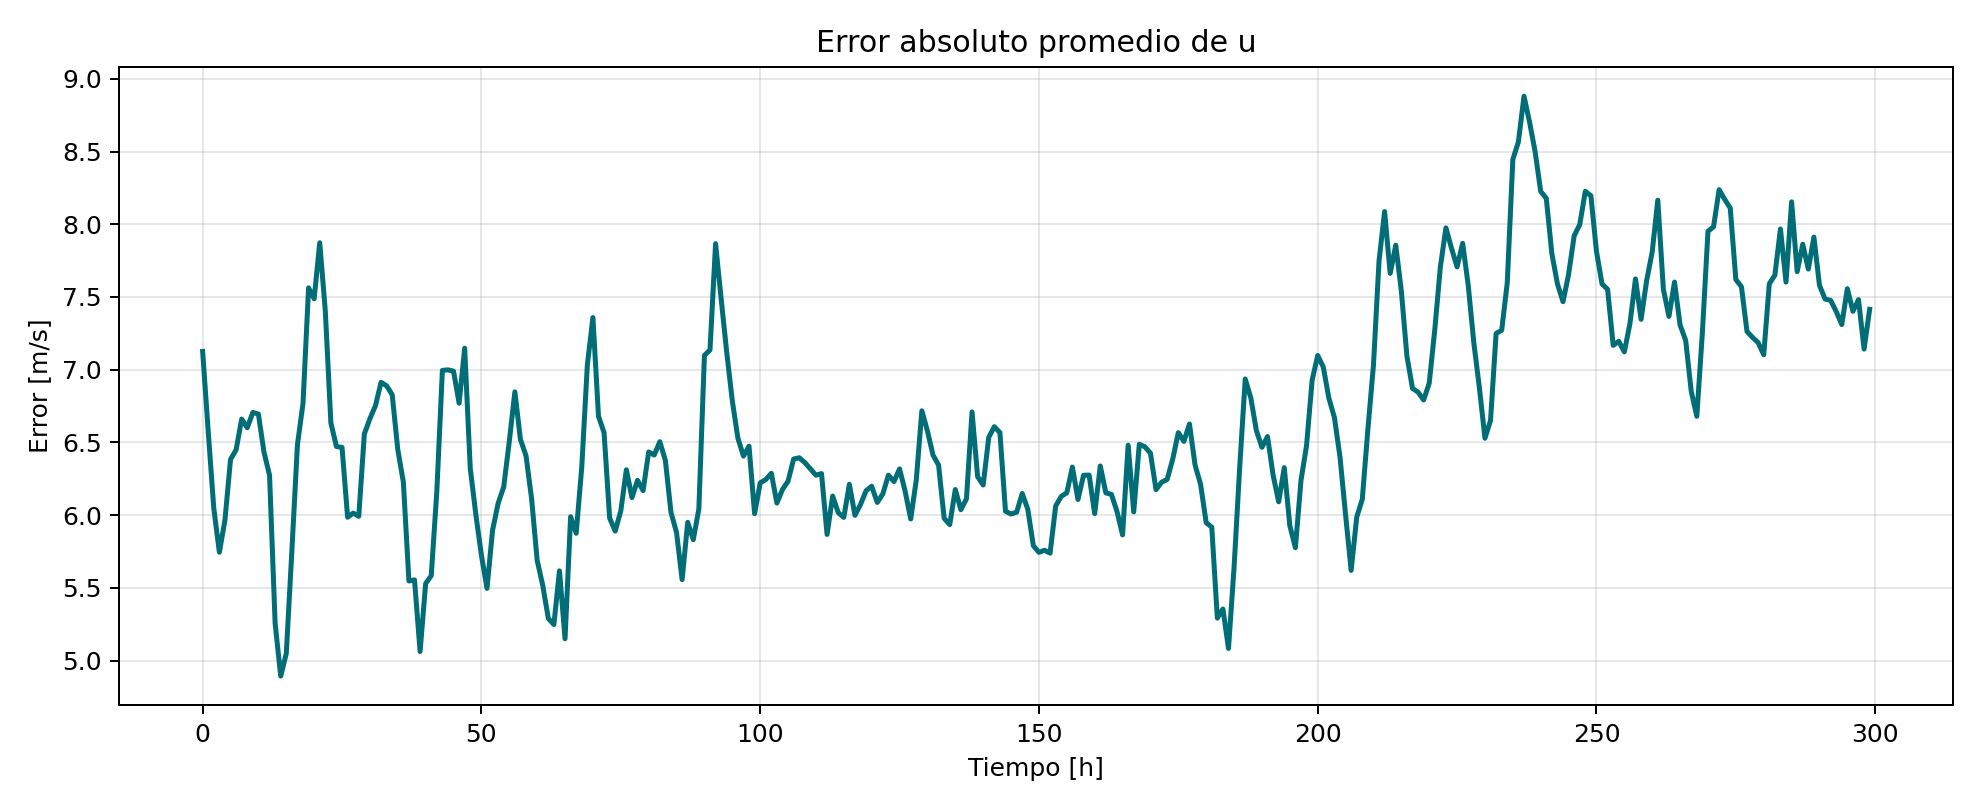
\includegraphics[width=\textwidth]{Imagenes/iter_R01/PINN_caribe_excl4_300xest_R01_L5/pinn_caribe_excl4_300xest_r01_l5_epoca_2000_error_promedio_u_tiempo.png}
  \caption{Error absoluto promedio de la componente $u$ (Este--Oeste) en m/s.}
\end{subfigure}
\par\medskip
\begin{subfigure}[b]{0.85\textwidth}
  \centering
  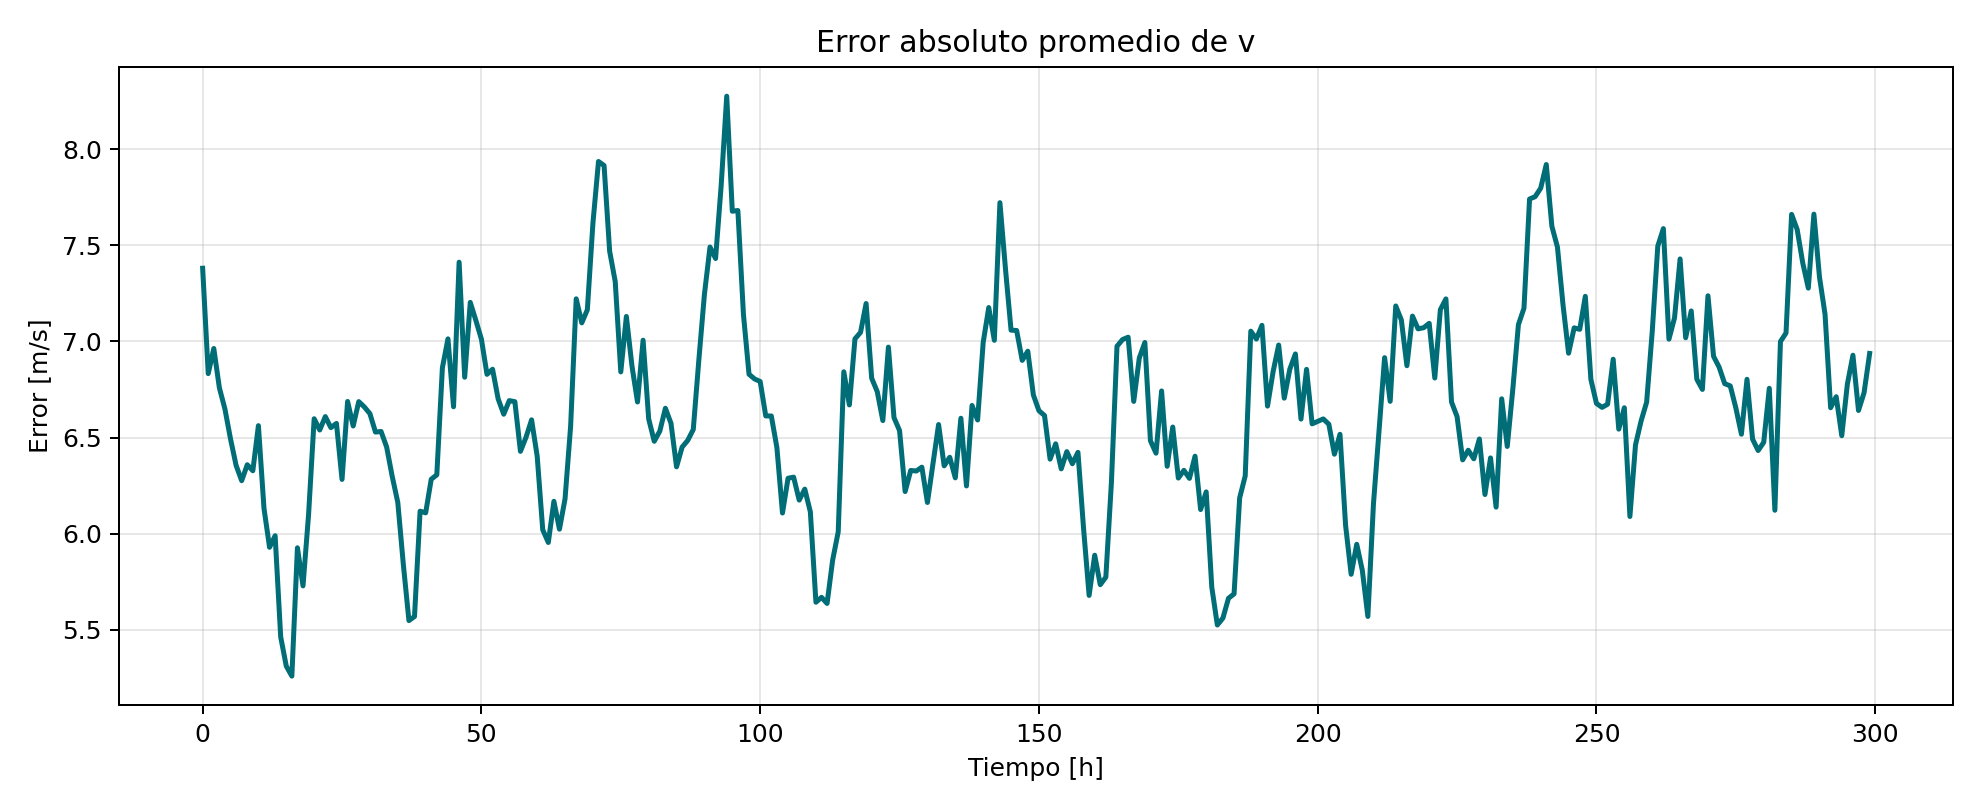
\includegraphics[width=\textwidth]{Imagenes/iter_R01/PINN_caribe_excl4_300xest_R01_L5/pinn_caribe_excl4_300xest_r01_l5_epoca_2000_error_promedio_v_tiempo.png}
  \caption{Error absoluto promedio de la componente $v$ (Norte--Sur) en m/s.}
\end{subfigure}
\par\medskip
\begin{subfigure}[b]{0.85\textwidth}
  \centering
  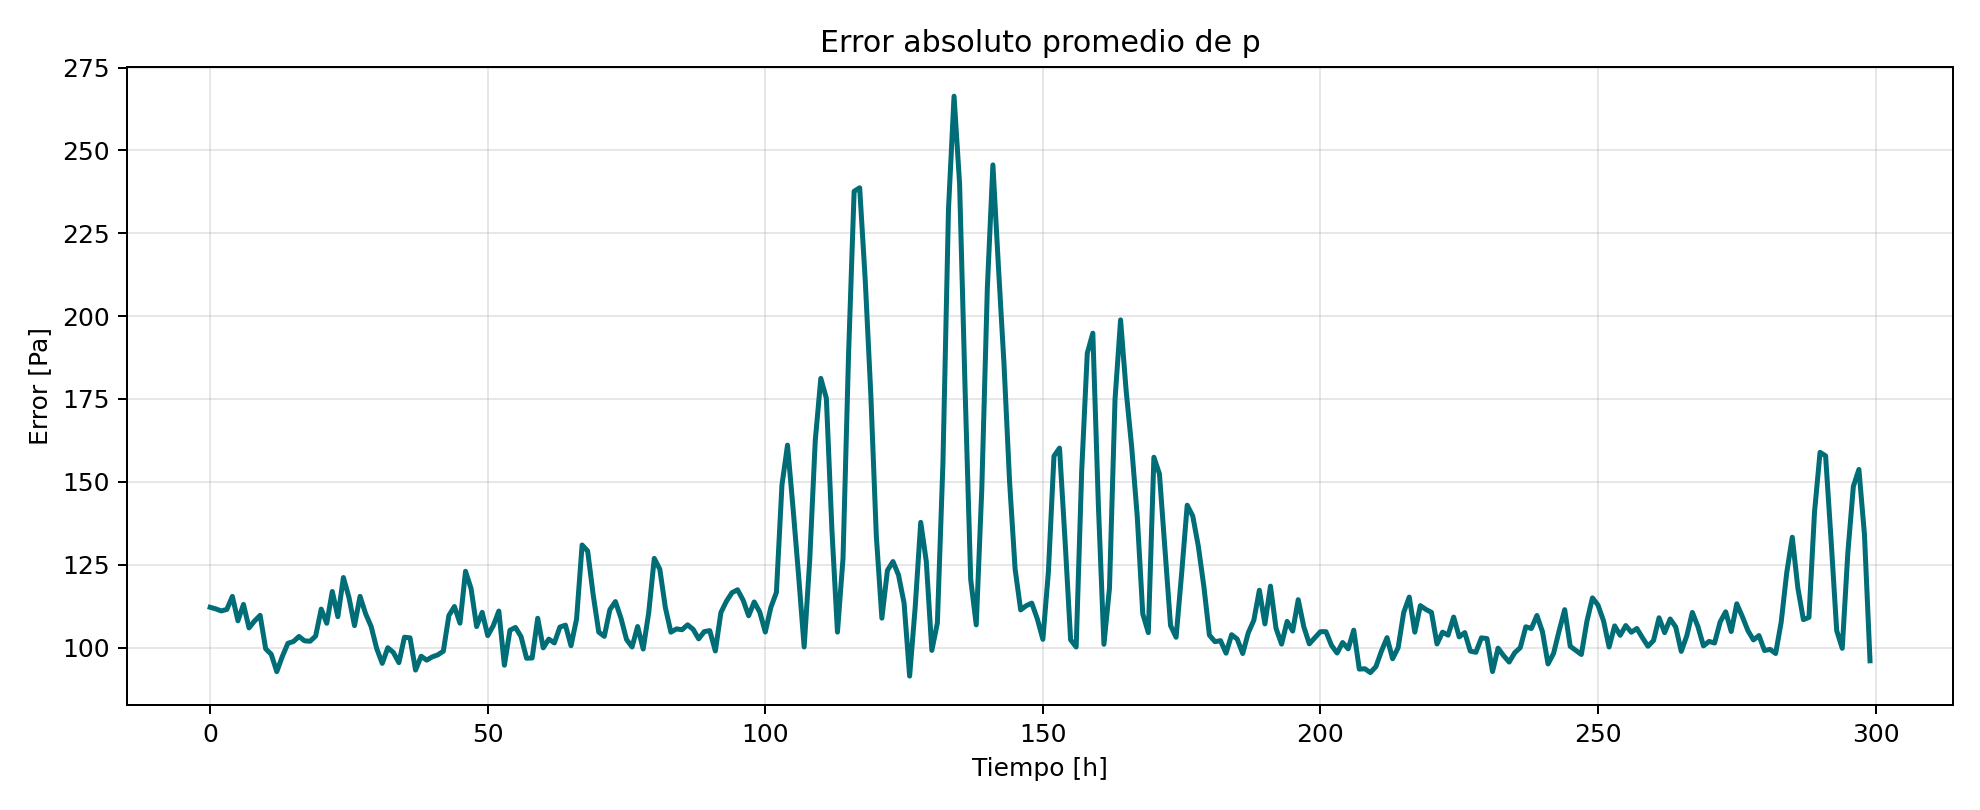
\includegraphics[width=\textwidth]{Imagenes/iter_R01/PINN_caribe_excl4_300xest_R01_L5/pinn_caribe_excl4_300xest_r01_l5_epoca_2000_error_promedio_p_tiempo.png}
  \caption{Error absoluto promedio de la presion $p$ en Pa.}
\end{subfigure}
\caption{Error absoluto promedio en funcion del tiempo para la corrida \texttt{R01\_L5} ($R=0{,}1^\circ$, $\lambda=5$), epoca 2000.}
\label{fig:error_r01_l5}
\end{figure}

\begin{figure}[H]
\centering
\begin{subfigure}[b]{0.85\textwidth}
  \centering
  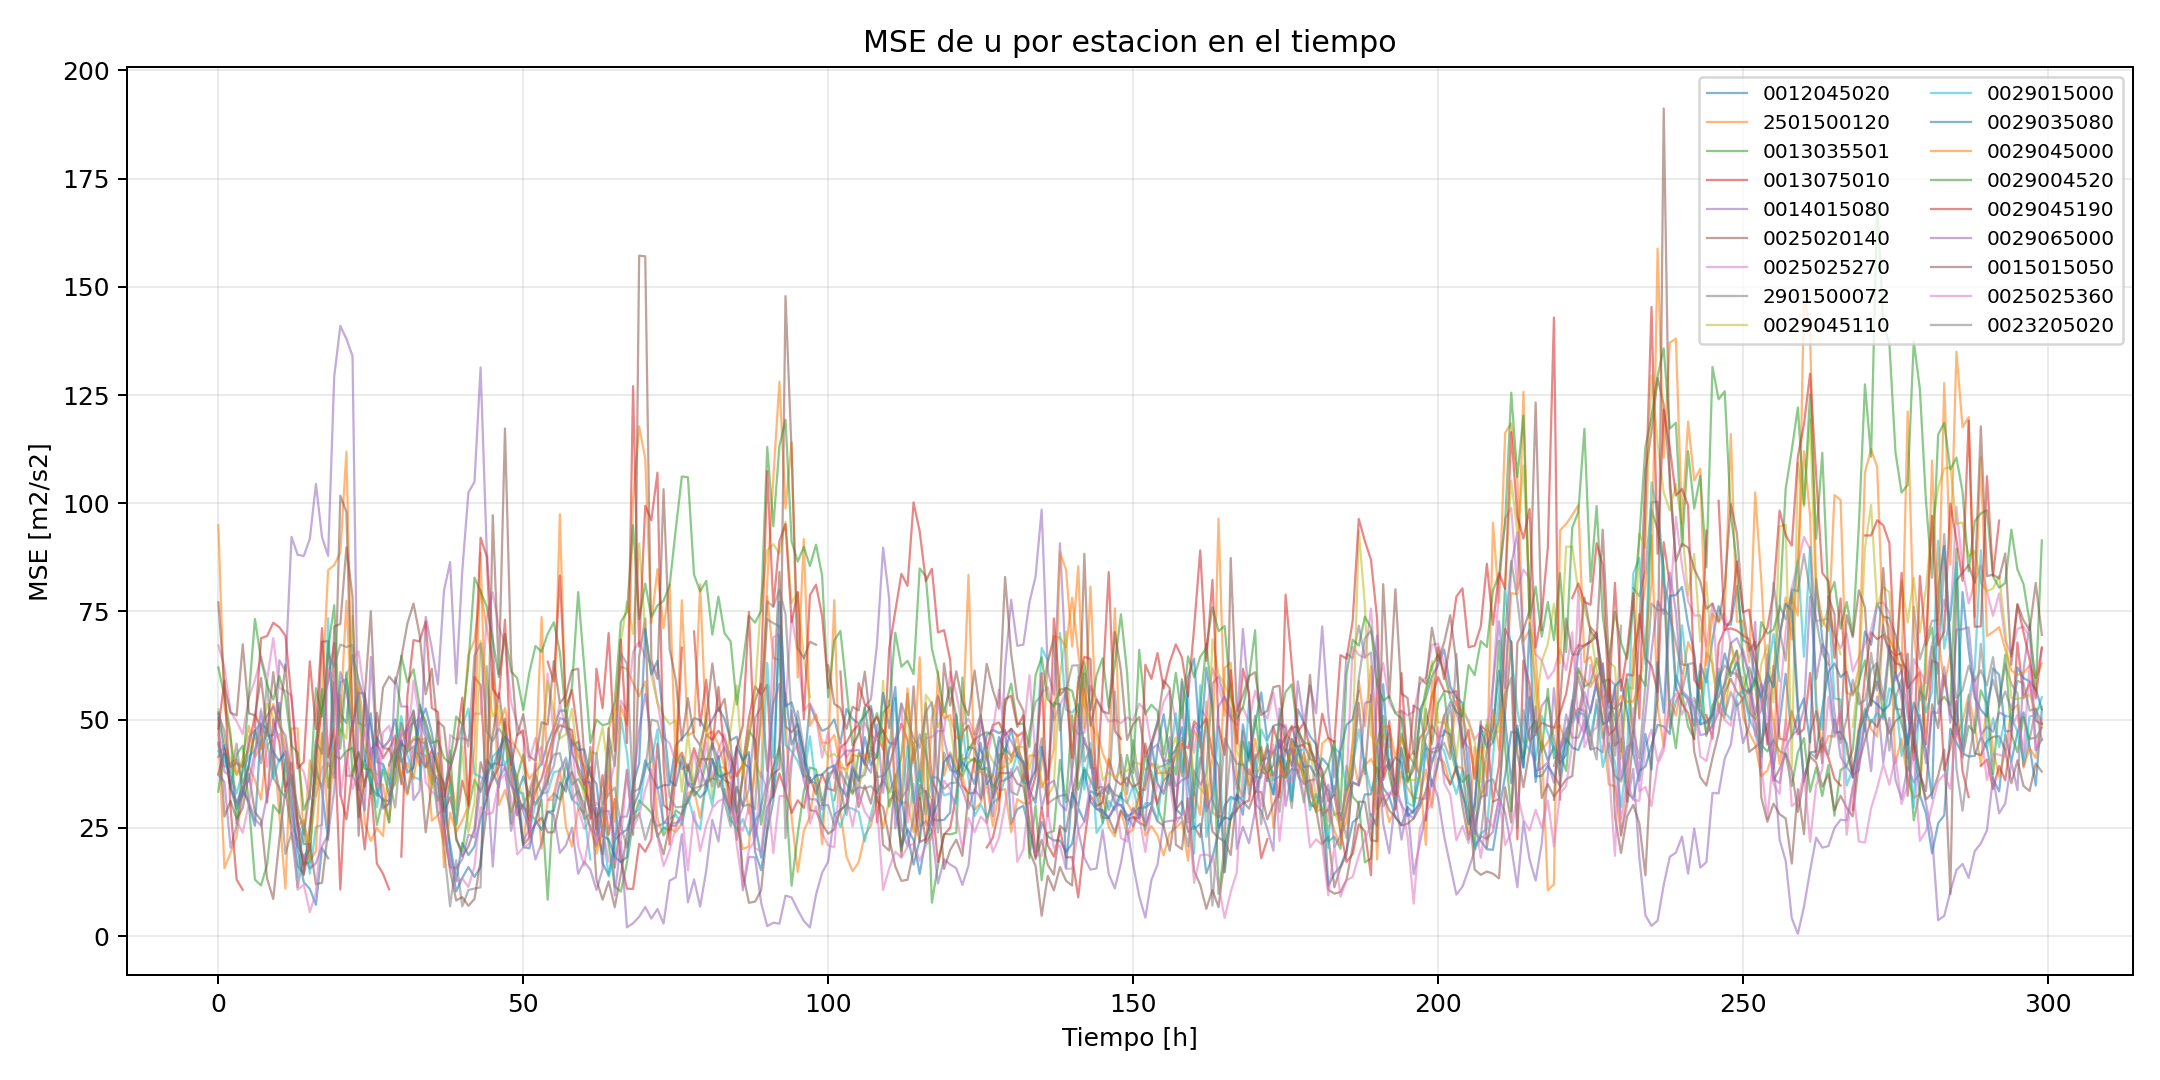
\includegraphics[width=\textwidth]{Imagenes/iter_R01/PINN_caribe_excl4_300xest_R01_L5/pinn_caribe_excl4_300xest_r01_l5_epoca_2000_mse_por_estacion_u_tiempo.png}
  \caption{MSE de la componente $u$ por estacion en m$^2$/s$^2$.}
\end{subfigure}
\par\medskip
\begin{subfigure}[b]{0.85\textwidth}
  \centering
  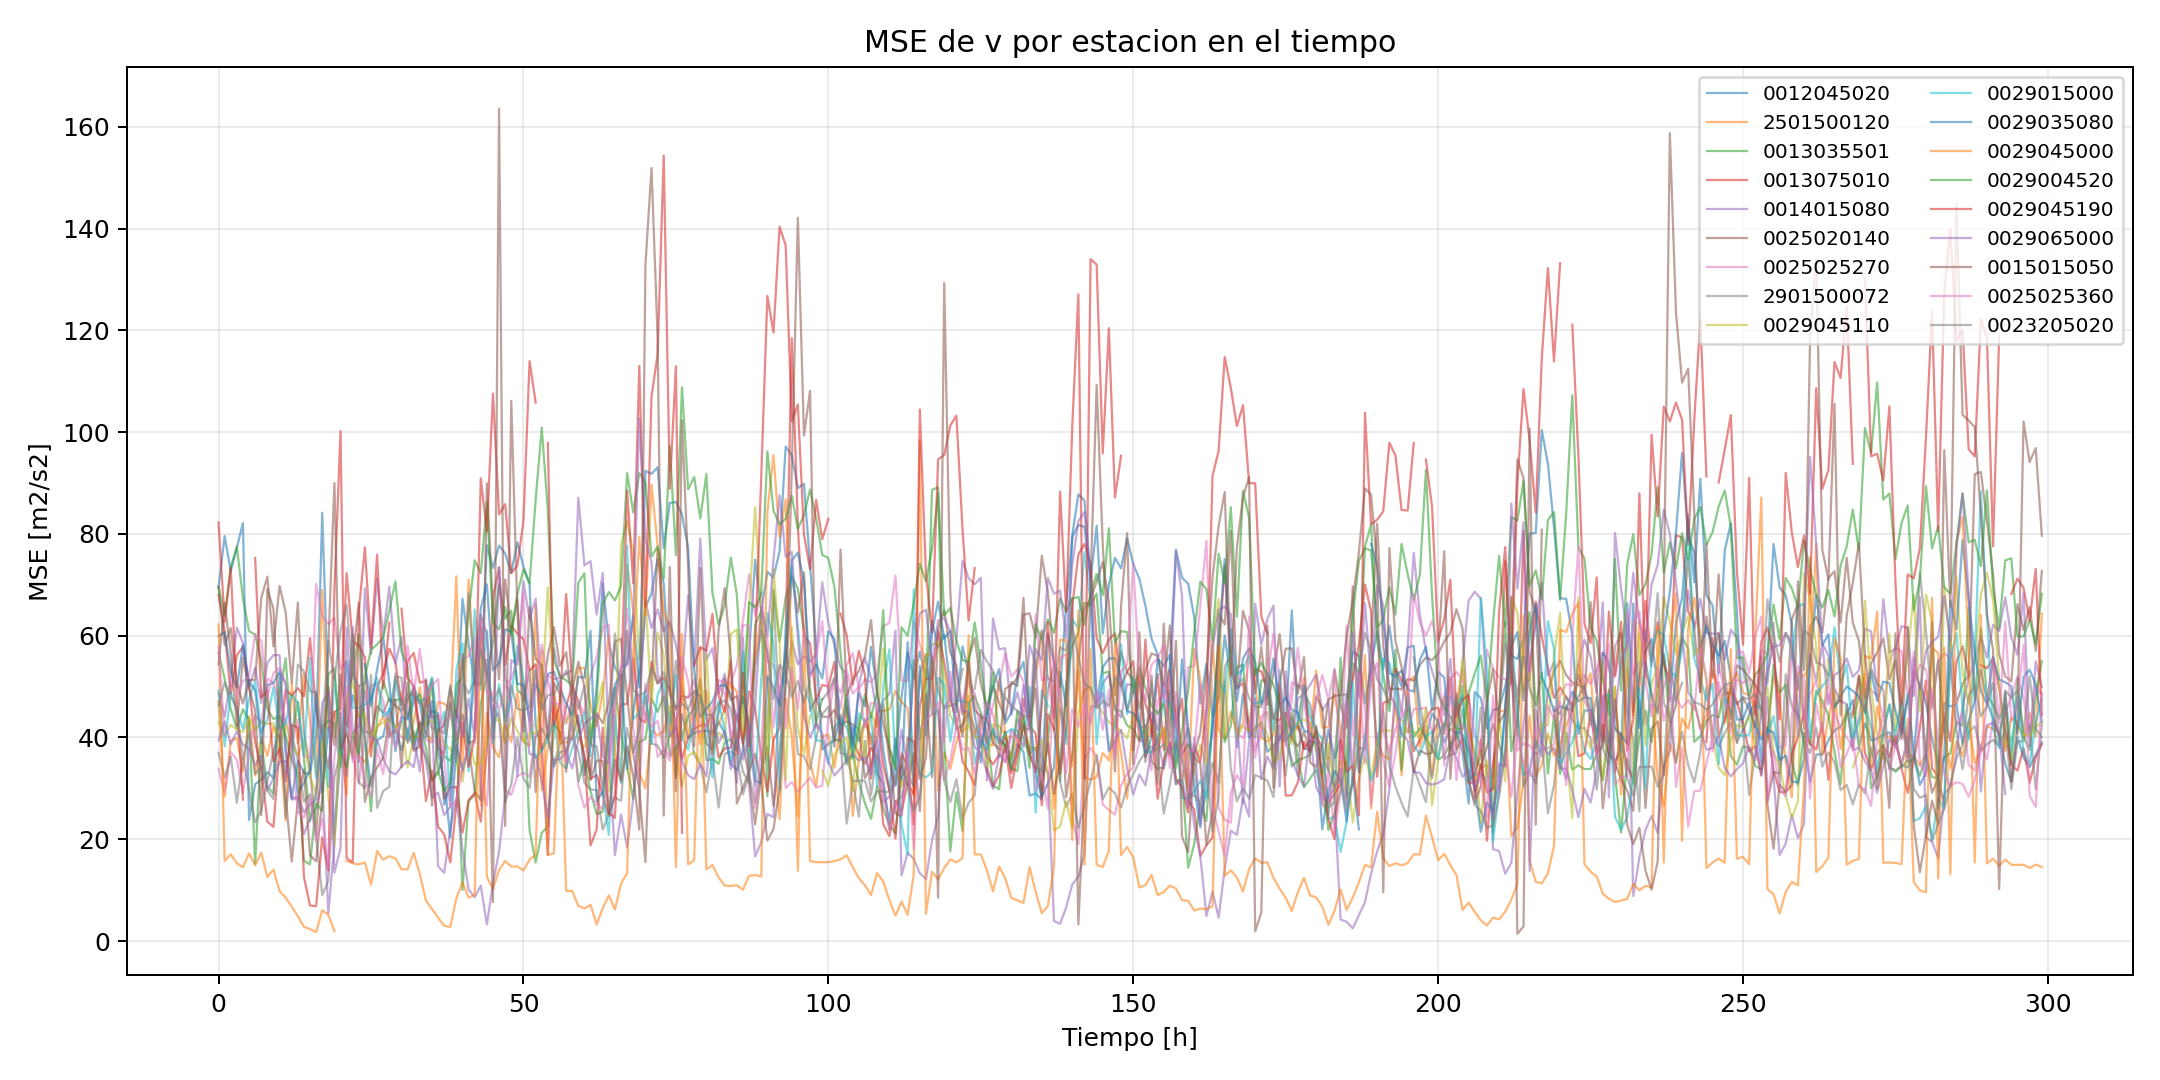
\includegraphics[width=\textwidth]{Imagenes/iter_R01/PINN_caribe_excl4_300xest_R01_L5/pinn_caribe_excl4_300xest_r01_l5_epoca_2000_mse_por_estacion_v_tiempo.png}
  \caption{MSE de la componente $v$ por estacion en m$^2$/s$^2$.}
\end{subfigure}
\par\medskip
\begin{subfigure}[b]{0.85\textwidth}
  \centering
  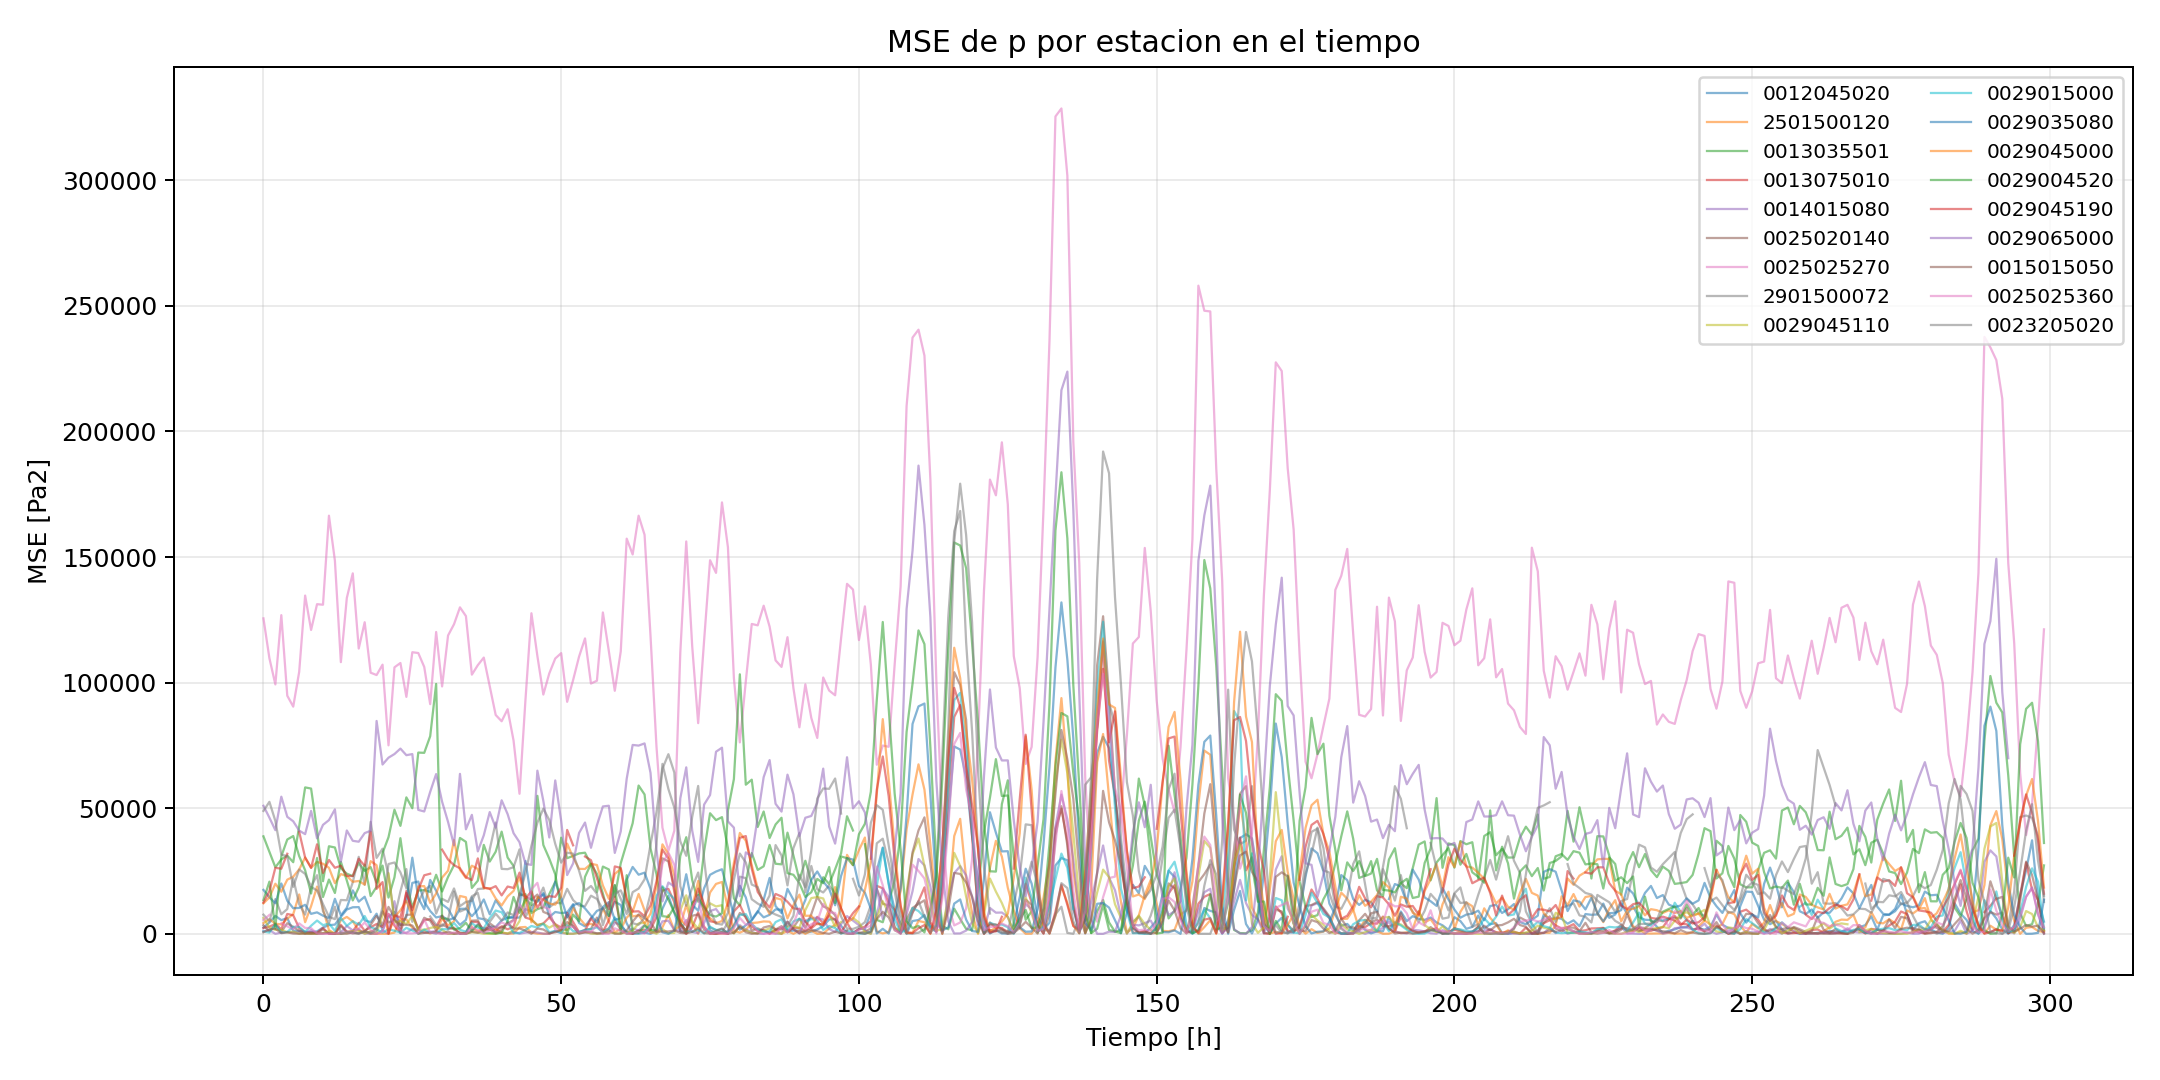
\includegraphics[width=\textwidth]{Imagenes/iter_R01/PINN_caribe_excl4_300xest_R01_L5/pinn_caribe_excl4_300xest_r01_l5_epoca_2000_mse_por_estacion_p_tiempo.png}
  \caption{MSE de la presion $p$ por estacion en Pa$^2$.}
\end{subfigure}
\caption{MSE por estacion en funcion del tiempo para la corrida \texttt{R01\_L5}, epoca 2000.}
\label{fig:mse_r01_l5}
\end{figure}

Las Figuras~\ref{fig:error_r04_l1} y~\ref{fig:mse_r04_l1} presentan la configuracion \texttt{R04\_L1}, que fue la mejor del bloque $R=0{,}4^\circ$ en criterio observacional.

\begin{figure}[H]
\centering
\begin{subfigure}[b]{0.85\textwidth}
  \centering
  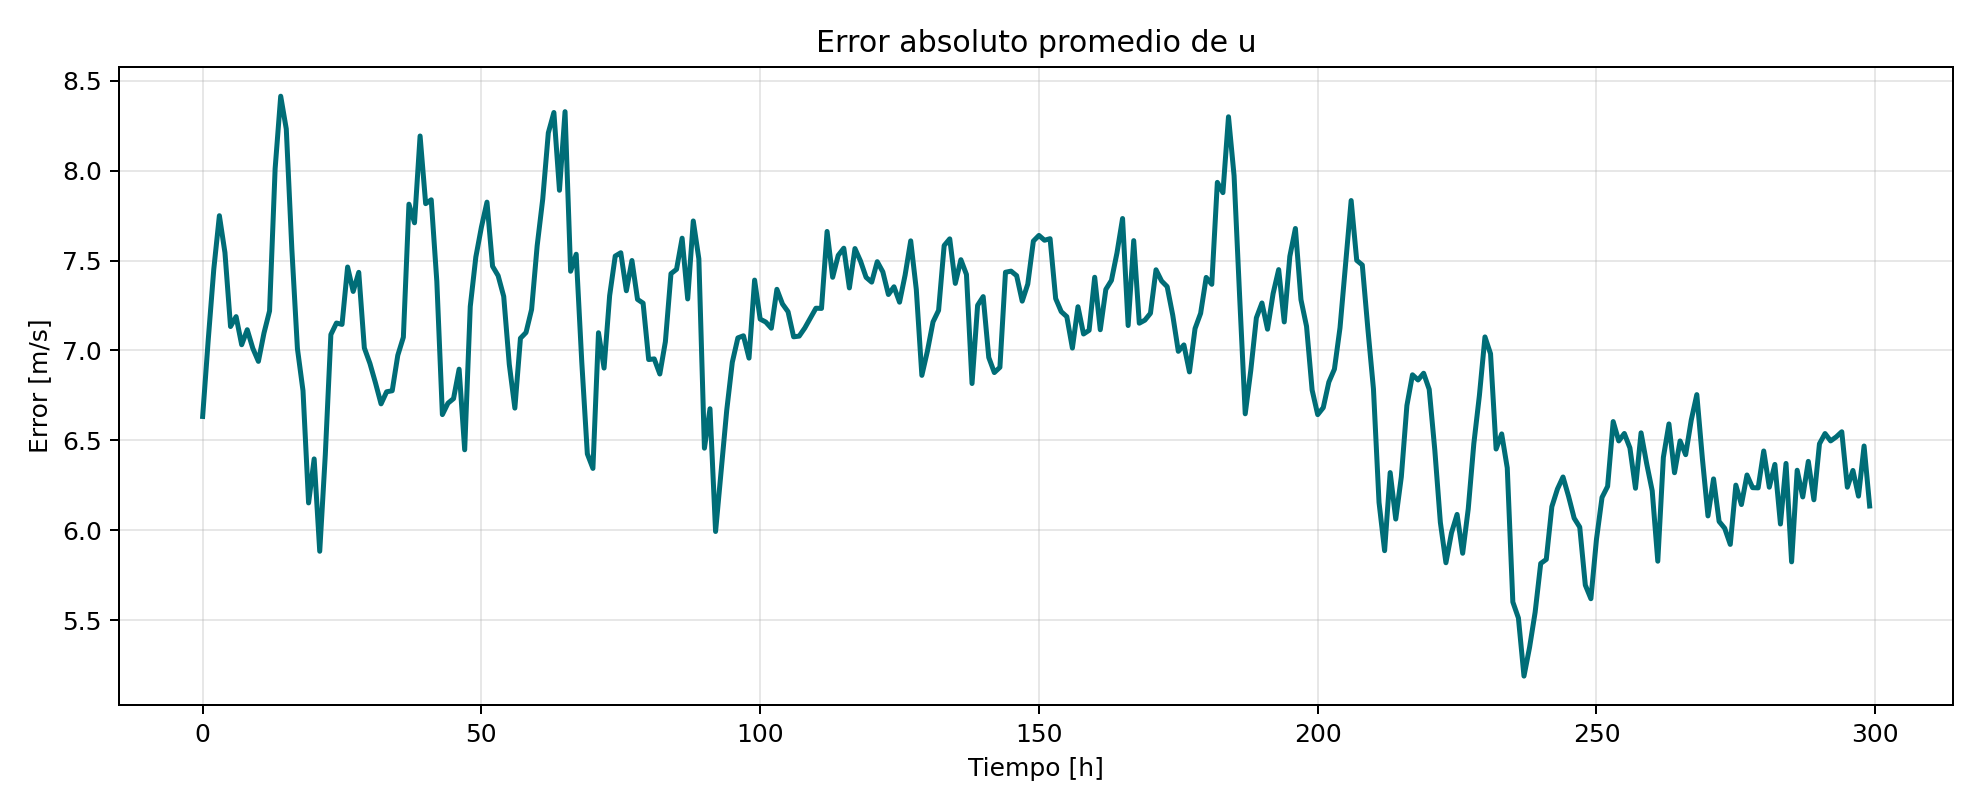
\includegraphics[width=\textwidth]{Imagenes/iter_R04_analisis_20260423/PINN_caribe_excl4_300xest_R04_L1/pinn_caribe_excl4_300xest_r04_l1_epoca_2000_error_promedio_u_tiempo.png}
  \caption{Error absoluto promedio de la componente $u$ (Este--Oeste) en m/s.}
\end{subfigure}
\par\medskip
\begin{subfigure}[b]{0.85\textwidth}
  \centering
  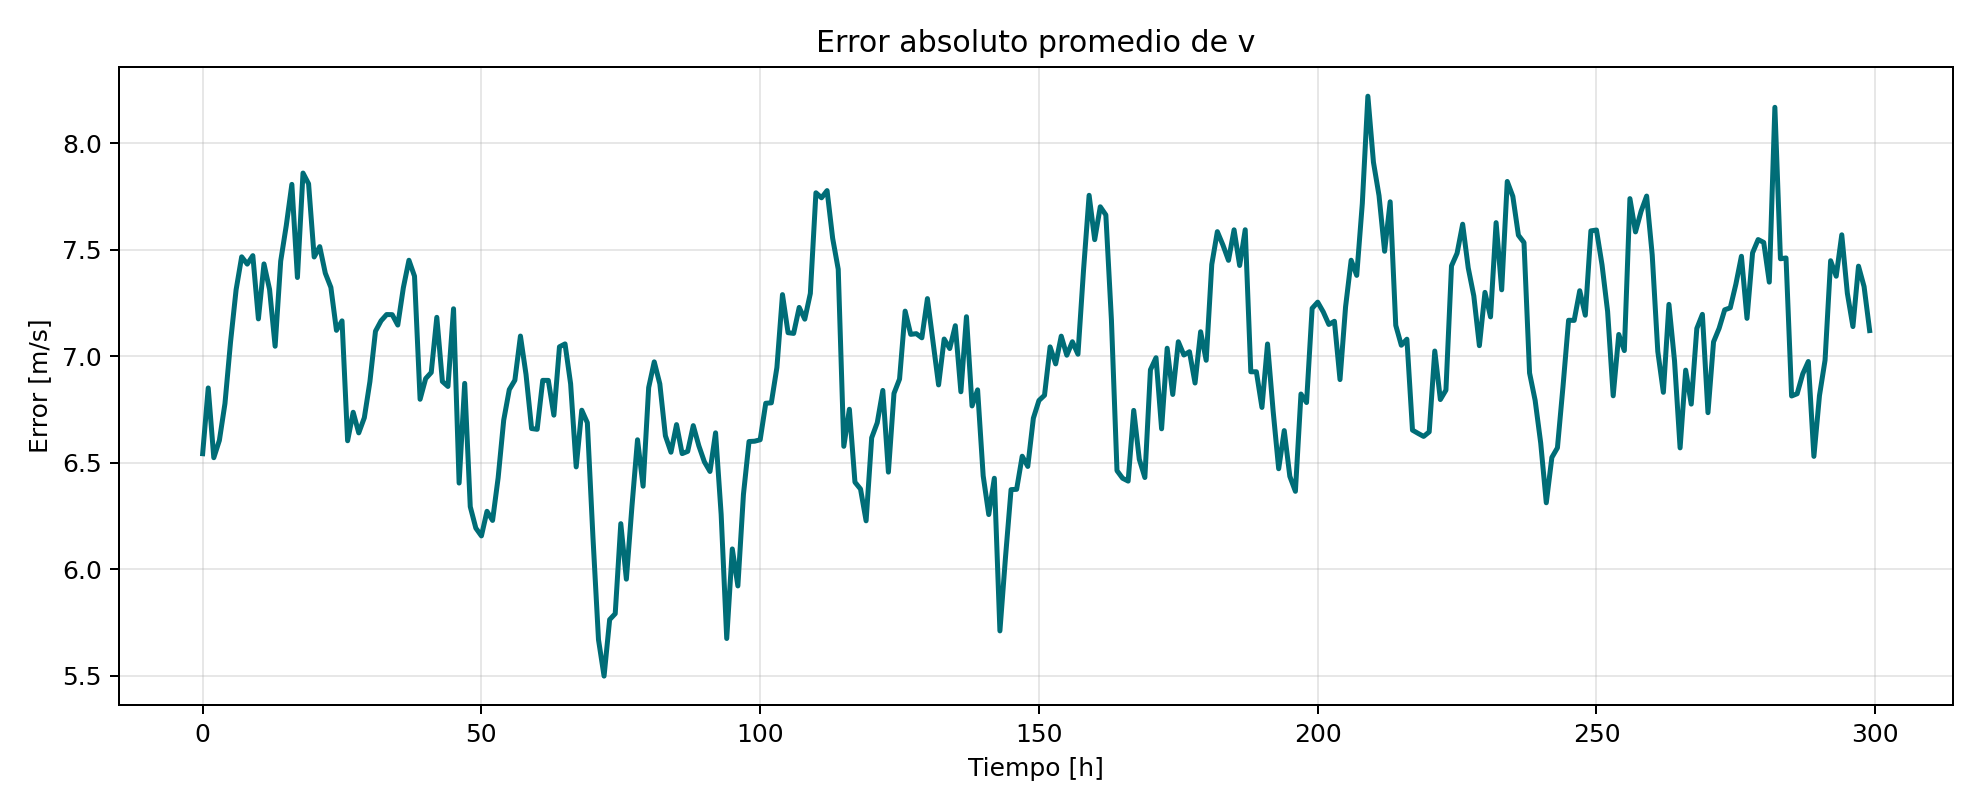
\includegraphics[width=\textwidth]{Imagenes/iter_R04_analisis_20260423/PINN_caribe_excl4_300xest_R04_L1/pinn_caribe_excl4_300xest_r04_l1_epoca_2000_error_promedio_v_tiempo.png}
  \caption{Error absoluto promedio de la componente $v$ (Norte--Sur) en m/s.}
\end{subfigure}
\par\medskip
\begin{subfigure}[b]{0.85\textwidth}
  \centering
  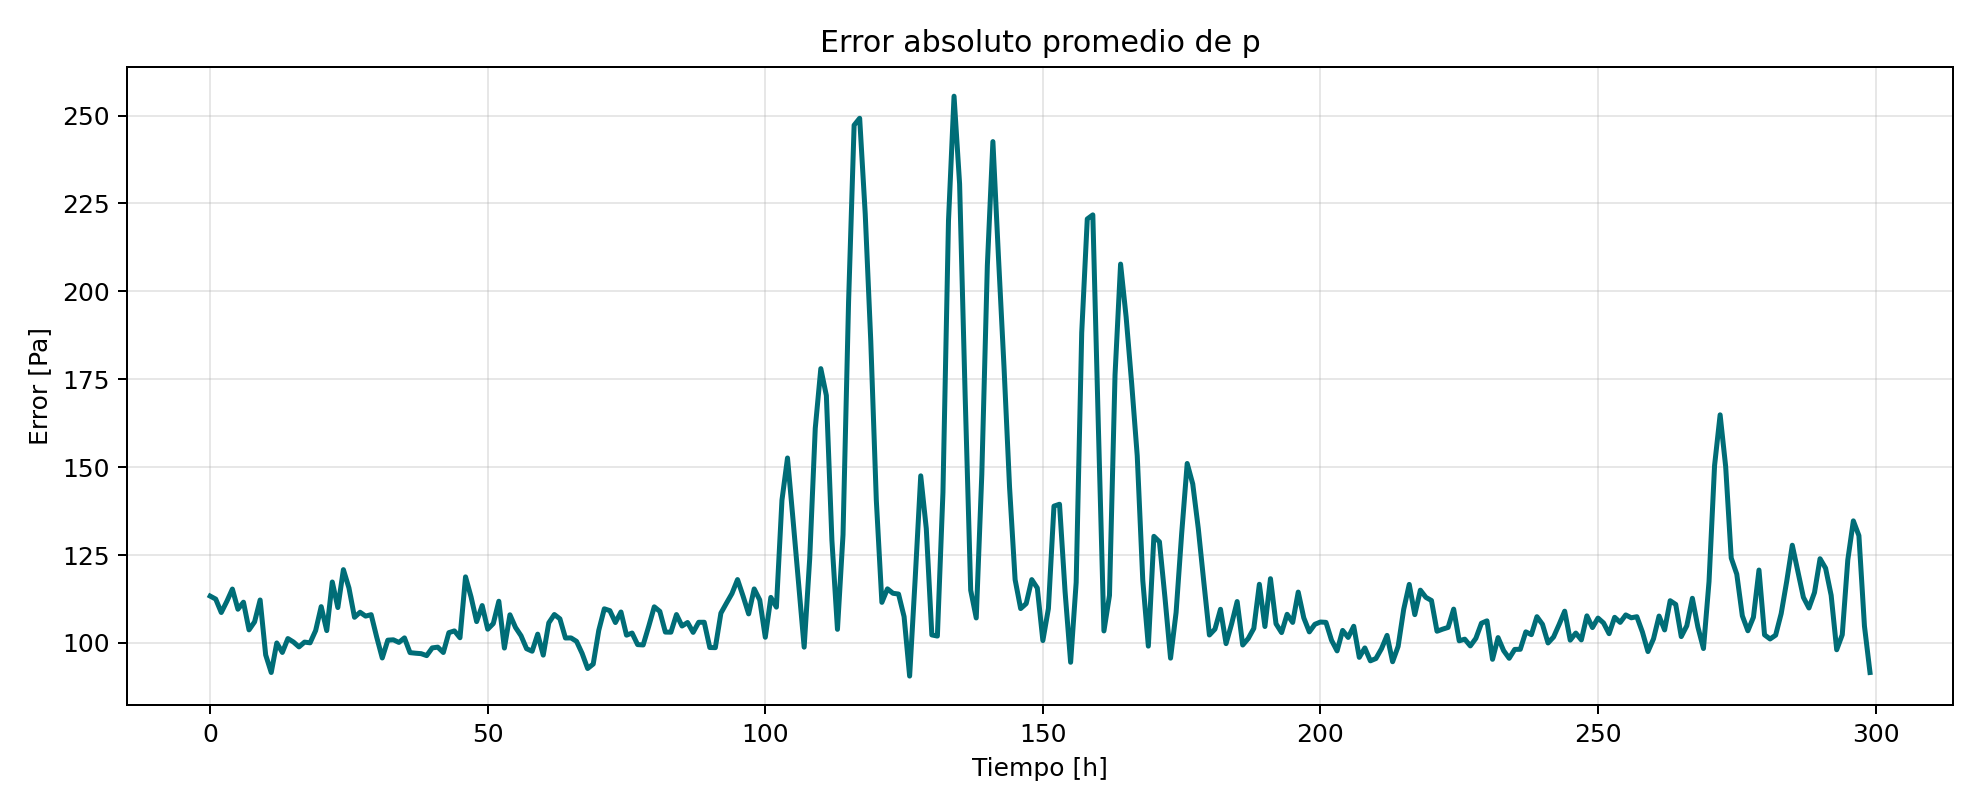
\includegraphics[width=\textwidth]{Imagenes/iter_R04_analisis_20260423/PINN_caribe_excl4_300xest_R04_L1/pinn_caribe_excl4_300xest_r04_l1_epoca_2000_error_promedio_p_tiempo.png}
  \caption{Error absoluto promedio de la presion $p$ en Pa.}
\end{subfigure}
\caption{Error absoluto promedio en funcion del tiempo para \texttt{R04\_L1} ($R=0{,}4^\circ$, $\lambda=1$), epoca 2000.}
\label{fig:error_r04_l1}
\end{figure}

\begin{figure}[H]
\centering
\begin{subfigure}[b]{0.85\textwidth}
  \centering
  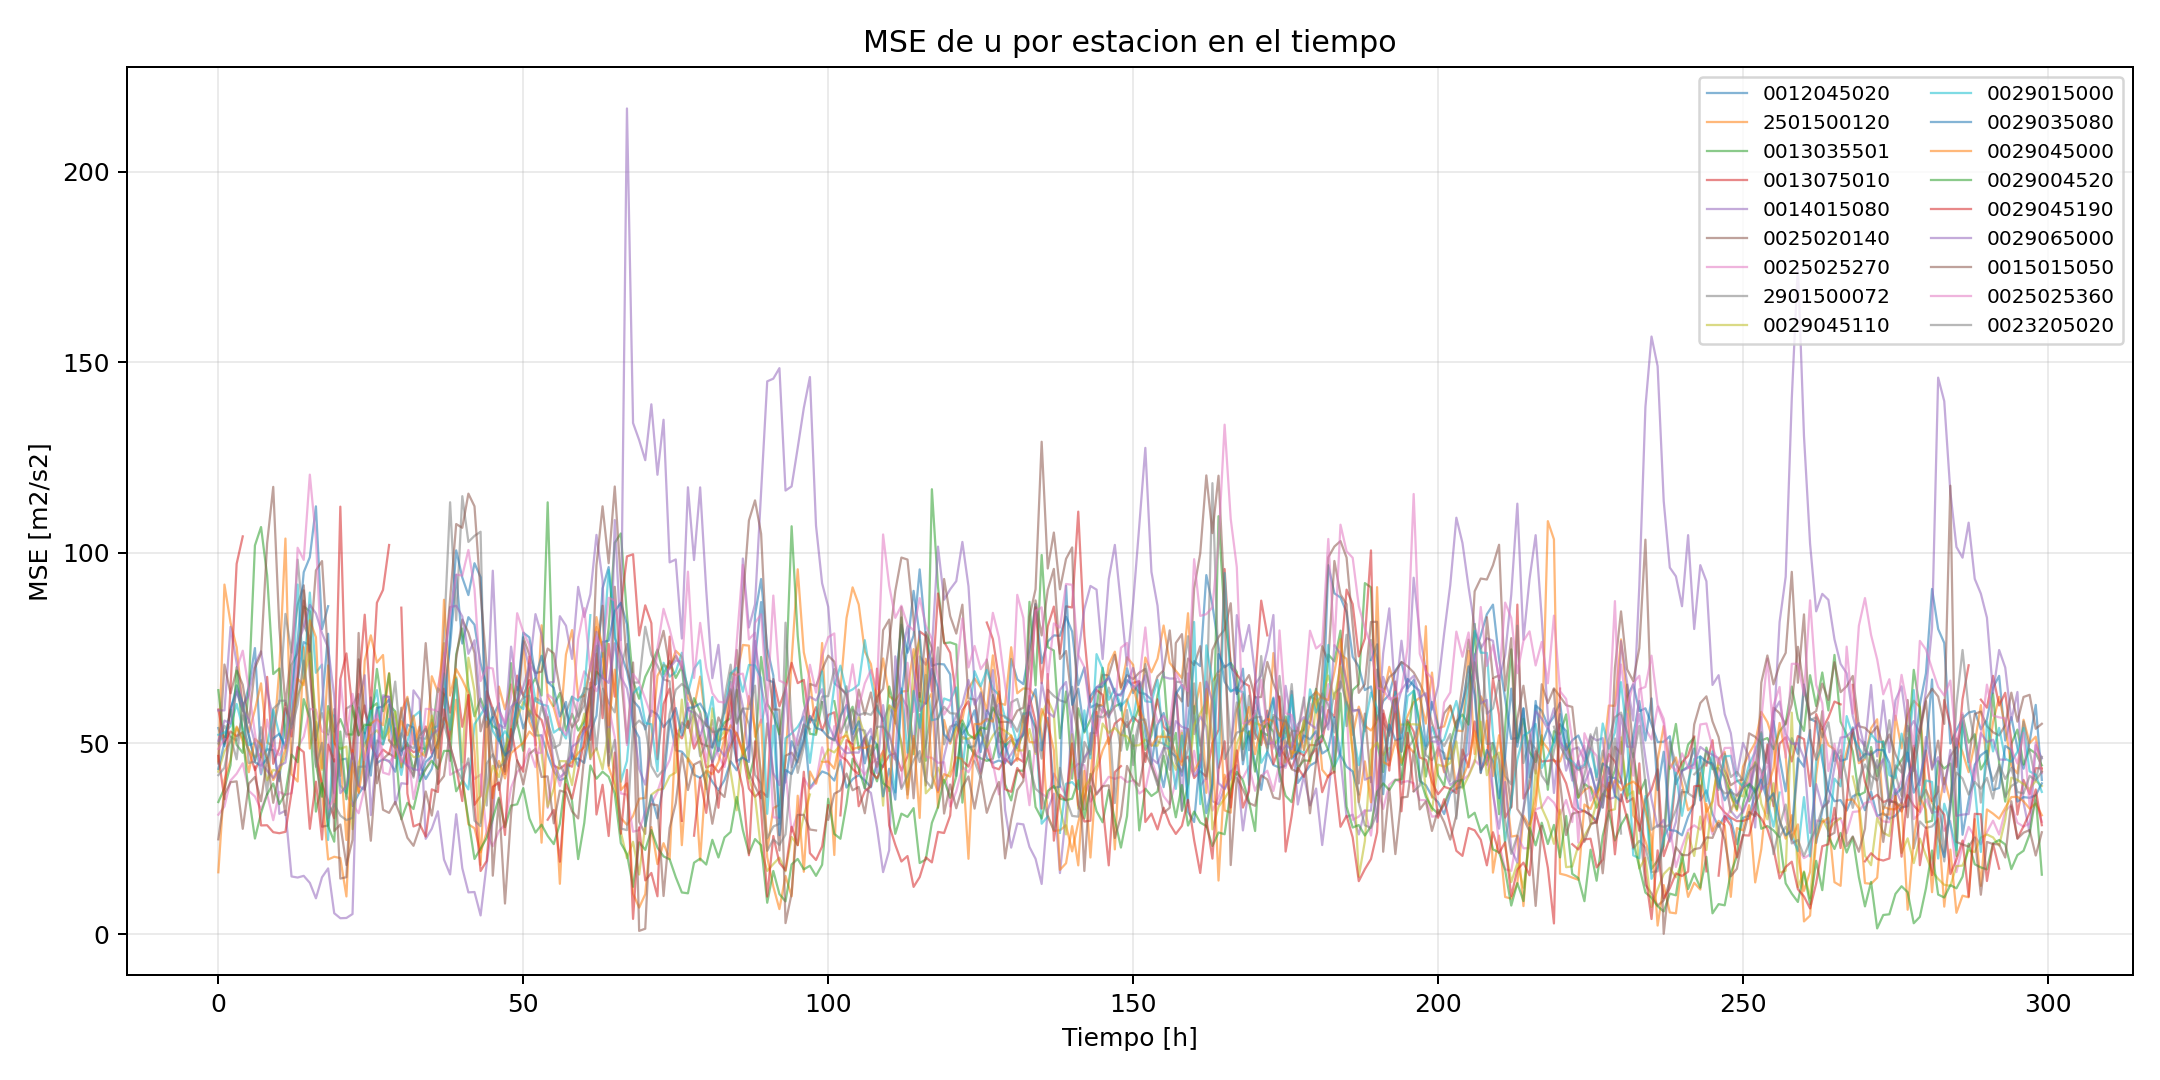
\includegraphics[width=\textwidth]{Imagenes/iter_R04_analisis_20260423/PINN_caribe_excl4_300xest_R04_L1/pinn_caribe_excl4_300xest_r04_l1_epoca_2000_mse_por_estacion_u_tiempo.png}
  \caption{MSE de la componente $u$ por estacion en m$^2$/s$^2$.}
\end{subfigure}
\par\medskip
\begin{subfigure}[b]{0.85\textwidth}
  \centering
  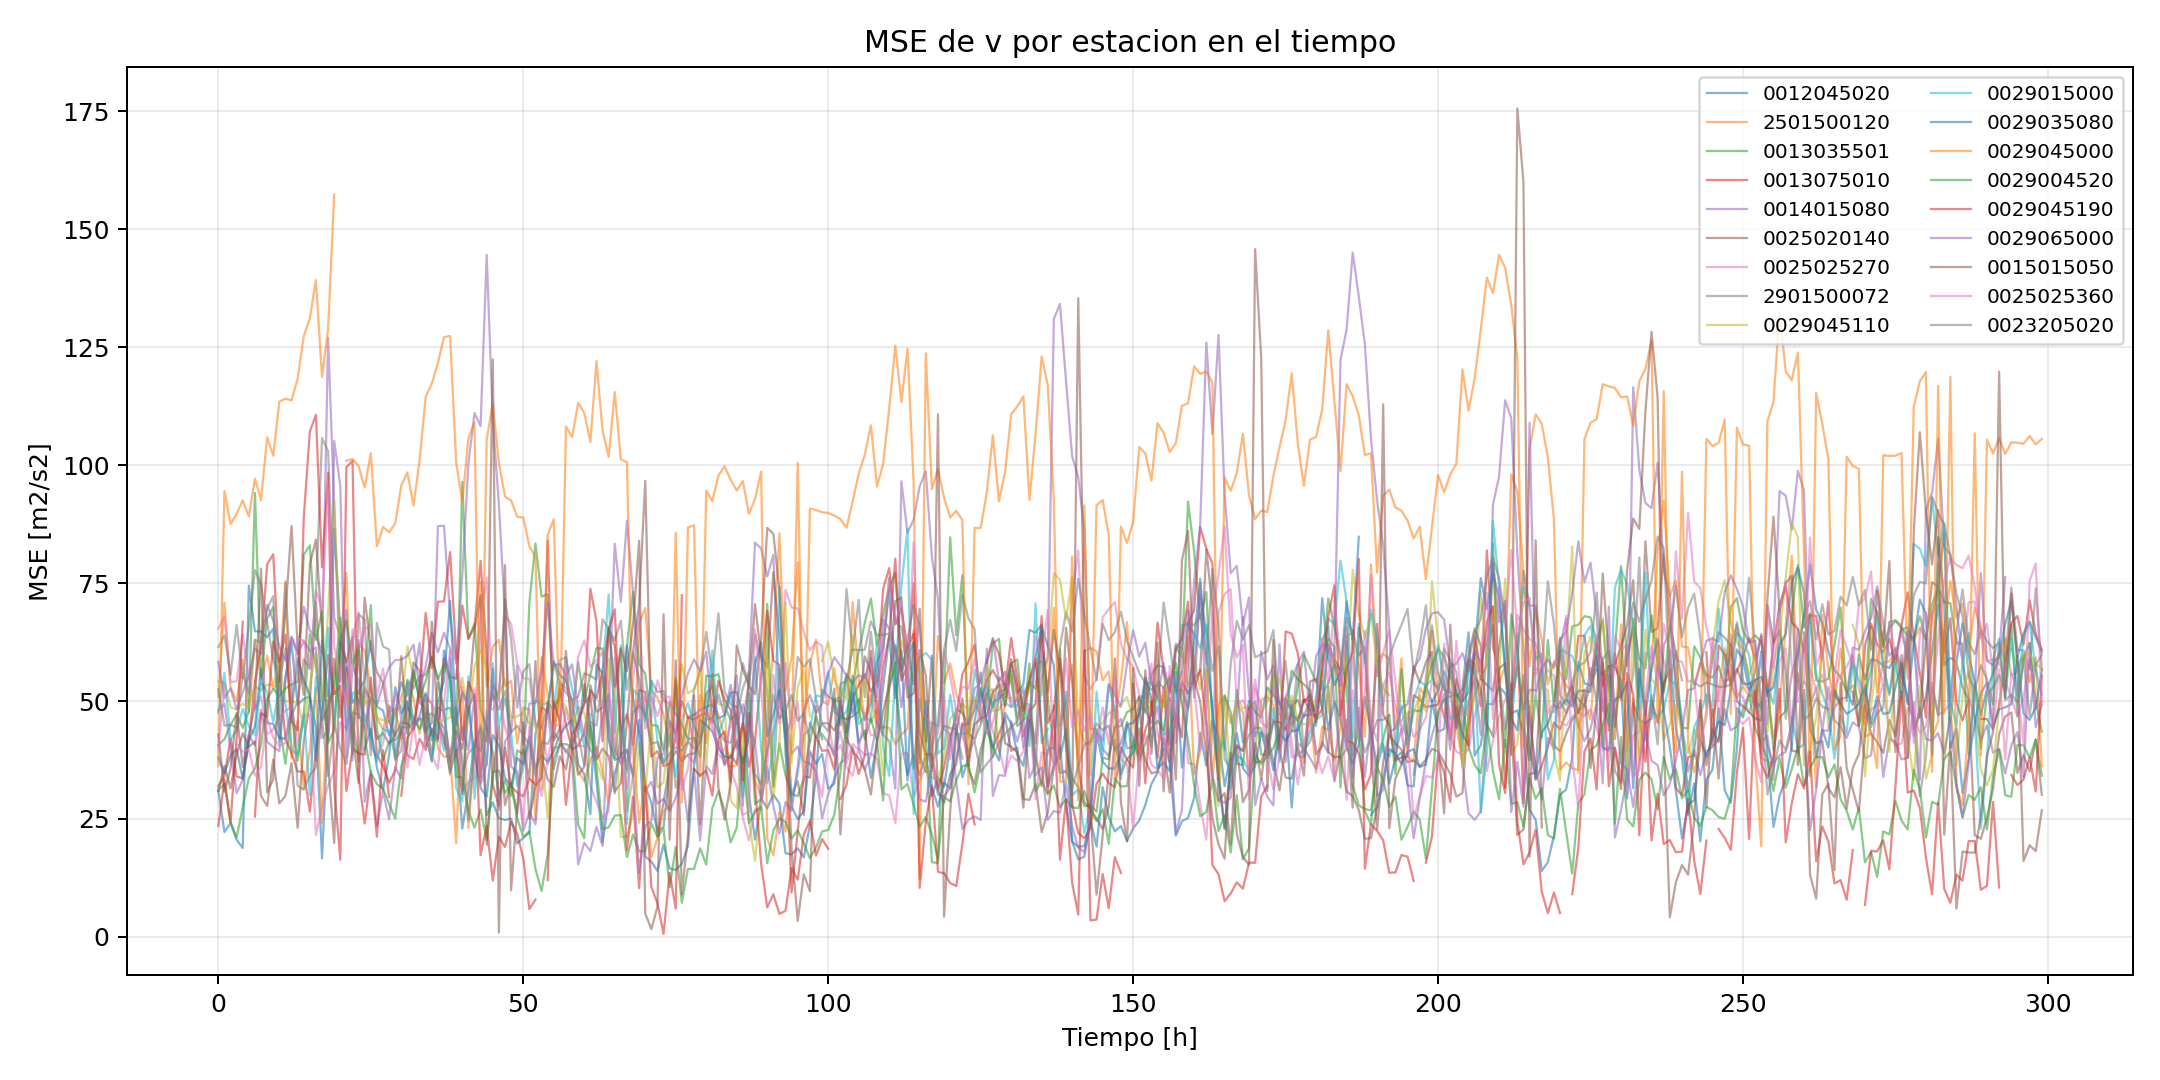
\includegraphics[width=\textwidth]{Imagenes/iter_R04_analisis_20260423/PINN_caribe_excl4_300xest_R04_L1/pinn_caribe_excl4_300xest_r04_l1_epoca_2000_mse_por_estacion_v_tiempo.png}
  \caption{MSE de la componente $v$ por estacion en m$^2$/s$^2$.}
\end{subfigure}
\par\medskip
\begin{subfigure}[b]{0.85\textwidth}
  \centering
  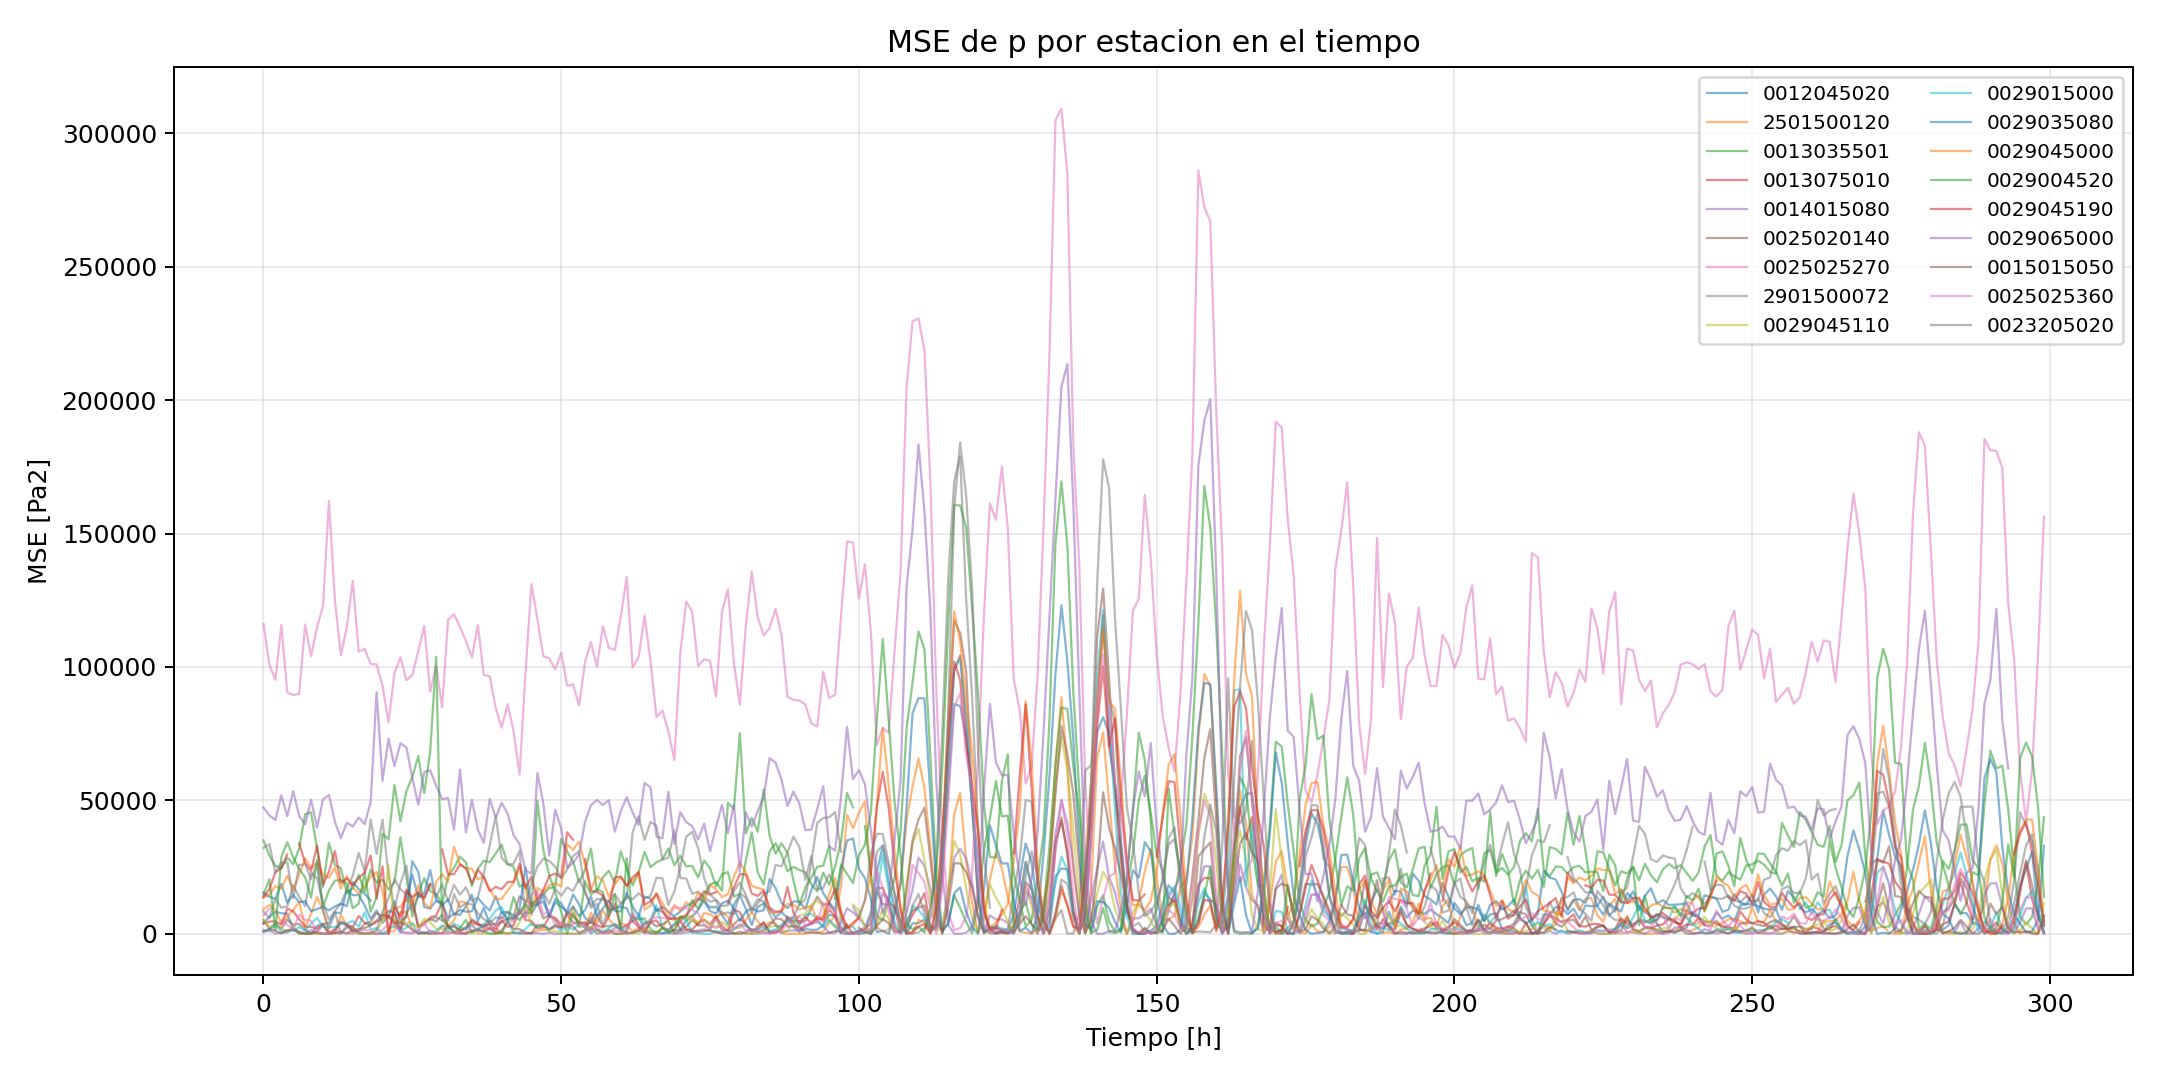
\includegraphics[width=\textwidth]{Imagenes/iter_R04_analisis_20260423/PINN_caribe_excl4_300xest_R04_L1/pinn_caribe_excl4_300xest_r04_l1_epoca_2000_mse_por_estacion_p_tiempo.png}
  \caption{MSE de la presion $p$ por estacion en Pa$^2$.}
\end{subfigure}
\caption{MSE por estacion en funcion del tiempo para \texttt{R04\_L1}, epoca 2000.}
\label{fig:mse_r04_l1}
\end{figure}

\clearpage
\chapter{Discusión}

El consolidado experimental permite discutir hallazgos principales sobre el comportamiento de la PINN en el dominio meteorológico Caribe y sobre el papel de la física como regularizador en redes neuronales.

La evidencia descriptiva presentada en la Figura~\ref{fig:serie_temporal_datos_caribe} y la Figura~\ref{fig:hist_temp_caribe} aporta contexto para esta discusion: el conjunto exhibe variabilidad temporal apreciable y una distribucion termica concentrada en un rango principal con colas menos densas. En conjunto, estas caracteristicas son coherentes con la necesidad de balancear ajuste observacional y regularizacion fisica durante el entrenamiento, en lugar de optimizar solo uno de los dos objetivos.

\section{Naturaleza del trade-off observacional-físico}

Los resultados confirman una tensión inherente entre dos objetivos: minimizar el error frente a observaciones y minimizar el residual de Navier-Stokes. Sin embargo, el trade-off no es monolítico.

En el bloque $R=0{,}1^{\circ}$ con 300 registros por estación, $\lambda=5$ logró el mejor equilibrio observacional ($\overline{\text{MSE}}_{\text{obs}}=0{,}85185$) con residual físico modesto ($0{,}03682$). En contraste, $\lambda=10$ redujo el residual a $0{,}02318$ pero incrementó el error observacional a $0{,}89305$. En el bloque $R=0{,}4^{\circ}$, $\lambda=1$ favoreció el ajuste a datos ($0{,}86216$) pero dejó un residual elevado ($0{,}24141$), mientras $\lambda=10$ invirtió la prioridad ($0{,}88765$ en error, $0{,}02242$ en residual).

Este patrón es consistente con la formulación de la función de pérdida combinada $\mathcal{L}_{\text{total}} = \lambda \cdot \mathcal{L}_{\text{NS}}^2 + \mathcal{L}_{u_x}^2 + \mathcal{L}_{u_y}^2 + \mathcal{L}_p^2$. El multiplicador $\lambda$ es un control explícito de preferencia: valores bajos prioriza ajuste a datos, valores altos imponen coherencia física. La pregunta científica es cuál balance es más apropiado para predicción meteorológica; en este proyecto, $\lambda=5$ emerge como un punto de equilibrio práctico.

\section{Patrón crítico: inefectividad de \texorpdfstring{$\lambda = 3$}{lambda = 3}}

Un hallazgo metodológico sorprendente es que $\lambda=3$ produce desempeño consistentemente desfavorable en ambas resoluciones de malla. Comparando valores adyacentes:
\begin{itemize}
	\item En R=0,1°: $\lambda=3$ produce $\overline{\text{MSE}}_{\text{obs}} = 1,24982$, superior tanto a $\lambda=1$ (0,86796) como a $\lambda=5$ (0,85185) y $\lambda=10$ (0,89305).
	\item En R=0,4°: $\lambda=3$ genera $\overline{\text{MSE}}_{\text{obs}} = 1,02208$, inferior a $\lambda=1$ (0,86216) pero superior a $\lambda=5$ (1,32126) y $\lambda=10$ (0,88765).
\end{itemize}

Esto sugiere que el valor específico $\lambda=3$ introduce una tensión desequilibrada entre términos de la función de pérdida, posiblemente porque la magnitud relativa de $\lambda \cdot \mathcal{L}_{\text{NS}}$ respecto a $\mathcal{L}_{\text{datos}}$ en esa malla crea un paisaje de optimización problemático. Futuras investigaciones deberían explorar si este patrón persiste en otras arquitecturas o dominios.

\section{Interacción entre \texorpdfstring{$\lambda$}{lambda} y resolución de malla}

El efecto de refinar la malla (de R=0,4° a R=0,1°) no fue uniforme. Con $\lambda=5$, la malla fina fue netamente superior ($\Delta\overline{\text{MSE}} = -0{,}47$ a favor de R=0,1°). Para $\lambda=1$ y $\lambda=10$, el cambio fue marginal o ligeramente a favor de R=0,4°.

Una interpretación física plausible es que una malla más fina (R=0,1°, 91.200 puntos de colocación frente a 13.200) expande significativamente el espacio donde se evalúa la restricción física. Con $\lambda$ bajo, los puntos adicionales quedan subutilizados; con $\lambda$ alto, la malla fina proporciona suficiente información física para constrair la solución efectivamente. Este acoplamiento entre densidad espacial y peso físico tiene implicaciones prácticas: no basta seleccionar $R$ y $\lambda$ independientemente.

\section{Rol de la dominancia de presión en la pérdida combinada}

En las corridas analizadas del proyecto, la pérdida asociada a presión ($\mathcal{L}_p$) representó aproximadamente entre el 40\% y el 60\% de la pérdida total. Este comportamiento es consistente con una asimetría de escala entre variables de salida, donde la presión tiende a aportar magnitudes de error superiores a las componentes de velocidad.

Esta dominancia puede influir en la dinámica de optimización, al aumentar el peso efectivo de la presión dentro del objetivo global y condicionar el equilibrio entre ajuste observacional y restricción física. En consecuencia, parte del comportamiento observado en el barrido de hiperparámetros puede interpretarse como resultado de la interacción entre $\lambda$, resolución de malla y desbalance relativo entre componentes de pérdida.

Como línea de trabajo futuro, se recomienda evaluar estrategias de balanceo entre variables que permitan mantener comparabilidad de magnitudes en la función objetivo, sin alterar la trazabilidad de los experimentos ya reportados.

\section{Efecto regularizador de la restriccion suave de rango}

La incorporacion de una restriccion suave de rango agrega un tercer mecanismo de control al entrenamiento, complementario al ajuste observacional y al residual fisico de Navier-Stokes. Mientras el hiperparametro $\lambda$ regula explicitamente la importancia del termino fisico, la penalizacion de rango opera sobre la plausibilidad de las magnitudes predichas en todo el dominio de colocacion.

La evidencia experimental muestra que, dentro de la configuracion $R=0{,}1^{\circ}$ y $\lambda=5$, la corrida \texttt{todosreg\_R01\_L5\_rangeL05} alcanzo una perdida final de 0,638, inferior a la obtenida por la corrida equivalente sin restriccion de rango y con la totalidad de los registros disponibles (0,926 en \texttt{todos\_R01\_L5}). En la comparacion reportada, este comportamiento es consistente con la hipotesis de que la restriccion suave de rango estabiliza la optimizacion y favorece soluciones mas coherentes con el dominio fisico observado.

La metrica FOR sugiere, ademas, que el efecto del mecanismo no es uniforme entre variables. Al cierre del entrenamiento, la presion mantiene una fraccion fuera de rango practicamente nula, mientras las componentes de velocidad conservan porcentajes mayores. Esto indica que la restriccion de rango no impone un encapsulamiento artificial de toda la solucion, sino una regularizacion diferenciada segun la variable y la region del dominio.

\section{Beneficio sin equivalente arquitectónico: volumen de datos}

La comparación más contundente del proyecto es la mejora al incluir más datos, manteniendo exactamente la arquitectura y configuración. La ampliación de 5.400 a 13.392 registros produjo reducciones simultáneas del 11,3\% en error observacional promedio y del 65,4\% en residual físico. Esto demuestra que:

\begin{enumerate}
	\item El modelo PINN en esta configuración aún opera en régimen de datos limitados (no ha saturado).
	\item La cobertura temporal en diciembre de 2025 no es suficientemente redundante; los 744 registros por estación aportan información genuina.
	\item La restricción física de Navier-Stokes se vuelve más efectiva cuando hay más datos que la justifiquen.
\end{enumerate}

Este resultado tiene implicaciones prácticas: si el objetivo es mejorar el modelo actual, la estrategia más clara es ampliar la cobertura temporal, antes que buscar arquitecturas alternativas.

\section{Alcance y limitaciones del análisis}

La evaluación de generalización temporal realizada mediante partición de los datos en
entrenamiento (días 1–20) y prueba independiente (días 21–31) revela un patrón mixto que
matiza el alcance de los resultados. Las componentes de velocidad del viento muestran
degradación inferior al $5$\,\% en el conjunto de prueba ($\text{MSE}_{u_x}$: $-4{,}5$\,\%;
$\text{MSE}_{u_y}$: $-2{,}3$\,\%), lo que indica que la restricción física de Navier-Stokes
actúa como regularizador eficaz y favorece la transferencia temporal del campo de viento.
En contraste, el $\text{MSE}$ de presión se incrementa un $185{,}8$\,\% en el período de prueba
($1{,}3688 \to 3{,}9116$), confirmando sobreajuste en esta variable fuera del intervalo de
entrenamiento. El residual de Navier-Stokes también aumenta de forma proporcional
($0{,}01273 \to 0{,}03640$, $+186{,}0$\,\%), indicando que la coherencia física aprendida en
los primeros 20 días no se transfiere plenamente a los 11 días siguientes.

Este patrón asimétrico es consistente con las diferencias de variabilidad temporal entre
variables: la presión atmosférica tiende a presentar mayores fluctuaciones de período
medio-largo que las componentes de viento, lo que la hace más sensible a la extensión del
período de entrenamiento. La restricción física de Navier-Stokes, al ser una ecuación
cinemática local, regula la suavidad espacial del campo de velocidades con mayor eficacia
que la evolución temporal de la presión.

En consecuencia, las predicciones de viento del modelo pueden considerarse razonablemente
confiables dentro del dominio y período estudiados, mientras que las predicciones de presión
deben interpretarse con cautela fuera del período de entrenamiento. Además, el bloque
$R=0{,}2^{\circ}$ permanece incompleto para varios valores de $\lambda$, por lo que el ranking
final se interpreta sobre las corridas efectivamente evaluadas en su totalidad.



\clearpage
\chapter{Conclusiones}

\section{Sintesis integrada}

Esta propuesta de cierre condensa los resultados del estudio en una lectura unificada y no fragmentada. La evidencia obtenida confirma que una PINN con restriccion fisica basada en Navier-Stokes inviscido puede capturar patrones meteorologicos relevantes del Caribe colombiano con datos observacionales dispersos, siempre que el balance entre ajuste a datos y regularizacion fisica se mantenga en una zona intermedia. En ese marco, la configuracion \nolinkurl{PINN_caribe_excl4_todos_R01_L5} se consolida como la referencia mas consistente del trabajo, al combinar el menor error observacional promedio reportado con el residual fisico mas bajo entre las corridas comparables.

Tambien se observa que el desempeno no depende de un unico hiperparametro aislado, sino de la interaccion entre peso fisico, resolucion de malla y volumen de datos. La mejora al pasar de 5.400 a 13.392 registros, sin cambios de arquitectura, sugiere que el regimen experimental todavia estaba condicionado por disponibilidad de datos. De forma complementaria, la restriccion suave de rango mostro un efecto favorable sobre el ajuste observacional y la perdida total en la configuracion evaluada, aunque con un aumento moderado del residual fisico, lo que indica que su aporte es prometedor pero aun requiere ajuste para lograr un compromiso mas estable.

\section{Alcance y proyeccion del estudio}

El alcance de estas conclusiones debe leerse con cautela metodologica. Aunque la aproximacion demuestra viabilidad tecnica y consistencia interna en el dominio analizado, la generalizacion fuera del periodo de entrenamiento es parcial: el comportamiento del viento se mantiene razonablemente estable, mientras que la presion presenta deterioro apreciable en prueba temporal independiente. A esto se suma que el barrido no cubre por completo todos los escenarios previstos, que la validacion comparativa con metodos de referencia no se incluyo en esta etapa y que la formulacion fisica omite el termino de Coriolis, aun cuando el numero de Rossby estimado para el dominio sugiere una influencia no despreciable de la rotacion terrestre.

En consecuencia, la contribucion principal de este trabajo es establecer una linea base solida, trazable y tecnicamente defendible para la modelacion PINN en el Caribe colombiano, junto con una ruta clara de continuidad: completar el espacio experimental pendiente, reforzar la validacion fuera de muestra e incorporar extensiones fisicas y comparativas que permitan evaluar robustez y transferibilidad del modelo mas alla del periodo estudiado.






\clearpage

% ====== Bibliografía ======
\clearpage
\bibliographystyle{apacite}
\nocite{*} % incluye todas las referencias del .bib aunque no se citen
\bibliography{21_bibliografia}

% ====== Anexos ======
\appendix
% \input{anexos}

\end{document}
